% KOMA-Script Report-Template (A4, Times-ähnlich, deutscher Satzspiegel)
\documentclass[12pt,paper=a4,DIV=12,parskip=never,chapterprefix=false,headings=standardclasses]{scrreprt}

% --- Sprache & Encoding ---
\usepackage[T1]{fontenc}
\usepackage[utf8]{inputenc}
\usepackage[ngerman]{babel}

% --- Schrift (Times-ähnlich) & Mathematik, Mikrotypografie ---
\usepackage{newtxtext} % Textfont (Times-like, TeX Live)
\usepackage{newtxmath} % passende Matheschrift
\usepackage[final]{microtype}
\usepackage{caption}% stellt \captionsetup bereit

\usepackage{makecell}
\usepackage{array}
\usepackage{chngcntr}

% Schalter für die Abbildungsnummerierung
\newcommand{\FigureNumbersByChapter}{%
  \counterwithout{figure}{section}% alte Section-Kopplung lösen
  \counterwithin{figure}{chapter}% an Kapitel koppeln (reset auf 0)
}
\newcommand{\FigureNumbersBySection}{%
  \counterwithout{figure}{chapter}% alte Chapter-Kopplung lösen
  \counterwithin{figure}{section}% an Sektion koppeln (reset auf 0)
}

% --- Absatzlayout: Einzug, kein zusätzlicher Abstand ---
\setlength{\parindent}{1.5em}
\setlength{\parskip}{0pt}

% --- Seitenstil (unten Seitenzahl, schlicht) ---
\usepackage[headsepline=false,footsepline=false]{scrlayer-scrpage}
\clearpairofpagestyles
\cfoot{\pagemark}

\usepackage{float}
% --- Hyperlinks ---
\usepackage[hidelinks]{hyperref}
\usepackage{xurl}

% --- Bilder & Captions ---
\usepackage{graphicx}
\usepackage[font=small,labelfont=bf,labelsep=period]{caption}
\usepackage{subcaption}
\setcapindent{0pt}

\usepackage[most]{tcolorbox}
\usepackage{graphicx}
\usepackage{caption} % für \captionof

% --- Bequeme Referenzen (optional) ---
\usepackage[nameinlink,noabbrev]{cleveref}

\usepackage{siunitx}
\DeclareSIUnit{\ppm}{ppm}

\usepackage[most]{tcolorbox}
\usepackage{graphicx}
\usepackage{caption} % für \captionof

\usepackage{booktabs}
\usepackage{siunitx}
\sisetup{group-digits=false} % optional, keine Tausenderpunkte

\newtcolorbox{fullbox}[1]{%
  enhanced,
  breakable,
  colback=black!2,
  colframe=black,
  boxrule=0.4pt,
  left=6mm,right=6mm,top=4mm,bottom=4mm,
  title={\bfseries\Large #1},
  fonttitle=\bfseries\Large,
  coltitle=black,
  attach boxed title to top left={},
  boxed title style={colback=black!2,boxrule=0pt,left=0pt,right=0pt,top=0pt,bottom=2mm},
  before lower=\vfill,
  middle=0pt,
  segmentation style={draw=none} % <— trennt ohne Linie (auch bei page breaks)
}

\usepackage{amsmath}
%\numberwithin{figure}{chapter}
\FigureNumbersByChapter

\makeatletter
\renewcommand*{\tableofcontents}{%
  \begingroup
    \small      % Schriftgröße
    \sloppy     % vermeidet Zeilenumbrüche
    \chapter*{\contentsname}% <-- Überschrift zurück
    \@starttoc{toc}%
  \endgroup
}
\makeatother

% Kapitelname leer setzen:
\renewcaptionname{ngerman}{\chaptername}{}

% --- Titelseiten-Fonts: nicht fett ---
\setkomafont{title}{\normalfont\rmfamily\LARGE\mdseries}
\setkomafont{subtitle}{\normalfont\rmfamily\Large\mdseries}
\setkomafont{subject}{\normalfont\rmfamily\large\mdseries}
\setkomafont{author}{\normalfont\rmfamily\normalsize\mdseries}
\setkomafont{date}{\normalfont\rmfamily\normalsize\mdseries}
\setkomafont{titlehead}{\normalfont\rmfamily\mdseries}
\setkomafont{publishers}{\normalfont\rmfamily\mdseries}
\setkomafont{dedication}{\normalfont\rmfamily\mdseries}

% Kapitelüberschriften in VERSALIEN
\addtokomafont{chapter}{\MakeUppercase}

% Abschnittsüberschriften in VERSALIEN
\addtokomafont{section}{\MakeUppercase}

\IfFileExists{gitversion.tex}{\input{gitversion.tex}}{\def\gitversion{local-build}}
\usepackage{tikzpagenodes} % für sauberes Positionieren
\AddToHook{shipout/foreground}{%
  \begin{tikzpicture}[remember picture,overlay]
    \node[anchor=south, yshift=8mm] at (current page.south) {Version \gitversion};
  \end{tikzpicture}%
}

\begin{document}

% --- Deckblatt ---
\begin{titlepage}
\centering
\vspace*{-0.5cm}

\includegraphics[width=1.0\textwidth]{bilder/bilderKlima-0000.png}\\[1cm]

{\huge Eine kritische Überprüfung der Auswirkungen von Treibhausgasemissionen\\
auf das Klima in den Vereinigten Staaten\par}
\vfill
\begin{flushleft}
\Large
Climate Working Group\\
United States Department of Energy\\
July 23, 2025
\end{flushleft}
\vfill
\end{titlepage}

% --- Leerseite ---
\newpage
\thispagestyle{empty}
\mbox{}
\newpage

% --- Offizielle Titelseite ---
\begin{titlepage}
\centering
{\huge Eine kritische Überprüfung der Auswirkungen von Treibhausgasemissionen\\
auf das Klima in den Vereinigten Staaten\par}

\vspace{1.5cm}
\raggedright
{\Large Bericht an den US-Energieminister Christopher Wright}\\[2ex]
{\Large July 23, 2025}\\[2cm]

{\large Arbeitsgruppe Klima:}\\[0.7cm]
John Christy, Ph.D.\\
Judith Curry, Ph.D.\\
Steven Koonin, Ph.D.\\
Ross McKitrick, Ph.D.\\
Roy Spencer, Ph.D.\\[2cm]

This report is being disseminated by the Department of Energy. As such, this document was prepared
in compliance with Section 515 of the Treasury and General Government Appropriations Act for
Fiscal Year 2001 (Public Law 106-554) and information quality guidelines issued by the Department
of Energy.\\[3ex]

Copyright © 2025 United States\\[3ex]

Suggested citation:\\[1ex]

Climate Working Group (2025) A Critical Review of Impacts of Greenhouse Gas Emissions on the
U.S. Climate. Washington DC: Department of Energy, July 23, 2025
\end{titlepage}

% --- Leerseite ---
\newpage
\thispagestyle{empty}
\mbox{}
\newpage

\tableofcontents
\cleardoublepage
\pagenumbering{roman}   % I, II, III ...
\chapter*{Vorwort des Ministers}
\addcontentsline{toc}{chapter}{Vorwort des Ministers}
\section*{Energie, Integrität und die Macht des menschlichen Potentials}
Über mein Leben hinweg hatte ich das Privileg, als Energieunternehmer in einer Reihe von Bereichen zu arbeiten—Kernenergie, Geothermie, Erdgas und mehr—und ich diene jetzt als Energieminister unter Präsident Donald Trump. Aber vor allem bin ich ein Naturwissenschaftler, der moderne Energie als nichts weniger als wundersam betrachtet. Sie treibt jeden Aspekt des modernen Lebens an, befeuert jede Industrie und hat Amerika zu einer Energiemacht mit der Fähigkeit gemacht, globalen Fortschritt zu befeuern.

Der Aufstieg menschlichen Gedeihens über die letzten zwei Jahrhunderte ist eine Geschichte, die es wert ist, gefeiert zu werden. Dennoch wird uns—unaufhörlich—gesagt, dass die genau jenen Energiesysteme, die diesen Fortschritt ermöglicht haben, nun eine existenzielle Bedrohung darstellen. Kohlenwasserstoff-basierte Brennstoffe, so lautet das Argument, müssen rasch aufgegeben werden, oder wir riskieren planetaren Ruin.

Diese Sichtweise verdient Prüfung. Deshalb beauftragte ich diesen Bericht: um eine durchdachtere und wissenschaftsbasierte Unterhaltung über Klimawandel und Energie zu fördern. Mit meinem technischen Hintergrund habe ich Berichte der Zwischenstaatlichen Kommission für Klimawandel, Bewertungen der US-Regierung und die akademische Literatur überprüft. Ich habe mich auch mit vielen Klimawissenschaftlern auseinandergesetzt, einschließlich der Autoren dieses Berichts.

Was ich festgestellt habe, ist, dass Medienberichterstattung oft die Wissenschaft verzerrt. Viele Menschen kommen mit einer Sicht auf Klimawandel davon, die übertrieben oder unvollständig ist. Um Klarheit und Ausgewogenheit zu schaffen, bat ich ein vielfältiges Team unabhängiger Experten, den aktuellen Stand der Klimawissenschaft kritisch zu überprüfen, mit einem Fokus darauf, wie er sich auf die Vereinigten Staaten bezieht.

Ich wählte diese Autoren nicht aus, weil wir uns immer einig sind—weit gefehlt. Tatsächlich stimmen sie möglicherweise nicht immer miteinander überein. Aber ich wählte sie wegen ihrer Gründlichkeit, Ehrlichkeit und Bereitschaft, die Debatte zu erheben. Ich übte keine Kontrolle über ihre Schlussfolgerungen aus. Was Sie lesen werden, sind ihre Worte, gezogen aus den besten verfügbaren Daten und wissenschaftlichen Bewertungen.

Ich habe den Bericht sorgfältig überprüft, und ich glaube, er repräsentiert den Stand der Klimawissenschaft heute getreu. Dennoch mögen viele Leser von seinen Schlussfolgerungen überrascht sein—die sich in wichtigen Weisen von der Mainstream-Erzählung unterscheiden. Das ist ein Zeichen dafür, wie weit die öffentliche Unterhaltung von der Wissenschaft selbst abgedriftet ist.

Um wieder auf Kurs zu kommen, brauchen wir offene, respektvolle und informierte Debatte. Deshalb lade ich zu öffentlichen Kommentaren zu diesem Bericht ein. Ehrliche Prüfung und wissenschaftliche Transparenz sollten im Herzen unserer Politikgestaltung stehen.

Klimawandel ist real, und er verdient Aufmerksamkeit. Aber er ist nicht die größte Bedrohung für die Menschheit. Diese Auszeichnung gehört der globalen Energiearmut. Als jemand, der Daten schätzt, weiß ich, dass die Verbesserung der menschlichen Lage davon abhängt, den Zugang zu zuverlässiger, erschwinglicher Energie zu erweitern. Klimawandel ist eine Herausforderung—keine Katastrophe. Aber fehlgeleitete Politik, die auf Angst statt auf Fakten basiert, könnte wirklich das menschliche Wohlergehen gefährden.

Wir stehen an der Schwelle einer neuen Ära der Energieführerschaft. Wenn wir Innovation befähigen, anstatt sie zu beschränken, kann Amerika die Welt dabei anführen, sauberere, reichlichere Energie bereitzustellen—Milliarden aus der Armut zu heben, unsere Wirtschaft zu stärken und nebenbei unsere Umwelt zu verbessern.

\cleardoublepage
\chapter*{Kurzfassung}
\addcontentsline{toc}{chapter}{Kurzfassung}
Dieser Bericht überprüft wissenschaftliche Gewissheiten und Ungewissheiten darin, wie anthropogenes Kohlendioxid (CO$_2$) und andere Treibhausgasemissionen das Klima, extreme Wetterereignisse und ausgewählte Metriken des gesellschaftlichen Wohlergehens der Nation beeinflusst haben oder beeinflussen werden. Diese Emissionen erhöhen die Konzentration von CO$_2$ in der Atmosphäre durch einen komplexen und variablen Kohlenstoffkreislauf, wobei ein Teil des zusätzlichen CO$_2$ für Jahrhunderte in der Atmosphäre verbleibt.

Erhöhte Konzentrationen von CO$_2$ verstärken direkt das Pflanzenwachstum, tragen global zur "Ergrünung" des Planeten bei und erhöhen die landwirtschaftliche Produktivität [Abschnitt 2.1, Kapitel 9]. Sie machen auch die Ozeane weniger alkalisch (senken den pH-Wert). Das ist möglicherweise schädlich für Korallenriffe, obwohl die jüngste Erholung des Great Barrier Reef anderes nahelegt [Abschnitt 2.2].

Kohlendioxid wirkt auch als Treibhausgas und übt einen erwärmenden Einfluss auf Klima und Wetter aus [Abschnitt 3.1]. Klimawandelprojektionen erfordern Szenarien zukünftiger Emissionen. Es gibt Beweise, dass Szenarien, die in der Auswirkungsliteratur weit verbreitet sind, beobachtete und wahrscheinliche zukünftige Emissionstrends überschätzt haben [Abschnitt 3.1].

Die mehreren Dutzend globalen Klimamodelle der Welt bieten wenig Orientierung darüber, wie sehr das Klima auf erhöhtes CO$_2$ reagiert, wobei die durchschnittliche Oberflächenerwärmung unter einer Verdopplung der CO$_2$-Konzentration von \SI{1.8}{\celsius} bis \SI{5.7}{\celsius} reicht [Abschnitt 4.2]. Datengesteuerte Methoden ergeben einen niedrigeren und engeren Bereich [Abschnitt 4.3]. Globale Klimamodelle laufen im Allgemeinen \emph{heiß} in ihrer Beschreibung des Klimas der letzten Jahrzehnte -- zu viel Erwärmung an der Oberfläche und zu viel Verstärkung der Erwärmung in der unteren und mittleren Troposphäre [Abschnitte 5.2-5.4]. Die Kombination übermäßig empfindlicher Modelle und unplausiblen extremen Szenarien für zukünftige Emissionen ergibt übertriebene Projektionen zukünftiger Erwärmung.

Die meisten extremen Wetterereignisse in den USA zeigen keine langfristigen Trends. Behauptungen erhöhter Häufigkeit oder Intensität von Hurrikanen, Tornados, Überschwemmungen und Dürren werden nicht durch historische US-Daten gestützt [Abschnitte 6.1-6.7]. Zusätzlich werden Waldmanagementpraktiken oft übersehen bei der Bewertung von Veränderungen in der Waldbrandaktivität [Abschnitt 6.8]. Der globale Meeresspiegel ist seit 1900 um etwa 8 Zoll gestiegen, aber es gibt signifikante regionale Variationen, die primär durch lokale Landabsenkung angetrieben werden; US-Pegelmessungen zeigen insgesamt keine offensichtliche Beschleunigung im Meeresspiegelanstieg über die historische Durchschnittsrate hinaus [Kapitel 7].

Die Zuordnung von Klimawandel oder extremen Wetterereignissen zu menschlichen CO$_2$-Emissionen wird durch natürliche Klimavariabilität, Datenbeschränkungen und inhärente Modellmängel herausgefordert [Kapitel 8]. Darüber hinaus könnte der Beitrag der Sonnenaktivität zur Erwärmung des späten 20. Jahrhunderts unterschätzt sein [Abschnitt 8.3.1].

Sowohl Modelle als auch Erfahrung legen nahe, dass CO$_2$-induzierte Erwärmung wirtschaftlich weniger schädlich sein könnte als gemeinhin geglaubt, und übermäßig aggressive Minderungspolitiken könnten sich als schädlicher erweisen denn als vorteilhaft [Kapitel 9, 10, Abschnitt 11.1]. Schätzungen der gesellschaftlichen Kosten von Kohlenstoff, die versuchen, den wirtschaftlichen Schaden von CO$_2$-Emissionen zu quantifizieren, sind sehr empfindlich gegenüber ihren zugrundeliegenden Annahmen und liefern daher begrenzte unabhängige Informationen [Abschnitt 11.2].

Von US-Politikaktionen wird erwartet, dass sie undetektierbar kleine direkte Auswirkungen auf das globale Klima haben, und alle Effekte werden nur mit langen Verzögerungen auftreten [Kapitel 12].

\cleardoublepage
\chapter*{Vorwort}
\addcontentsline{toc}{chapter}{Vorwort}
Dieses Dokument entstand Ende März 2025, als Minister Wright eine unabhängige Gruppe zusammenstellte, um einen Bericht über Themen in der Klimawissenschaft zu schreiben, die für die Energiepolitikgestaltung relevant sind, einschließlich Beweisen und Perspektiven, die den Mainstream-Konsens herausfordern. Wir stimmten zu, die Arbeit unter der Bedingung zu übernehmen, dass es keine redaktionelle Aufsicht durch den Minister, das Energieministerium oder anderes Regierungspersonal geben würde. Diese Bedingung wurde während des gesamten Prozesses eingehalten, und das Schreibteam hat mit voller Unabhängigkeit gearbeitet.

Die Gruppe begann Anfang April mit der Arbeit mit einer Frist am 28. Mai, einen Entwurf zur internen DOE-Überprüfung zu liefern. Die kurze Zeitlinie und die technische Natur des Materials bedeuteten, dass wir nicht alle Themen umfassend überprüfen konnten. Vielmehr wählten wir aus, uns auf Themen zu konzentrieren, die von einer ernsthaften, etablierten akademischen Literatur behandelt werden; die für unseren Auftrag relevant sind; die in jüngsten Bewertungsberichten heruntergespielt oder abwesend sind; und die innerhalb unserer Kompetenz liegen.

Während der Bericht für Nicht-Experten zugänglich sein soll, haben wir einiges einführende oder erklärende Material weggelassen, das leicht anderswo zugänglich ist. Wir haben auch nicht versucht, die gesamte Literatur zu den behandelten Themen zu überblicken. Wir haben uns so weit wie möglich auf Literatur konzentriert, die seit 2020 veröffentlicht wurde, und frühere IPCC- und NCA-Bewertungsberichte referenziert. Wir haben auch Daten bis 2024 verwendet, wo möglich.

Das Schreibteam ist Minister Wright dankbar für die Gelegenheit, diesen Bericht zu erstellen, und für seine Unterstützung unabhängiger wissenschaftlicher Bewertung und offener wissenschaftlicher Debatte. Wir sind auch einem Team anonymer DOE- und nationaler Labor-Gutachter dankbar, deren Input geholfen hat, den finalen Bericht zu verbessern.
\vspace{2ex}

\noindent
John Christy, Ph.D.\\[1em]
Judith Curry, Ph.D.\\[1em]
Steven Koonin, Ph.D.\\[1em]
Ross McKitrick, Ph.D.\\[1em]
Roy Spencer, Ph.D.

\cleardoublepage
\chapter*{TEIL I: DIREKTER MENSCHLICHER EINFLUSS AUF ÖKOSYSTEME UND DAS KLIMA}
\addcontentsline{toc}{chapter}{TEIL I: DIREKTER MENSCHLICHER EINFLUSS AUF ÖKOSYSTEME UND DAS KLIMA}
\cleardoublepage
\pagenumbering{arabic}
\chapter{Kohlendioxid als Schadstoff}
\paragraph{Kapitelzusammenfassung}
\begin{quote}
Kohlendioxid (CO$_2$) unterscheidet sich in vielerlei Hinsicht von den sogenannten Criteria Air Pollutants. Es beeinflusst nicht die lokale Luftqualität und hat keine menschlichen toxikologischen Implikationen bei Umgebungskonzentrationen. Es ist ein Anliegen wegen seiner Auswirkungen auf das globale Klima.
\end{quote}

Der \emph{Clean Air Act} von 1970 definierte sechs sogenannte \emph{Criteria Air Contaminants}, die der Regulierung unterliegen (EPA): Feinstaub, bodennahes Ozon, Schwefeldioxid, Stickstoffdioxid, Blei und Kohlenmonoxid. Im Jahr 2007 entschied der Oberste Gerichtshof, dass Treibhausgase (CO$_2$ unter ihnen) auch "Schadstoffe" seien, die der Regulierung unter dem \emph{Clean Air Act} unterliegen (Mass. v. EPA, 2007).

Während die Definition von \emph{Schadstoff} letztendlich eine rechtliche Angelegenheit ist, gibt es wichtige wissenschaftliche Unterscheidungen zwischen CO$_2$ und den \emph{Criteria Air Contaminants}. Letztere unterliegen der regulatorischen Kontrolle, weil sie lokale Probleme verursachen, die von Konzentrationen abhängen, einschließlich Belästigungen (Geruch, Sichtbarkeit), Schäden an Pflanzen und, bei ausreichend hohen Expositionslevels, toxikologischen Effekten bei Menschen. Im Gegensatz dazu ist CO$_2$ geruchlos, beeinflusst nicht die Sichtbarkeit und hat keine toxikologischen Effekte bei Umgebungskonzentrationen. Es ist ein natürlich vorkommender Teil der Atmosphäre und eine Schlüsselkomponente der menschlichen und pflanzlichen Atmung. CO$_2$ ist essentiell für die pflanzliche Photosynthese, und höhere Konzentrationen sind vorteilhaft für die Vegetation. In diesen Aspekten ist CO$_2$ dem Wasserdampf ähnlich.

Die heutige Umgebungsluft im Freien enthält etwa 430 Teile pro Million (ppm) CO$_2$, steigend um etwa 2 ppm pro Jahr. Die U.S. Occupational Safety and Health Administration gibt Richtlinien für Arbeitsplätze in Innenräumen heraus, in denen erhöhtes CO$_2$ auftreten könnte, wie etwa dort, wo Trockeneis verwendet wird. Das zulässige Expositionslimit beträgt 5.000 ppm über 8 Stunden (OSHA, 2024). Allen et al. (2015) berichteten über Beweise für verminderte Leistung bei einigen kognitiven Aufgaben unter Arbeitern in Bürokabinen, wenn sie CO$_2$-Konzentrationen über 1.000-1.500 ppm ausgesetzt waren. Diese Werte sind weit größer als jeder plausible Umgebungswert im Freien bis zum Ende des 22. Jahrhunderts.

Die wachsende Menge an CO$_2$ in der Atmosphäre beeinflusst das Erdsystem direkt, indem sie das Pflanzenwachstum fördert (globale Ergrünung), dadurch landwirtschaftliche Erträge steigert und die Alkalinität der Ozeane neutralisiert. Aber die primäre Sorge bezüglich CO$_2$ ist seine Rolle als Treibhausgas (GHG), das die Energiebilanz der Erde verändert und den Planeten erwärmt. Wie das Klima auf diesen Einfluss reagieren wird, ist eine komplexe Frage, die einen Großteil dieses Berichts beschäftigen wird.

\vfill
\noindent\textbf{Literaturverzeichnis:}

\begingroup
\parindent=0pt
\everypar{\hangindent=2em\hangafter=1\relax}

Allen, J., Macnaughton, P., Satish, U., et al. (2015). Associations of cognitive function scores with carbon dioxide, ventilation, and volatile organic compound exposures in office workers: A controlled exposure study of green and conventional office environments. Environmental Health Perspectives. 124. https://doi.org/10.1289/ehp.1510037

Massachusetts v. Environmental Protection Agency, 549 U.S. 497 (2007).\\ https://www.oyez.org/cases/2006/05-1120

U.S. Environmental Protection Agency. (n.d.). Criteria air pollutants.\\ https://www.epa.gov/criteria-air-pollutants

U.S. Occupational Safety and Health Administration. (2024). OSHA occupational chemical database: Carbon dioxide. https://www.osha.gov/chemicaldata/183
\endgroup

\chapter{Direkte Auswirkungen von CO$_2$ auf die Umwelt}
\paragraph{Kapitelzusammenfassung}
\begin{quote}
CO$_2$ verstärkt die Photosynthese und verbessert die Wassernutzungseffizienz von Pflanzen und fördert dadurch das Pflanzenwachstum. Globale Ergrünung aufgrund teilweise erhöhter CO$_2$-Konzentrationen in der Atmosphäre ist auf allen Kontinenten gut etabliert.

CO$_2$-Absorption im Meerwasser macht die Ozeane weniger alkalisch. Der jüngste pH-Rückgang liegt innerhalb der Bandbreite natürlicher Variabilität auf jahrtausendlangen Zeitskalen. Das meiste Meeresleben entwickelte sich, als die Ozeane leicht sauer waren. Abnehmender pH-Wert könnte Korallen negativ beeinflussen, obwohl das australische Great Barrier Reef in den letzten Jahren beträchtliches Wachstum gezeigt hat.
\end{quote}

\section{CO$_2$ als Beitrag zur globalen Ergrünung}

Die wachsende CO$_2$-Konzentration in der Atmosphäre hat den wichtigen positiven Effekt, das Pflanzenwachstum zu fördern, indem sie die Photosynthese verstärkt und die Wassernutzungseffizienz verbessert. Das ist im unten diskutierten \emph{globalen Ergrünungs}-Phänomen evident sowie in den verbesserten landwirtschaftlichen Erträgen, die in Kapitel 10 diskutiert werden. Hier konzentrieren wir uns nur auf CO$_2$-Düngung; Forschung zu kombinierten Effekten durch Temperatur- und Niederschlagsveränderungen wird in Kapitel 10 diskutiert.

\subsection{Messung der globalen Ergrünung}

\emph{Ergrünung} bezieht sich auf eine Zunahme des Anteils der Erdoberfläche, der von Pflanzen bedeckt ist. Sie kann durch den \emph{Blattflächenindex} (LAI) quantifiziert werden, der per Satellit gemessen wird. Viele Studien über das letzte Jahrzehnt haben ein globales Ergrünungsmuster (Zunahme des LAI) bestätigt, das teilweise auf steigende CO$_2$-Konzentrationen zurückzuführen ist. Zhu et al. (2016) war eine der ersten Studien, die berichtete, dass globale Ergrünung mit Satellitensensoren detektierbar war. Von 1982 bis 2011 entdeckten sie Ergrünung über 25-50 Prozent der Erde versus \emph{Bräunung} über nur vier Prozent und schrieben 70 Prozent der Ergrünung steigenden CO$_2$-Konzentrationen zu (siehe Abbildung 2.1). Andere Beiträge umfassten Landnutzungsänderungen, Erwärmung und Stickstoff. Der CO$_2$ zuschreibbare Anteil war in den Tropen am größten; andere Faktoren spielten dominantere Rollen in CONUS.

Zeng et al. (2017) bestätigten das Ergrünungsmuster und bemerkten, dass es über dreißig Jahre 8 Prozent zur globalen Blattfläche hinzugefügt hatte und dass Ergrünung die Erwärmung milderte. Ergrünung wurde global beobachtet. Chen et al. (2019) zeigen, dass in China und Indien viel davon durch Landmanagement-Änderungen angetrieben wird. So macht China nur 6,6 Prozent der globalen bewachsenen Fläche aus, aber 25 Prozent der globalen Netto-Zunahme des LAI. Piao et al. (2020) bemerkten, dass Ergrünung sogar in der Arktis beobachtbar war. CO$_2$-Düngungseffekte werden von lokaler Temperatur und Nährstoff- und Wasserverfügbarkeit beeinflusst, die alle regional variieren.

Während Pflanzenmodelle eine erhöhte Photosynthese als Antwort auf steigendes CO$_2$ vorhersagen, berichteten Haverd et al. (2020) eine CO$_2$-Düngungsrate, die viel größer war als Modellvorhersagen. Das heißt, CO$_2$-Düngung hatte einen Anstieg der beobachteten globalen Photosynthese um 30 Prozent seit 1900 angetrieben, versus 17 Prozent, die von Pflanzenmodellen vorhergesagt wurden. Falls zutreffend, würde dies andeuten, dass globale Modelle der sozioökonomischen Auswirkungen steigenden CO$_2$ die Vorteile für Feldfrüchte und Landwirtschaft unterschätzt haben. Keenan et al. (2023) schätzten jedoch eine niedrigere Düngungsrate, die mehr mit Modellen übereinstimmte. Die Verbindung zwischen CO$_2$-Düngung und Landwirtschaft wird in Kapitel 9 diskutiert.

\begin{figure}[H]
\begin{center}
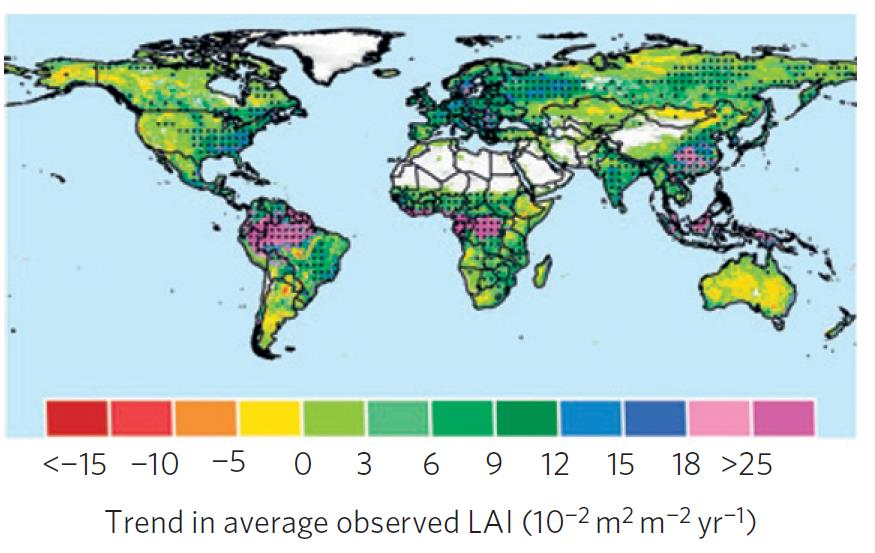
\includegraphics[width=1.0\textwidth]{bilder/bilderKlima-0002.jpg}\\[1cm]
\end{center}
\caption{Trends beim durchschnittlichen Blattflächenindex (LAI). Quelle: Zhu et al. 2016 Abbildung 3.}
\end{figure}

Piao et al. (2020) und Chen et al. (2024) berichten, dass der Ergrünungstrend ohne Anzeichen einer Verlangsamung fortsetzt, und CO$_2$-Düngung bleibt der dominante Treiber.

\subsection{Photosynthese und CO$_2$-Konzentrationen}

Pflanzen bauen Biomasse durch Photosynthese auf, einen Prozess, der Kohlendioxid, Wasser und Licht in Zucker umwandelt. Das für die Photosynthese verantwortliche Pflanzenenzym ist Ribulose-1,5-bisphosphat-carboxylase/oxygenase oder \emph{Rubisco}. Photosynthese wird eingeleitet, wenn CO$_2$ an der Oberfläche des Rubisco-Enzyms verfügbar ist, wo es in ein Molekül mit 3 Kohlenstoffatomen umgewandelt und danach in die Pflanzenmasse eingebaut wird. Dies wird als \emph{C3}-Prozess bezeichnet.

Rubisco wird geschätzt, vor etwa 3 Milliarden Jahren entstanden zu sein. Über geologische Zeit waren die atmosphärischen CO$_2$-Konzentrationen der Erde normalerweise viele Male höher als heute. Vor etwa 400 Millionen Jahren lagen CO$_2$-Konzentrationen schätzungsweise bei 2.000-4.000 ppm und waren für den größten Teil des Zeitraums von 200 bis 50 Millionen Jahren bei oder über 1.000 ppm (Berner 2006, Judd et al. 2024). Über die letzten 35 Millionen Jahre ist die atmosphärische CO$_2$-Konzentration stetig gefallen und fiel auf bis zu 170 ppm während Vereisung (Gerhart und Ward 2010). Während die moderne Änderungsrate von CO$_2$ im Vergleich zu früheren Zeiträumen hoch sein mag, zeigen die geologischen Beweise, dass Pflanzen und Tiere sich unter viel höheren CO$_2$-Konzentrationen als gegenwärtig entwickelten.

Als Antwort auf niedrige CO$_2$-Bedingungen entwickelten einige Pflanzen einen anderen photosynthetischen Weg namens \emph{C4}, bei dem CO$_2$ in der Nähe von Rubisco konzentriert wird, wodurch der \emph{C3}-Prozess effizienter funktionieren kann. Für landwirtschaftliche Zwecke sind die Pflanzenkategorien:
\begin{itemize}
\item C3: Reis, Weizen, Sojabohnen und die meisten anderen Feldfrüchte
\item C4: Mais, Zuckerrohr, Hirse, Sorghum	
\end{itemize}

Hätten atmosphärische CO$_2$-Konzentrationen weiter abgenommen, wäre das Pflanzenwachstum zurückgegangen und schließlich aufgehört. Unter \SI{180}{ppm} sind die Wachstumsraten vieler C3-Arten um 40-60 Prozent im Vergleich zu \SI{350}{ppm} reduziert (Gerhart und Ward 2010), und das Wachstum ist unter experimentellen Bedingungen von \SIrange{60}{140}{ppm} CO$_2$ vollständig zum Stillstand gekommen. Einige C4-Pflanzen können noch bei Konzentrationen von nur \SI{10}{ppm} wachsen, wenn auch sehr langsam (Gerhart und Ward 2010).


\begin{figure}[H]
\begin{center}
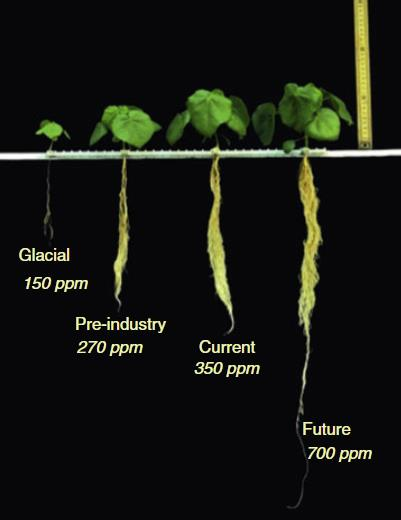
\includegraphics[width=0.7\textwidth]{bilder/bilderKlima-0003.jpg}\\[1cm]
\end{center}
\caption{Wachstum von \emph{Abutilon theophrasti} nach 14 Tagen unter identischen Bedingungen, jedoch mit den
angegebenen Schwankungen des CO2-Gehalts. Quelle: Gerhart und Ward (2010). Hinweis: „Aktuell” entspricht
1988 im Bild.}
\end{figure}

Die aktuellen CO$_2$-Konzentrationen liegen bei etwa \SI{430}{ppm}, gegenüber \SI{280}{ppm} in den frühen 1800er Jahren. Die positive Reaktion von Pflanzen auf zusätzliches CO$_2$ ist in Abbildung 2.2 dargestellt, reproduziert aus Gerhart und Ward (2010). Sie zeigt den Wachstumseffekt von CO$_2$ auf Samtpappel (Abutilon theophrasti) Sämlinge über 14 Tage unter kontrollierten Bedingungen, wo nur die CO$_2$-Exposition variiert wird. Die Zuwächse durch Erhöhung von CO$_2$ von \SI{150}{ppm} auf \SI{350}{ppm} setzen sich bei einer weiteren Verdopplung auf \SI{700}{ppm} fort.

Über die letzten 60+ Jahre gab es Tausende von Studien über die Reaktion von Pflanzen auf steigende CO$_2$-Konzentrationen. Das überwältigende Thema ist, dass Pflanzen, besonders C3-Pflanzen, von zusätzlichem CO$_2$ profitieren. Es gibt zwei Mechanismen, durch die CO$_2$ einen Wachstumsvorteil verleiht:

\begin{itemize}
\item Verstärkte Photosynthese über die oben beschriebenen Stoffwechselwege.
\item Erhöhte Wassernutzungseffizienz. Dies entsteht, weil Pflanzen CO$_2$ aufnehmen, indem sie die Stomata (Poren) auf der Blattoberfläche öffnen. Wenn CO$_2$ knapp ist, müssen die Stomata für lange Zeiträume weit offen gehalten werden, wodurch Wasser verdunsten kann. Unter angereicherten CO$_2$-Bedingungen bleiben die Stomata für längere Zeiträume geschlossen, wodurch die Pflanze Wasser länger zurückhalten kann und so die Wassernutzungseffizienz erhöht wird.
\end{itemize}

Spezifische Auswirkungen des Klimawandels auf die US-Landwirtschaft werden in Kapitel 9 überprüft.

\subsection{Steigendes CO$_2$ und Wassernutzungseffizienz von Feldfrüchten}

Deryng et al. (2016) untersuchten Beweise zur Wasserproduktivität von Feldfrüchten (CWP), dem Ertrag pro verwendete Wassereinheit, und lenkten Aufmerksamkeit auf das Potenzial von CO$_2$, sowohl die Photosynthese zu verstärken als auch die Transpiration auf Blattebene (Wasserverlust während der Blattatmung) zu reduzieren. Sie untersuchten alle verfügbaren FACE-Daten (Free Air CO$_2$ Enrichment—siehe Kapitel 9) zu Feldfruchtertragsänderungen für Mais, Weizen, Reis und Sojabohnen und kombinierten sie mit Feldfruchtemodell-Daten, die Ertragsreaktionen bis 2080 unter dem extremen RCP8.5-Emissionsszenario in vier Anbauregionen (Tropen, Trocken, Gemäßigt und Kalt) simulierten, von denen jede in regenabhängige und bewässerte Unterregionen aufgeteilt war. Sie berichteten, dass Modelle ohne CO$_2$-Düngung CWP-Verluste in jeder Region vorhersagten, aber diese wurden durch CO$_2$-Düngung mehr als ausgeglichen, sodass alle Regionen einen Netto-CWP-Gewinn zeigten.

Deryng et al. (2016) berichteten auch, dass negative Auswirkungen der Erwärmung auf Weizen- und Sojabohnenerträge vollständig durch CWP-Gewinne ausgeglichen und um bis zu 90 Prozent für Reis und 60 Prozent für Mais gemildert wurden.

Ähnlich bemerkten Cheng et al. (2017), dass die erhöhte Bruttoprimärproduktion von 1982 bis 2011 aufgrund steigender CO$_2$-Aufnahme von so großen CWP-Gewinnen begleitet war, dass der globale Wasserverbrauch von Pflanzen nicht gestiegen war, trotz der zusätzlichen Biomasse.

Deryng et al. (2016) nahmen an, dass Klimawandel \emph{Wasserknappheit verschärfen} würde. Doch während Modelle vorhersagen, dass Trockengebiete sich unter Klimaerwärmung ausdehnen werden, zeigen aktuelle Daten das Gegenteil: Ergrünung geschieht sogar in trockenen Gebieten. Zhang et al. (2024) berichten, dass aufgrund erhöhter CO$_2$-Konzentrationen \emph{zunehmende Trockenheit in Trockengebieten nicht zu einem allgemeinen Verlust der Vegetationsproduktivität führen wird}; höchstens 4 Prozent der derzeit trockenen Gebiete werden erhöhte Wüstenbildung erleben.

\subsection{CO$_2$-Düngungsvorteile in IPCC-Berichten}

Das IPCC hat globale Ergrünung und CO$_2$-Düngung landwirtschaftlicher Feldfrüchte nur minimal diskutiert. Das Thema wird kurz an einigen Stellen im Hauptteil des 6. und früherer IPCC-Bewertungsberichte anerkannt, aber in allen Zusammenfassungsdokumenten weggelassen. Abschnitt 2.3.4.3.3 des AR6 Working Group I-Berichts, betitelt \emph{globale Ergrünung und Bräunung}, weist darauf hin, dass der IPCC-Sonderbericht über Klimawandel und Land mit hoher Zuversicht geschlossen hatte, dass Ergrünung global über die letzten 2-3 Jahrzehnte zugenommen hatte. Er diskutiert dann, dass es Variationen im Ergrünungstrend zwischen Datensätzen gibt, und schließt, dass sie zwar hohe Zuversicht haben, dass Ergrünung aufgetreten ist, aber niedrige Zuversicht in das Ausmaß des Trends. Es gibt auch kurze Erwähnungen von CO$_2$-Düngungseffekten und Verbesserungen der Wassernutzungseffizienz in einigen anderen Kapiteln der AR6 Working Groups I und II-Berichte.

Insgesamt diskutieren jedoch die Policymaker Summaries, Technical Summaries und Synthesis Reports von AR5 und AR6 das Thema nicht.


\section{Die alkalischen Ozeane}

\subsection{Verändernder pH-Wert}

Eine neutrale wässrige Lösung hat einen pH-Wert von 7,0, während eine mit pH größer als 7,0 alkalisch (auch basisch genannt) und mit pH kleiner als 7,0 sauer ist. Der heutige globale Durchschnitts-pH-Wert von Oberflächenmeerwasser wird auf 8,04 geschätzt (\emph{Copernicus Marine Service 2025}, Abbildung 2.3), gegenüber einem geschätzten Wert von 8,2 in vorindustrieller Zeit (Gattuso und Hansson, 2011). Als CO$_2$-Konzentrationen in der Atmosphäre stiegen, absorbierten die Ozeane mehr, was ihren pH-Wert senkt. Abhängig von der Pufferkapazität der Ozeane wird erwartet, dass sie mit der Zeit etwas weniger alkalisch werden, was mit dem beobachteten pH-Rückgang übereinstimmt.

\begin{figure}[H]
\begin{center}
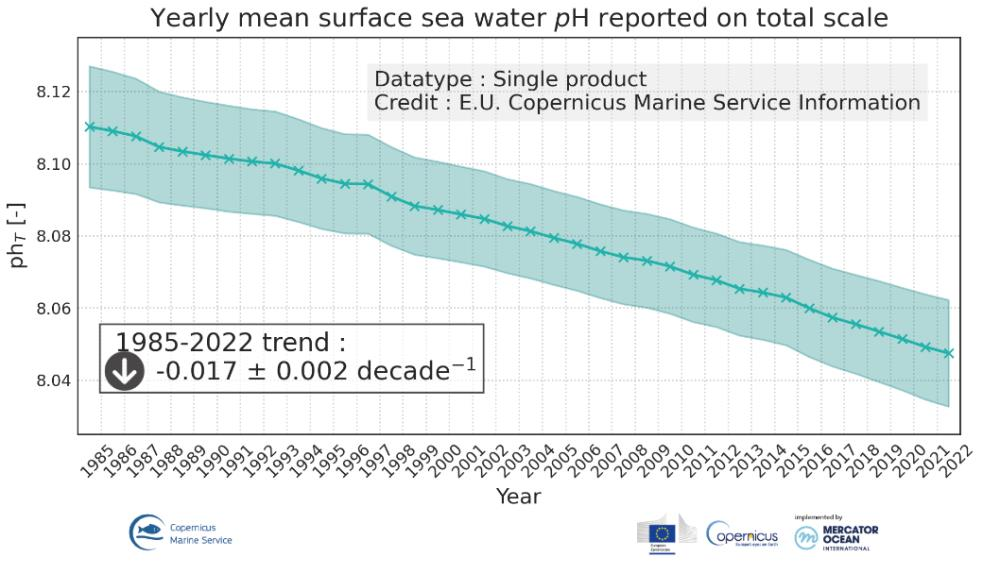
\includegraphics[width=1.0\textwidth]{bilder/bilderKlima-0004.jpg}\\[1cm]
\end{center}
\caption{pH-Wert der Ozeane 1985–2022. Quelle: Copernicus Marine Service 2025}
\end{figure}

Während dieser Prozess oft \emph{Ozeanversauerung} genannt wird, ist das eine Fehlbezeichnung, weil nicht erwartet wird, dass die Ozeane sauer werden; \emph{Ozeanneutralisierung} wäre genauer. Selbst wenn das Wasser sauer würde, wird angenommen, dass sich Leben in den Ozeanen entwickelte, als die Ozeane leicht sauer mit pH 6,5 bis 7,0 waren (Krissansen-Totton et al., 2018). Auf der Zeitskala von Tausenden von Jahren zeigen Bor-Isotop-Proxy-Messungen, dass der Ozean-pH-Wert während der letzten Vereisung (bis vor etwa 20.000 Jahren) um 7,4 oder 7,5 lag und auf heutige Werte anstieg, als sich die Welt während der Enteisung erwärmte (Rae et al., 2018). Somit scheinen Ozeanbiota widerstandsfähig gegenüber natürlichen langfristigen Veränderungen des Ozean-pH-Werts zu sein, da Meeresorganismen einer weiten Bandbreite von pH-Werten ausgesetzt waren.

\subsection{Korallenriff-Veränderungen}

Es gibt Bedenken, dass ein abnehmender pH-Wert des Meerwassers die Verkalkungsrate von Korallenriffen reduzieren wird. Aber Korallenriffe ertragen bereits große pH-Schwankungen, teilweise aufgrund täglicher photosynthetischer Aktivität im Riff; gemessene pH-Werte reichen von 9,4 während des Tages bis 7,5 nachts (Revelle und Fairbridge, 1957). De'ath et al. (2009) berichteten, dass Verkalkungsraten am Great Barrier Reef von 1990 bis 2005 um 14,2 Prozent zurückgegangen waren. Ridd et al. (2013) verwendeten jedoch andere Methoden und fanden keinen signifikanten Trend in den Verkalkungsraten.

Jüngste Daten vom Australian Institute of Marine Science zeigen, dass sich das Great Barrier Reef stark erholt hat. Der Korallenbedeckungsgrad erreichte 2022 36-Jahres-Höchststände in zwei Dritteln des Riffs. Das Institute kommentierte: \emph{Das war das dritte Jahr in Folge mit weit verbreiteter Erholung} (Australian Institute of Marine Science, 2022). Die \emph{Woods Hole Oceanographic Institution} bemerkte 2023: \emph{Das Great Barrier Reef macht ein bemerkenswertes Comeback} (Woods Hole Oceanographic Institution, 2023).

\begin{figure}[H]
\begin{center}
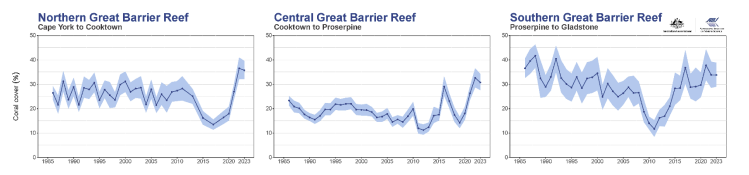
\includegraphics[width=1.0\textwidth]{bilder/bilderKlima-0005.png}\\[1cm]
\end{center}
\caption{Hartkorallenbedeckung in drei Regionen des \emph{Great Barrier Reef} von 1985 bis 2023. Quelle: AIMS 2023.}
\end{figure}

Es scheint, dass Korallen anpassungsfähiger sind als früher gedacht. Die Vorfahren moderner Korallen erschienen vor etwa 245 Millionen Jahren. CO$_2$-Konzentrationen waren für mehr als 200 Millionen Jahre danach viele Male höher als heute. Ein Großteil der öffentlichen Diskussion über die Auswirkungen der Ozean-"Versauerung" auf Meeresbiota war einseitig und übertrieben.

Ähnlich fand eine Meta-Analyse (Clements et al., 2021) der negativen Auswirkungen der Ozeanversauerung auf das Verhalten von Rifffischen das, was sie einen \emph{Decline-Effekt} nannten: anfänglich dramatische Schlussfolgerungen, die in prominenten Zeitschriften veröffentlicht wurden und scheinbar große Auswirkungen der Versauerung zeigten, tendierten dazu, von nachfolgenden Studien mit größeren Stichprobengrößen gefolgt zu werden, die viel kleinere und typischerweise nicht-existente Effekte ergaben. Sie fordern ihre Kollegen auf, Forschungspraktiken zu verbessern, um dem \emph{Decline-Effekt} entgegenzuwirken:

Die überwiegende Mehrheit der Studien mit großen Effektgrößen in diesem Bereich tendiert dazu, durch niedrige Stichprobengrößen charakterisiert zu sein, wird aber dennoch in hochrangigen Zeitschriften veröffentlicht und hat einen unverhältnismäßigen Einfluss auf das Feld in Bezug auf Zitationen. Wir behaupten, dass Ozeanversauerung einen vernachlässigbaren direkten Einfluss auf Fischverhalten hat, und wir setzen uns für verbesserte Ansätze ein, um das Potenzial für einen Decline-Effekt in zukünftigen Forschungsrichtungen zu minimieren (Clements et al., 2021).

Zusammenfassend ist Meeresleben komplex, und vieles davon entwickelte sich, als die Ozeane relativ zur Gegenwart sauer waren. Die Vorfahren moderner Korallen erschienen vor etwa 245 Millionen Jahren. CO$_2$-Konzentrationen waren für mehr als 200 Millionen Jahre danach viele Male höher als heute. Ein Großteil der öffentlichen Diskussion über die Auswirkungen der Ozean-"Versauerung" auf Meeresbiota war einseitig und übertrieben.

\vfill
\noindent\textbf{Literaturverzeichnis:}

\begingroup
\parindent=0pt
\everypar{\hangindent=2em\hangafter=1\relax}

AR6: Intergovernmental Panel on Climate Change Sixth Assessment Report (2021) Working Group I Contribution. www.ipcc.ch.

Australian Institute of Marine Science. (2022). Continued coral recovery leads to 36-year highs across two-thirds of the Great Barrier Reef. \url{https://www.aims.gov.au/sites/default/files/2022-08/AIMS_LTMP_Report_on\%20GBR_coral_status_2021_2022_040822F3.pdf}

Beeden, R., Maynard, J., Puotinen, M., Marshall, P., Dryden, J., Goldberg, J., and Williams, G. (2015). Impacts and recovery from Severe Tropical Cyclone Yasi on the Great Barrier Reef. PLOS ONE, 10, e0121272. https://doi.org/10.1371/journal.pone.0121272

Berner, R. A. (2006). GEOCARBSULF: A combined model for Phanerozoic atmospheric O$_2$ and CO$_2$. Geochimica et Cosmochimica Acta, 70, 5653–5664.

Browman, H. I. (2016). Applying organized scepticism to ocean acidification research. ICES Journal of Marine Science, 73(3), 529.1–536. https://doi.org/10.1093/icesjms/fsw010

Chen, C., Park, T., Wang, X., Piao, S., Xu, B., Chaturvedi, R. K., and Myneni, R. B. (2019). China and India lead in greening of the world through land-use management. Nature Sustainability, 2, 122–129. https://www.nature.com/articles/s41893-019-0220-7

Chen, X., Wang, Y., Liu, Y., and Piao, S. (2024). The global greening continues despite increased drought stress since 2000. Global Ecology and Conservation, 49, e02791. https://www.sciencedirect.com/science/article/pii/S2351989423004262

Cheng, L., Zhang, L., Wang, Y. P., et al. (2017). Recent increases in terrestrial carbon uptake at little cost to the water cycle. Nature Communications, 8, 110. https://doi.org/10.1038/s41467-017-00114-5

Clements, J. C., Sundin, J., Clark, T. D., and Jutfelt, F. (2022). Meta-analysis reveals an extreme "decline effect" in the impacts of ocean acidification on fish behavior. PLOS Biology, 20(2), e3001511. https://doi.org/10.1371/journal.pbio.3001511

Copernicus Marine Service. (2025). Global ocean acidification – Mean sea water pH time series and trend from multi-observations reprocessing. \url{https://data.marine.copernicus.eu/product/GLOBAL_OMI_HEALTH_carbon_ph_area_averaged/description}

De'ath, G., Lough, J., and Fabricius, K. (2009). Declining coral calcification on the Great Barrier Reef. Science, 323, 116–119. https://doi.org/10.1126/science.1165283

Deryng, D., Conway, D., Ramankutty, N., Price, J., Warren, R., Jones, R., ... and Elliott, J. (2016). Regional disparities in the beneficial effects of rising CO$_2$ concentrations on crop water productivity. Nature Climate Change. https://doi.org/10.1038/nclimate2995

Gattuso, J. P., and Hansson, L. (Eds.). (2011). Ocean acidification: Background and history. Oxford University Press.

Gerhart, L. M., and Ward, J. K. (2010). Plant responses to low [CO$_2$] of the past. New Phytologist, 188, 674–695. https://nph.onlinelibrary.wiley.com/doi/pdf/10.1111/j.1469-8137.2010.03441.x

Haverd, V., B. Smith, J. G. Canadell, et al. (2020). Higher than expected CO$_2$ fertilization inferred from leaf to global observations. Global Change Biology, 26, 2390–2402. https://doi.org/10.1111/gcb.14950

Keenan, T. F., X. Luo, B. D. Stocker, et al. (2023). A constraint on historic growth in global photosynthesis due to rising CO2. Nature Climate Change 13(12): 1376-1381 DOI: 10.1038/s41558-023-01867-2.

Judd, E. J., Scotese, C. R., Young, S. A., et al. (2024). A 485-million-year history of Earth's surface temperature. Science, 385(6715). https://doi.org/10.1126/science.adk3705

Krissansen-Totton, J., Arney, G. N., and Catling, D. C. (2018). Constraining the climate and ocean pH of the early Earth with a geological carbon cycle model. Proceedings of the National Academy of Sciences, 115(6), 4105–4110. https://doi.org/10.1073/pnas.1721296115

Piao, S., X. Wang, T. Park, et al. (2020). Characteristics, drivers and feedbacks of global greening. Nature Reviews Earth \& Environment 1(1): 14-27 DOI: 10.1038/s43017-019-0001-x

Rae, J. W. B., Burke, A., Robinson, L. F., et al. (2018). CO$_2$ storage and release in the deep Southern Ocean on millennial to centennial timescales. Nature, 562, 569–573. https://doi.org/10.1038/s41586-018-0614-0

Revelle, R., and Fairbridge, R. W. (1957). Carbonate and carbon dioxide. In J. W. Hedgpeth (Ed.), Treatise on marine ecology and paleoecology (Vol. 1). Geological Society of America.

Ridd, P., Silva, E., and Stieglitz, T. (2013). Have coral calcification rates slowed in the last twenty years? Marine Geology, 346, 392–399. https://doi.org/10.1016/j.margeo.2013.09.002

Woods Hole Oceanographic Institution. (2023). Is the Great Barrier Reef making a comeback? https://www.whoi.edu/oceanus/feature/is-the-great-barrier-reef-making-a-comeback/

Zeng, Z., Piao, S. Li, L., et al. (2017). Climate mitigation from vegetation biophysical feedbacks during the past three decades. Nature Climate Change. https://doi.org/10.1038/nclimate3299

Zhang, Y., Liu, Y., Chen, X., et al. (2024). Less than 4% of dryland areas are projected to desertify despite increased aridity under climate change. Nature Communications Earth and Environment, 5. https://www.nature.com/articles/s43247-024-01463-y

Zhu, Z., Piao, S., Myneni, R. B., et al. (2016). Greening of the Earth and its drivers. Nature Climate Change, 6, 791–795. https://www.nature.com/articles/nclimate3004
\endgroup

%\numberwithin{figure}{section}
\FigureNumbersBySection
\chapter{Menschliche Einflüsse auf das Klima}
\paragraph{Kapitelzusammenfassung}
\begin{quote}
Das globale Klima ist natürlicherweise auf allen Zeitskalen variabel. Anthropogene CO$_2$-Emissionen verstärken diese Variabilität, indem sie die gesamte Strahlungsenergiebilanz in der Atmosphäre verändern.

Das IPCC hat die Rolle der Sonne beim Klimawandel herabgespielt, aber es gibt plausible Rekonstruktionen der Sonneneinstrahlung, die darauf hindeuten, dass sie zur jüngsten Erwärmung beigetragen hat.

Klimaprojektionen basieren auf IPCC-Emissionsszenarien, die dazu tendierten, beobachtete Trends zu übertreffen. Die meisten akademischen Klimaauswirkungsstudien der letzten Jahre basieren auf dem extremen RCP 8.5-Szenario, das jetzt als unplausibel gilt; seine Verwendung als Business-as-usual-Szenario war irreführend.

Kohlenstoffkreislaufmodelle verbinden jährliche Emissionen mit dem Wachstum des atmosphärischen CO$_2$-Bestands. Während sich Modelle über die Rate der Land- und Ozean-CO$_2$-Aufnahme uneinig sind, stimmen alle darin überein, dass sie seit 1959 gestiegen ist.

Es gibt Belege dafür, dass Urbanisierungsverzerrungen in der Landerwärmungsaufzeichnung nicht vollständig aus Klimadatensätzen entfernt wurden.
\end{quote}

\section{Komponenten der Strahlungsantriebe und ihre Geschichte}
\subsection{Historischer Strahlungsantrieb}
Ein sich veränderndes Klima war die Norm während der gesamten 4.6 Milliarden Jahre langen Geschichte der Erde. Die Temperatur und Wettermuster der Erde verändern sich natürlich über Zeitskalen von Jahrzehnten bis zu Millionen von Jahren. Natürliche Variationen des Oberflächenklimas entstehen auf zwei Wegen. Interne Klimaschwankungen im Zusammenhang mit Zirkulationen in der Atmosphäre und den Ozeanen tauschen Energie, Wasser und Kohlenstoff zwischen der Atmosphäre, Ozeanen, Land und Eis aus. Externe Einflüsse auf das Klimasystem umfassen Variationen in der von der Sonne empfangenen Energie und die Auswirkungen von Vulkanausbrüchen. Menschliche Aktivitäten beeinflussen das Klima durch Veränderungen der Landnutzung und Landbedeckung. Menschen verändern auch die Zusammensetzung der Atmosphäre durch Emissionen von CO$_2$ und anderen Treibhausgasen und durch die Veränderung der Konzentration von Aerosolpartikeln in der Atmosphäre.

Die Erde wird durch das Sonnenlicht erwärmt, das sie absorbiert, und wird durch die Wärme gekühlt, die sie in den Weltraum abstrahlt. Über die Erdoberfläche gemittelt, beinhalten diese Prozesse jeweils Energieflüsse von etwa 240 Watt pro Quadratmeter (W/m²). Wenn sie im Gleichgewicht sind, gibt es keine äußeren Ursachen für Erwärmung oder Abkühlung. Sowohl menschliche als auch natürliche Einflüsse auf das Klima verändern dieses Gleichgewicht und verursachen damit Klimaveränderungen.

Einflüsse auf die Energiebilanz der Erde an der Spitze der Atmosphäre werden durch \emph{Strahlungsantrieb} quantifiziert, das Ausmaß, in dem sie das Erwärmungs-/Abkühlungsgleichgewicht stören; ein positiver Antrieb erwärmt, während ein negativer Antrieb kühlt. Die geschätzte Geschichte der wichtigsten Komponenten des Strahlungsantriebs seit 1750 durch das IPCC ist in den folgenden zwei Abbildungen aus seinem AR6 dargestellt.

\begin{figure}[H]
\begin{center}
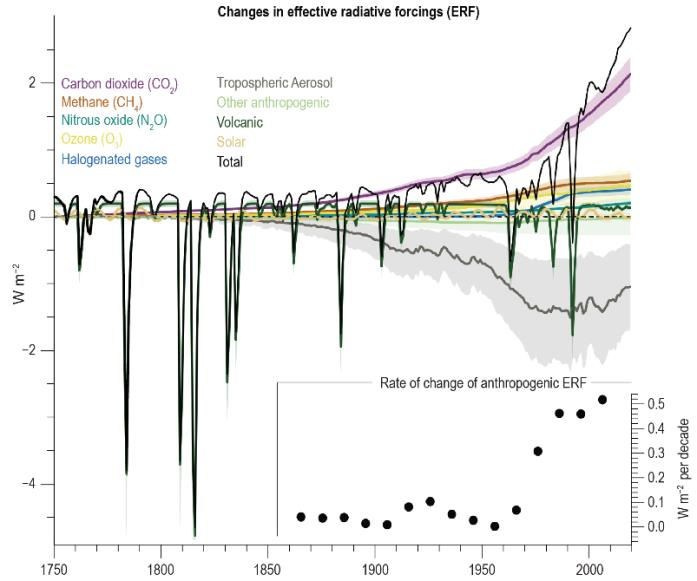
\includegraphics[width=1.0\textwidth]{bilder/bilderKlima-0006.jpg}\\[1cm]
\end{center}
\caption{IPCC-Schätzungen der Komponenten des Strahlungsantriebs im Zeitverlauf. Die Schattierung zeigt
die Unsicherheitsbereiche an. Quelle: AR6 WGI Ch2 Abb. 10}
\end{figure}

\begin{figure}[H]
\begin{center}
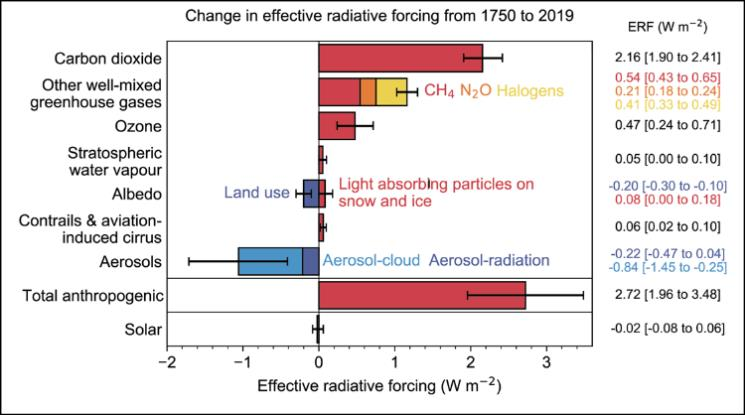
\includegraphics[width=1.0\textwidth]{bilder/bilderKlima-0007.jpg}\\[1cm]
\end{center}
\caption{IPCC-Schätzungen der Veränderungen der Strahlungsantriebskomponenten von 1750 bis 2019. Quelle:
AR6 WGI Kap. 7 Abb. 7-6.}
\end{figure}

Diese Grafiken zeigen, dass der gesamte Strahlungsantrieb sowohl aus natürlichen als auch aus anthropogenen Komponenten besteht. Kohlendioxid ist der größte menschliche Einfluss auf das Klima und derjenige, der am relevantesten für den Einfluss der Nutzung fossiler Brennstoffe ist. Es übt einen erwärmenden Einfluss aus, indem es die Kühlkraft der Atmosphäre verringert. CO$_2$-Emissionen akkumulieren in der Atmosphäre, wie im folgenden Abschnitt beschrieben, sodass der erwärmende Einfluss wächst.

Andere anthropogene Strahlungsantriebe umfassen andere Treibhausgase (Methan, Lachgas, fluorierte Gase), Aerosole und Landnutzungsänderungen. Es gibt jedoch erhebliche Unsicherheiten in diesen Komponenten. Das IPCC identifiziert Wolken-Aerosol-Wechselwirkungen als die größte Unsicherheit im gesamten Strahlungsantrieb.

Eine wichtige natürliche Komponente ist die Sonneneinstrahlung. Variationen in der Sonnenaktivität sind gut dokumentiert und können das Klima beeinflussen. Das IPCC hat jedoch die Rolle solarer Variabilität beim Klimawandel heruntergespielt. Soon et al. (2021) stellten fest, dass die Konsensaussagen des IPCC zum solaren Antrieb vorzeitig durch die Unterdrückung abweichender wissenschaftlicher Meinungen formuliert wurden.

Eine weitere natürliche Strahlungsantriebskomponente sind vulkanische Aerosole, die einen episodischen kühlenden Einfluss ausüben. Box 4.1 im IPCC AR6-Bericht behandelt die Klimaauswirkungen von Vulkanausbrüchen und bemerkt drei explosive Vulkanausbrüche, die in der ersten Hälfte des 19. Jahrhunderts auftraten. Dazu gehörte der Tambora-Ausbruch von 1815, der zum 'Jahr ohne Sommer' führte, mit mehreren Ernteausfällen in der gesamten Nordhalbkugel. Es gibt Unsicherheit über das Vorzeichen der relativ kleinen Antriebskraft des Unterwasservulkans Hunga Tonga, der 2022 ausbrach (Jenkins et al. 2023, Schoeberl et al. 2024).

Abbildung 3.1.1 zeigt, dass die anthropogene Antriebskomponente vor etwa 1900 vernachlässigbar war und seitdem stetig gestiegen ist und heute auf fast \SI{3}{\watt\per\square\meter} angestiegen ist. Dies ist jedoch immer noch nur etwa 1 Prozent der ungestörten Strahlungsflüsse, was es zu einer Herausforderung macht, die Auswirkungen des anthropogenen Antriebs zu isolieren; modernste Satellitenschätzungen globaler Strahlungsenergieflusse sind nur auf wenige \si{\watt\per\square\meter} genau.

Natürliche Quellen globaler Energieungleichgewichte außer Vulkanen und der gesamten Sonneneinstrahlung (TSI) sind in diesen Grafiken nicht enthalten, da sie weitgehend unbekannt bleiben.

\subsection{Veränderung des atmosphärischen CO$_2$ seit 1958}

Der erwärmende Einfluss von Kohlendioxid hängt davon ab, wie viel \emph{zusätzliches} CO$_2$ sich in der Atmosphäre ansammelt – d.h. seine Konzentration über dem vorindustriellen Wert von \SI{280}{ppm}. Der CO$_2$-Gehalt, wie er am Mauna Loa-Observatorium in Hawaii aufgezeichnet wird, der allgemein als repräsentative globale Durchschnittskonzentration verwendet wird, ist online verfügbar unter \url{https://gml.noaa.gov/ccgg/trends/index.html}. Die Konzentration lag zu Beginn der Aufzeichnung 1959 bei etwa \SI{316}{ppm} und liegt jetzt bei etwa \SI{430}{ppm}, ein Anstieg von 36 Prozent. Am Ende der letzten Vereisung waren die CO$_2$-Konzentrationen auf etwa \SI{180}{ppm} gefallen. Wie in Kapitel 2 diskutiert, beginnen C3-Pflanzen bei CO$_2$-Konzentrationen unter etwa \SI{140}{ppm} zu sterben und C4-Pflanzen bei Konzentrationen unter \SI{100}{ppm}, sodass bei weiterem Fallen der CO$_2$-Konzentrationen das Pflanzenleben gefährdet gewesen wäre.


\begin{figure}[H]
\begin{center}
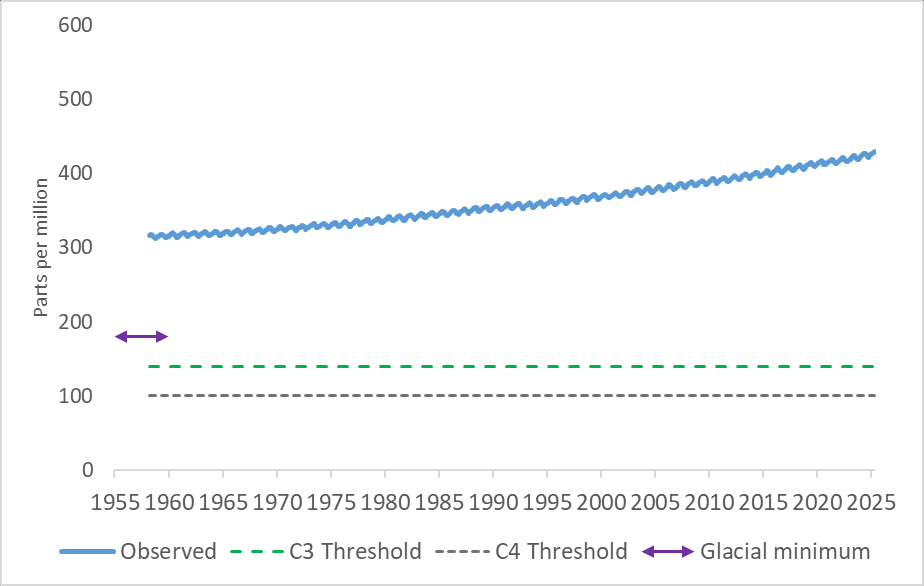
\includegraphics[width=1.0\textwidth]{bilder/bilderKlima-0009.png}\\[1cm]
\end{center}
\caption{Jährliche durchschnittliche CO2-Konzentrationen in der Atmosphäre (1959–2025) in ppm, gemessen am
Mauna Loa (blau). C3-Schwellenwert: Wert, unterhalb dessen C3-Pflanzen zu sterben beginnen (140 ppm, siehe
Kapitel 2). C4-Schwellenwert: Wert, unterhalb dessen C4-Pflanzen zu sterben beginnen (100 ppm, siehe Kapitel 2).
Glaziales Minimum: Mindestniveau während der letzten Eiszeiten (lila Pfeil). CO2-Datenquelle:
\url{https://gml.noaa.gov/ccgg/trends/index.html}}
\end{figure}

Der jährliche Konzentrationsanstieg ist nur etwa die Hälfte des emittierten CO$_2$, weil Land- und Ozeanprozesse derzeit \emph{überschüssiges} CO$_2$ mit einer Rate von etwa 50 Prozent der menschlichen Emissionen absorbieren. Zukünftige Konzentrationen und damit zukünftige menschliche Einflüsse auf das Klima hängen daher von zwei Komponenten ab: (1) zukünftige Raten globaler menschlicher CO$_2$-Emissionen und (2) wie schnell Land und Ozean zusätzliches CO$_2$ aus der Atmosphäre entfernen. Wir diskutieren jede dieser der Reihe nach.

\section{Zukünftige Emissionsszenarien und der Kohlenstoffkreislauf}

\subsection{Emissionsszenarien}

Die Bewertung der Gefahren zukünftiger THG-Emissionen erfordert Annahmen darüber, was diese Emissionen sein werden. Zukünftige Emissionen und damit menschliche Einflüsse auf das Klima werden von zukünftiger Demografie, Wirtschaftstätigkeit, Regulierung sowie Energie- und Agrartechnologien abhängen. Verschiedene Annahmen über jeden dieser Faktoren führen zu Projektionen von Treibhausgasemissionen und -konzentrationen, Aerosolkonzentrationen und Veränderungen der Landnutzung, die letztendlich zu Annahmen über anthropogenen Strahlungsantrieb kombiniert werden können.

Die großen Unsicherheiten über diese vielen Faktoren machen es unmöglich, zukünftige Emissionen präzise vorherzusagen. Stattdessen hat das IPCC verschiedene Szenario-Sets verwendet, die einen plausiblen Bereich von Möglichkeiten für Bevölkerung, Wirtschaft und Technologien abdecken sollen. Jüngste Versionen der Szenarien sind durch eine Zahl gekennzeichnet, die den anthropogenen Strahlungsantrieb angibt, der 2100 unter diesem Szenario erwartet wird. So entspricht ein mit "6" bezeichnetes Szenario \SI{6}{\watt\per\square\meter} menschlich induziertem Strahlungsantrieb (Erwärmung) am Ende des Jahrhunderts. (Erinnern Sie sich, der aktuelle anthropogene Strahlungsantrieb beträgt etwa \SI{2.7}{\watt\per\square\meter}.)

Obwohl das IPCC nicht behauptet, dass seine Emissionsszenarien Vorhersagen sind, werden sie oft als solche behandelt. Vergleiche vergangener Szenario-Gruppen mit Beobachtungen zeigen, dass IPCC-Emissionsprojektionen dazu tendierten, tatsächliche nachfolgende Emissionen zu überschätzen. Für den dritten und vierten IPCC-Bewertungsbericht wurde eine Reihe von Emissionsprojektionen aus dem Sonderbericht zu Emissionsszenarien verwendet; diese wurden als SRES-Szenarien bezeichnet. McKitrick et al. (2012) zeigten, dass die SRES-Szenario-Emissionsverteilung bei Umrechnung in Pro-Kopf-Werte im Vergleich zu beobachteten Trends nach oben verzerrt war. Die Verzerrung der SRES-Szenarien wurde durch die spätere Analyse von Hausfather et al. (2019) bestätigt, die zeigten, dass beobachtete atmosphärische CO$_2$-Konzentrationen dem unteren Ende des SRES-Bereichs und auch nachfolgender IPCC-Szenario-Bereiche folgten (Abbildung 3.2.1).

Für AR5 entwickelte das IPCC ein neues Set von Szenarien, die \emph{Representative Concentration Pathways} (RCPs) genannt wurden. Diese wurden durch eine Zahl identifiziert, die den Anstieg im Antrieb repräsentierte, und wurden daher RCP2.6, RCP4.5, RCP6.0 und RCP8.5 genannt. RCP2.6 (was einen anthropogenen Strahlungsantrieb 2100 von \SI{2.6}{\watt\per\square\meter} impliziert) beschreibt einen THG-Konzentrationspfad, der zu einer Erwärmung deutlich unter 2°C führt. Am anderen Ende der Skala ist RCP8.5 ein extremes Ergebnis, das fast \SI{5}{\celsius} Erwärmung von 1900 bis 2100 impliziert.

RCP8.5 kam dazu, als \emph{No-Policy-Baseline} oder \emph{Business-as-usual}-Szenario sowohl in der akademischen Literatur als auch in den populären Medien bezeichnet zu werden. Es wurde daher verwendet, um das Referenzergebnis zu generieren, das angeblich die Welt des 21. Jahrhunderts in Abwesenheit zunehmend strenger Emissionsreduktionspolitiken repräsentiert. Aber RCP8.5 war als ein Niedrig-Wahrscheinlichkeits-Hochemmissionsszenario gedacht, und seine Verwendung als Business-as-usual-Baseline wurde als grob irreführend kritisiert.\footnote{Dieses extreme Szenario ist nützlich für Modellierer, da ein großer Antrieb eine große Antwort (Erwärmung) generiert, was es einfacher macht, die Sensitivität eines Modells zu bewerten. Aber das ist sehr unterschiedlich davon, zu behaupten, es sei ein plausibles zukünftiges Ergebnis.} Hausfather und Peters (2020a), die in einem Kommentar in Nature schrieben, wiesen darauf hin, dass RCP8.5 als ein extremer Worst-Case entwickelt wurde, und sein Missbrauch als \emph{Business as usual}-Baseline hat zu einer großen Anzahl irreführender Studien und Medienberichterstattung geführt.

Die Unplausibilität des RCP8.5-Szenarios wurde von Burgess et al. (2021) untersucht. Die Unplausibilität von RCP8.5 sollte nicht als sehr unwahrscheinlich (z.B. 95. Perzentil) oder ein \emph{Worst Case} interpretiert werden, sondern eher als genuinen unplausibel aufgrund der Unplausibilität der Inputs, die erforderlich sind, um einen Antrieb von \SI{8.5}{\watt\per\square\meter} zu erreichen. Sie bemerkten, dass RCP8.5 bereits von beobachteten Trends in der Energienutzung abgewichen ist und die nahen zukünftigen Trends scharf von denen der Internationalen Energieagentur (IEA) abweichen, die marktbasierte Projektionen der Energienutzung für die kommenden Jahrzehnte bereitstellt. Pielke Jr. et al. (2022) zeigten weiter, dass die historischen und projizierten IEA-Trends nahe dem Boden der Umhüllungen sowohl der RCP-Projektionen als auch der jüngeren Shared Socioeconomic Pathway (SSP)-Szenario-Trends verlaufen.

Schwalm et al. (2020) verteidigten die Verwendung von RCP8.5 mit der Begründung, dass kumulative CO$_2$-Emissionen über 2005-2020 es enger verfolgen als die niedrigeren RCP-Szenarien. Sie argumentieren auch, dass eine modifizierte Version der IEA-Szenarien RCP8.5 in den kommenden Jahrzehnten eng verfolgt. Hausfather und Peters (2020b) antworteten, dass die Fertigkeit von RCP8.5 über diese 15 Jahre auf ausgleichende Fehler in seiner Repräsentation von CO$_2$ aus Brennstoffnutzung und Landnutzungsänderung zurückzuführen ist, und die scheinbare Übereinstimmung mit IEA in kommenden Jahrzehnten ist darauf zurückzuführen, dass Schwalm et al. sehr hohe Landnutzungsemissionen hinzufügten. Die eigenen projizierten CO$_2$-Emissionen der IEA verfolgen deutlich unter RCP8.5.

Weitverbreitete Verwendung von RCP8.5 als No-Policy-Baseline hat eine Verzerrung in Richtung Alarm in der Klimaauswirkungsliteratur geschaffen. Das Ausmaß dieses Problems wurde in einer Literaturanalyse von Pielke Jr. und Ritchie (2020) bestätigt. Sie fanden, dass etwa 16.800 wissenschaftliche Arbeiten, die zwischen 2010 und 2020 veröffentlicht wurden, das RCP8.5-Szenario verwendeten, wobei etwa 4.500 der Artikel RCP8.5 mit dem Konzept von \emph{Business-as-usual} verknüpften. Ihre Analyse zeigte, wie RCP8.5 nicht nur von einzelnen Forschern missbraucht wurde, sondern auch von einflussreichen Wissenschaftsagenturen wie dem IPCC und dem U.S. National Climate Assessment (USNCA), was direkt zu irreführender Berichterstattung in prominenten Medien geführt hat.

\begin{figure}[H]
\begin{center}
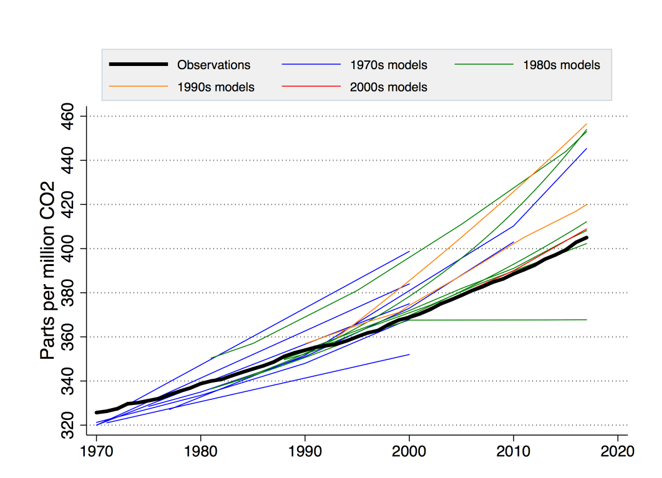
\includegraphics[width=1.0\textwidth]{bilder/bilderKlima-0011.png}\\[1cm]
\end{center}
\caption{Seit den 1970er Jahren haben aufeinanderfolgende Familien von Emissions- und Konzentrationsprognosen (farbige
Linien) die Beobachtungen (schwarze Linie) durchweg überschätzt. Quelle: Hausfather et al. (2019)
Abbildung S4.}
\end{figure}

Pielke und Ritchie (2020) berichteten, dass neue Studien, die RCP8.5 verwendeten, mit einer Rate von etwa 20 pro Tag veröffentlicht wurden, wobei etwa zwei pro Tag spezifisch RCP8.5 und \emph{business as usual} verknüpften. Sie schließen, dass die Klimaforschungsgemeinschaft ein Jahrzehnt damit verbracht hat, \emph{wissenschaftliche Ressourcen für Science Fiction zu verwenden} und dass \emph{Die wissenschaftliche Literatur ist in eine apokalyptische Richtung unausgewogen geworden.}

Das IPCC entwickelte ein neues Set von Szenarien für AR6, die \emph{Shared Socioeconomic Pathway} (SSP)-Szenarien, die die in den RCP- und SRES-Szenarien gezeigte Verzerrung fortgesetzt haben. Abbildung 3.2.2 zeigt die von der Internationalen Energieagentur (IEA) zusammengestellten gesamten globalen beobachteten CO$_2$-Emissionen, zusammengeführt mit der Emissionsprojektion der EIA unter Berücksichtigung von Energienutzungsprojektionen und aktuellen Politiken. Die anderen Linien zeigen den Bereich der IPCC SSP-Szenarien (SSP1-SSP5). Ab 2023 lagen globale CO$_2$-Emissionen deutlich unter SSP7.0 und waren sogar unter SSP2-4.5.

\begin{figure}[H]
\begin{center}
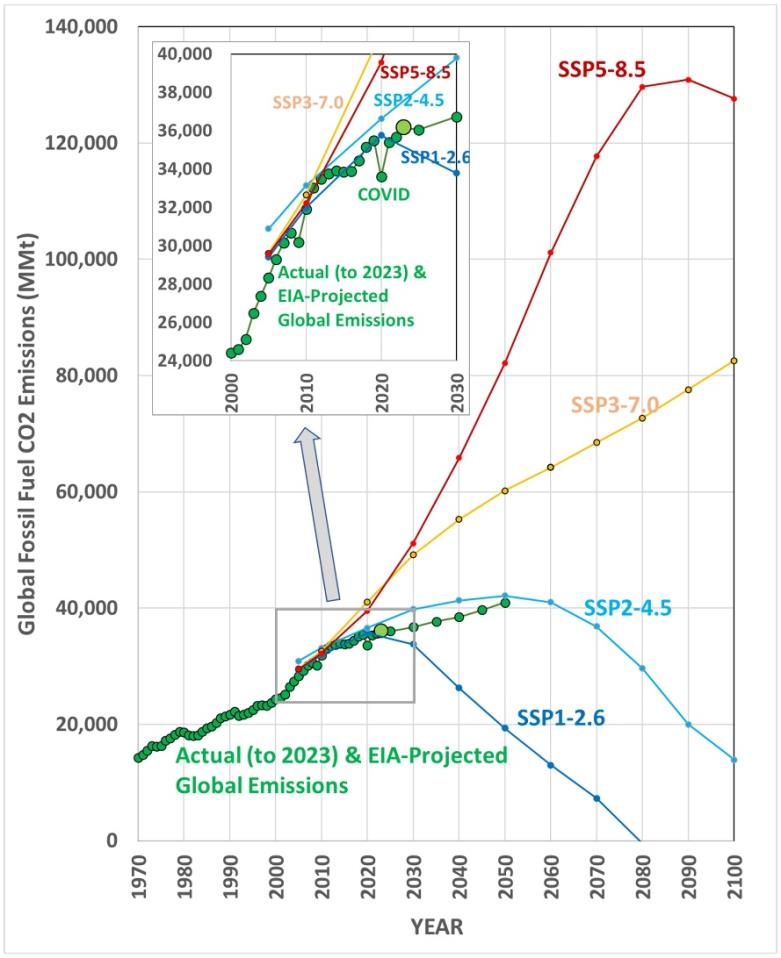
\includegraphics[width=1.0\textwidth]{bilder/bilderKlima-0012.jpg}\\[1cm]
\end{center}
\caption{Beobachtete und prognostizierte CO$_2$-Emissionen. Quelle: IPCC (SSP-Szenarien) und
Energy Information Administration (EIA). Grün: beobachtete historische Emissionen und EIA-Prognosen.
Andere Linien: SSP1-5. Datenquelle: Friedlingstein et al. (2024).}
\end{figure}

\subsection{Der Kohlenstoffkreislauf, der Emissionen und Konzentrationen in Beziehung setzt}
Kohlendioxidemissionen aus der Verbrennung fossiler Brennstoffe (und in geringerem Maße Entwaldung und Zementproduktion) haben zu stetig steigenden CO$_2$-Konzentrationen in der Atmosphäre geführt, wie in Abb. 3.1.3 gezeigt. Die Beziehung zwischen Emissionen und Konzentration wird durch den globalen Kohlenstoffkreislauf von Land- und Ozeanprozessen bestimmt, die Kohlenstoff mit der Atmosphäre austauschen. Unser Verständnis dieser Prozesse wurde von Crisp et al. (2021) überprüft.

Es gibt etwa \SI{850}{\giga\tonne} Kohlenstoff (\si{\giga\tonne\of{C}}) in der Erdatmosphäre\footnote{Weil CO$_2$ chemisch durch den Verlauf des Kohlenstoffkreislaufs transformiert wird, ist es zweckmäßiger, Kohlenstoffatome zu verfolgen statt CO$_2$-Moleküle. Eine Gigatonne Kohlenstoff (\si{\giga\tonne\of{C}}) entspricht etwa \SI{3.7}{\giga\tonne} CO$_2$.}, fast alles davon in der Form von CO$_2$. Jedes Jahr tauschen biologische Prozesse (Pflanzenwachstum und -zerfall) und physische Prozesse (Ozeanabsorption und -ausgasung) etwa \SI{200}{\giga\tonne\of{C}} dieses Kohlenstoffs mit der Erdoberfläche aus (ungefähr \SI{80}{\giga\tonne\of{C}} mit dem Land und \SI{120}{\giga\tonne\of{C}} mit den Ozeanen). Bevor menschliche Aktivitäten bedeutsam wurden, waren Entfernungen aus der Atmosphäre grob im Gleichgewicht mit Hinzufügungen. Aber die Verbrennung fossiler Brennstoffe (Kohle, Öl und Gas) entfernt Kohlenstoff aus dem Boden und fügt ihn dem jährlichen Austausch mit der Atmosphäre hinzu. Diese Hinzufügung (zusammen mit einem viel kleineren Beitrag aus der Zementherstellung) belief sich 2023 auf \SI{10.3}{\giga\tonne\of{C}} oder nur etwa 5 Prozent des jährlichen Austauschs mit der Atmosphäre.

Der Kohlenstoffkreislauf nimmt etwa 50 Prozent der kleinen jährlichen Injektion von Kohlenstoff der Menschheit in die Luft auf, indem er ihn natürlich durch Pflanzenwachstum und ozeanische Aufnahme sequestriert, während der Rest sich in der Atmosphäre ansammelt (Ciais et al., 2013). Aus diesem Grund beträgt der jährliche Anstieg der atmosphärischen CO$_2$-Konzentration im Durchschnitt nur etwa die Hälfte dessen, was naiv von menschlichen Emissionen erwartet würde.

Um zukünftige CO$_2$-Konzentrationen in der Atmosphäre und damit zukünftige menschliche Einflüsse auf das Klima zu projizieren, ist es wichtig zu wissen, wie sich der Kohlenstoffkreislauf in der Zukunft ändern könnte. Die historische Beinahe-Konstanz dieses 50-Prozent-Anteils bedeutet, dass je mehr CO$_2$ die Menschheit produziert hat, desto schneller hat die Natur es aus der Atmosphäre entfernt. Dieser 50-Prozent-Anteil ändert sich von Jahr zu Jahr etwas aufgrund natürlicher Kohlenstoffkreislauf-Ungleichgewichte durch El Ni\~no, La Ni\~na und variierende Wettermuster. Es gab auch eine erhebliche zusätzliche Reduktion des atmosphärischen CO$_2$ nach dem Ausbruch des Mount Pinatubo 1991, ein merkwürdiges Ergebnis, das noch erklärt werden muss (Angert et al., 2004).

Die Hauptprozesse, die überschüssiges CO$_2$ aus der Atmosphäre entfernen, sind verstärktes Wachstum der Landvegetation (besonders in hohen Breitengraden), eine gewisse Zunahme der Kohlenstoffsequestrierung in Böden und die Aufnahme von CO$_2$ durch den Ozean aufgrund des steigenden Partialdrucks von atmosphärischem CO$_2$ gegenüber dem in den Ozeanen gelösten CO$_2$. Alle zwanzig Landkohlenstoffkreislauf-Modelle, die vom Global Carbon Project verfolgt werden (Friedlingstein et al., 2024), zeigen, dass Landprozesse seit 1959 überschüssiges CO$_2$ mit steigender Rate entfernen. Dies stimmt mit einem \emph{globalen Ergrünungs}-Phänomen (Kapitel 2.1) überein, das von Satelliten seit Beginn der Überwachung der globalen Grünheit 1982 beobachtet wird.

Während Landvegetation positiv auf mehr atmosphärisches CO$_2$ reagiert hat, bleibt die Aufnahme von zusätzlichem CO$_2$ durch ozeanische biologische Prozesse zu ungewiss, um zuverlässig gemessen zu werden. Unser aktuelles Verständnis dieser und vieler weiterer Kohlenstoffkreislauf-Prozesse wurde von Crisp et al. (2021) überprüft.

\begin{figure}[H]
\begin{center}
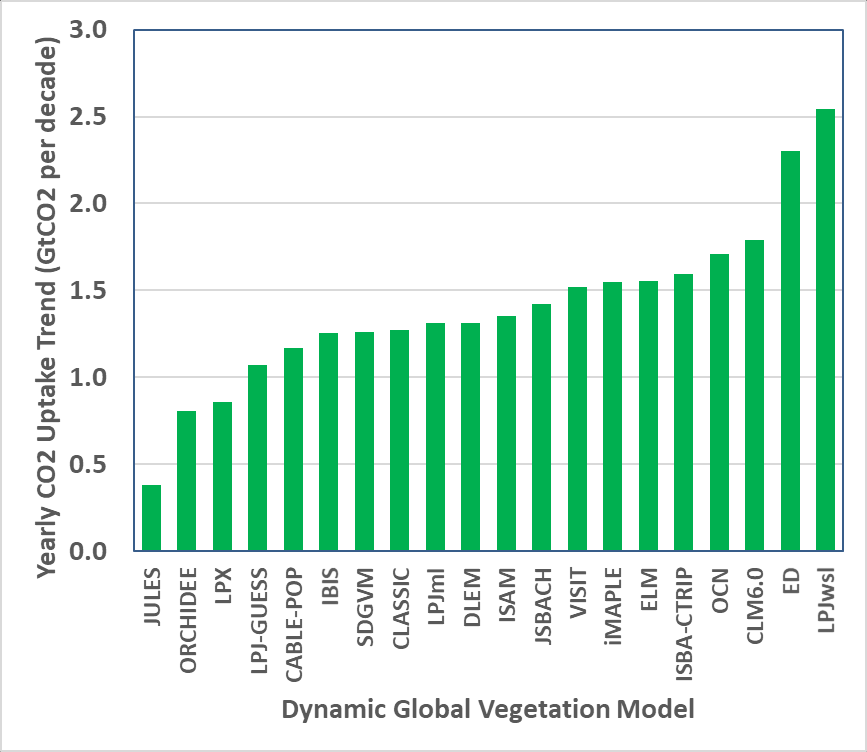
\includegraphics[width=1.0\textwidth]{bilder/bilderKlima-0013.png}\\[1cm]
\end{center}
\caption{Trends der jährlichen CO2-Aufnahme (GtCO2 pro Jahr und Jahrzehnt) durch Landprozesse
im Zeitraum 1959–2023, simuliert durch 20 verschiedene dynamische globale Vegetationsmodelle, die regelmäßig
vom Global Carbon Project (Friedlingstein, 2024) veröffentlicht werden.}
\end{figure}

\subsubsection*{CO$_2$-Aufnahme durch Landprozesse}
Die Aufnahme von zusätzlichem CO$_2$ aus der Atmosphäre durch Landoberflächenprozesse (wie auch aus der globalen Ergrünung geschlossen) wurde mit 20 verschiedenen dynamischen globalen Vegetationsmodellen modelliert, deren Ausgaben jährlich vom Global Carbon Project aktualisiert werden (Friedlingstein, 2024). Wie in Abb. 3.2.3 zu sehen ist, stimmen alle diese Modelle darin überein, dass Vegetation und Böden Kohlenstoff aus der Atmosphäre sequestriert haben. Aber wir sehen auch, dass die langfristigen Trends über 1959 bis 2023 (65 Jahre) stark zwischen den Modellen variieren, um fast einen Faktor von 7. Dies zeigt, dass erhebliche Unsicherheit darüber besteht, wie schnell Landprozesse CO$_2$ aus der Atmosphäre entfernen, was wiederum Unsicherheit in zukünftigen atmosphärischen CO$_2$-Konzentrationen schafft, die dann Unsicherheit in Klimamodellsimulationen zukünftiger Klimaveränderungen erzeugen.

\subsubsection*{CO$_2$-Aufnahme durch Ozeanprozesse}
Die Aufnahme von zusätzlichem CO$_2$ aus der Atmosphäre durch Ozeanprozesse wurde mit 10 verschiedenen Ozeanbiogeochemie-Modellen modelliert, deren Ausgaben jährlich vom Global Carbon Project aktualisiert werden (Friedlingstein, 2024). Wie die Ergebnisse der Landmodelle stimmen alle Ozeanmodelle darin überein, dass die globalen Ozeane während 1959-2023 Kohlenstoff aus der Atmosphäre mit einer steigenden Rate sequestriert haben (Abb. 3.2.4). Im Gegensatz zu den Landmodellen zeigen die Ozeanmodelle jedoch eine viel bessere Übereinstimmung miteinander, wobei das Modell mit der schnellsten steigenden CO$_2$-Aufnahme nur 65 Prozent schneller ist als das Modell mit der langsamsten steigenden CO$_2$-Aufnahme. Trotz der relativen Übereinstimmung zwischen den Modellen bemerkt Friedlingstein et al. (2022), dass es erhebliche Diskrepanzen zwischen den verschiedenen Methoden über die Stärke der Ozeansenke im letzten Jahrzehnt gibt, besonders im Südozean.
Beachten Sie, dass der durchschnittliche Trend in der CO$_2$-Aufnahme über alle Landmodelle in Abb. 3.2.3 25 Prozent größer ist als der durchschnittliche Trend in der Ozeanaufnahme. Dies deutet darauf hin, dass Landprozesse in ihrer Fähigkeit, CO$_2$ zu entfernen, schneller zunehmen als Ozeanprozesse ihre CO$_2$-Sequestrierung steigern.

\begin{figure}[H]
\begin{center}
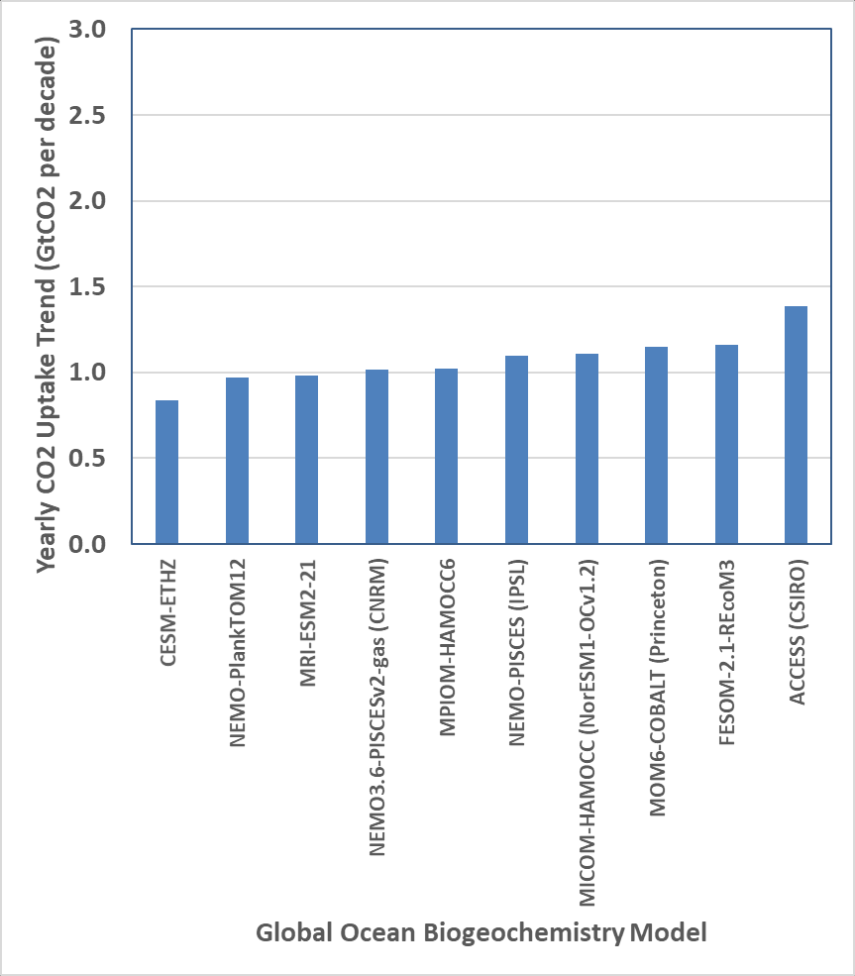
\includegraphics[width=1.0\textwidth]{bilder/bilderKlima-0015.png}\\[1cm]
\end{center}
\caption{Trends der jährlichen CO2-Aufnahme (GtCO2 pro Jahr und Jahrzehnt) durch Ozeanprozesse im Zeitraum
1959–2023, simuliert durch 10 verschiedene ozeanische Biogeochemie-Modelle, regelmäßig berichtet vom
Global Carbon Project (Friedlingstein, 2024).}
\end{figure}


\section{Urbanisierungseinfluss auf Temperaturtrends}
Historische Temperaturdaten über Land wurden hauptsächlich dort gesammelt, wo Menschen leben. Dies wirft das Problem auf, wie man nicht-klimatische Erwärmungssignale aufgrund von städtischen Wärmeinseln (UHI) und anderen Veränderungen der Landoberfläche herausfiltern kann. Wenn diese nicht entfernt werden, könnten die Daten beobachtete Erwärmung übermäßig Treibhausgasen zuschreiben. Das IPCC erkennt an, dass Rohtemperaturdaten mit UHI-Effekten kontaminiert sind, behauptet aber, Datenbereinigungsverfahren zu haben, die sie entfernen. Es ist eine offene Frage, ob diese Verfahren ausreichend sind.
AR6 spielte dieses Problem herunter, indem es sagte (WGI S. 235), dass keine neuen Beweise aufgetaucht seien, um die AR5-Feststellung zu ändern, dass Urbanisierung eine Aufwärtsverzerrung von nicht mehr als 10 Prozent im globalen Landerwärmungstrend verursacht. AR5 (WGI S. 189) zitierte ebenfalls die 10-Prozent-Obergrenze ohne Quellenangabe. AR4 (WGI S. 244) zitierte Jones et al. (1990) und Peterson et al. (1999) als Grundlage der Behauptung. Peterson et al. fanden keinen Unterschied in Trends zwischen ländlichen und städtischen Stichproben, obwohl ihre Definition von ländlich lokale Bevölkerungen bis zu 10.000 Personen einschloss, während der relative Einfluss der Urbanisierung deutlich darunter beginnt (Spencer et al., 2025). Jones et al. verglichen ländliche/städtische Erwärmung in drei Regionen: Ostaustralien, Ostchina und Westliche Sowjetunion. Ihre Definition von \emph{ländlich} umfasste Städte bis zu 10.000 in der ehemaligen Sowjetunion und bis zu 100.000 in China. Sie fanden relative Erwärmungsverzerrungen größer als 10 Prozent in diesen Gebieten, vermuteten aber, dass der Urbanisierungseffekt, gemittelt über die Gebiete, die sie nicht untersuchten, die globale Landverzerrung auf unter 10 Prozent des beobachteten Erwärmungstrends bringen würde.

Mehrere Arbeiten erschienen vor dem IPCC AR4, die argumentierten, dass der erwärmende Effekt von UHIs eine relativ große (30-50\%) Komponente zur beobachteten Erwärmung hinzufügte und nicht von Klimamodellen simuliert wurde (de Laat und Maurellis 2006, McKitrick und Michaels 2007). Diese Befunde basierten auf Korrelationen zwischen Orten maximaler Erwärmung über Land und Orten maximaler sozioökonomischer Entwicklung. AR4 behauptete (S. 244), dass diese Korrelationen ein Artefakt natürlicher atmosphärischer Zirkulationen waren und tatsächlich statistisch insignifikant, und verwarf die Befunde auf dieser Grundlage. Ihre Behauptung war kontrovers, weil sie ohne unterstützende Beweise präsentiert wurde. McKitrick (2010) und McKitrick und Nierenberg (2010) zeigten, dass die Berücksichtigung verschiedener vermuteter alternativer Erklärungen für die Korrelationen ihre Signifikanz nicht beeinflusste. AR5 (S. 189) räumte ein, dass AR4 \emph{keine expliziten Beweise} für seine Bewertung geliefert hatte und erkannte weiter auf der Grundlage dieser Arbeiten an, dass es \emph{signifikante Beweise für eine solche Kontamination der Aufzeichnung} gab, d.h. eine Erwärmungsverzerrung in der Landaufzeichnung. Wie bereits bemerkt, trugen sie jedoch an anderer Stelle im AR5-Bericht die AR4-Behauptung vor, dass es weniger als 10 Prozent der beobachteten Erwärmung seien. Außerdem gaben sie keine Warnung über die Verwendung der Landaufzeichnung für Klimamessungen, obwohl sie die Beweise für UHI-Kontamination einräumten. Kürzlich schätzten Soon et al. (2023) eine Urbanisierungsverzerrung in der nordhemisphärischen Landaufzeichnung über 1850-2018, die ausreicht, um den Trend in der gemischten Aufzeichnung von \SI{0.55}{\celsius} auf \SI{0.89}{\celsius} pro Jahrhundert zu erhöhen.

Einige Studien, die Beweise gegen UHI-Kontamination lieferten, verglichen Erwärmungsraten zwischen ländlichen und städtischen Standorten (Jones et al. 1990, Peterson et al. 1999, Wickham et al. 2013). Es ist nicht bekannt, ob solche Methoden UHI-Verzerrung erkennen könnten, selbst wenn sie vorhanden wäre. Der Einfluss der UHI-Erwärmung ist logarithmisch in der Bevölkerung, mit anderen Worten, er ist am stärksten bei niedriger Bevölkerungsdichte und flacht dann ab, wenn sich die lokale Urbanisierung ausdehnt (Oke 1973, Spencer et al. 2025). Daher beweist das Versagen, einen Unterschied in Erwärmungsraten zwischen städtischen und ländlichen Stationen zu finden, nicht die Abwesenheit von UHI-Kontamination. McKitrick (2013) lieferte eine empirische Demonstration, in der sich die ländlichen/städtischen Trends in einem Datensatz, der aus anderen Gründen als mit UHI-Verzerrung kontaminiert erwiesen wurde, nicht signifikant unterschieden.

Parker (2006) untersuchte eine Stichprobe städtischer Standorte und fand keinen Unterschied in Trends zwischen Untergruppen, die nach nächtlicher Windgeschwindigkeit unterteilt waren, und schloss auf dieser Grundlage, dass Urbanisierung kein signifikanter Faktor sein könnte. Auch hier ist die Frage, ob eine solche Methode UHI-Verzerrung finden würde, selbst wenn sie vorhanden wäre. McKitrick (2013) präsentierte ein Beispiel, in dem UHI-kontaminierte Daten keine signifikanten Trendunterschiede zeigten, wenn sie nach Windgeschwindigkeit stratifiziert wurden.

Die Herausforderung bei der Messung von UHI-Verzerrung besteht darin, lokale Temperaturveränderungen mit einer entsprechenden Veränderung in Bevölkerung oder Urbanisierung zu verknüpfen, anstatt mit einer statischen Klassifikationsvariable wie ländlich oder städtisch. Spencer et al. (2025) verwendeten neu verfügbare historische Bevölkerungsarchive, um eine solche Analyse durchzuführen, und fanden Beweise für signifikante UHI-Verzerrung in US-Sommertemperaturdaten.

Zusammenfassend, während es eindeutig Erwärmung in der Landaufzeichnung gibt, gibt es auch Beweise dafür, dass sie durch Urbanisierungsmuster nach oben verzerrt ist und dass diese Verzerrungen nicht vollständig durch die Datenverarbeitungsalgorithmen entfernt wurden, die zur Erstellung von Klimadatensätzen verwendet werden.

\vfill
\noindent\textbf{Literaturverzeichnis:}

\begingroup
\parindent=0pt
\everypar{\hangindent=2em\hangafter=1\relax}

Angert, A., S. Biraud, Bonfils, C., Buermann, W. and I. Fung (2004). CO2 seasonality indicates origins of
post-Pinatubo sink. Geophysical Research Letters 31. \url{https://doi.org/10.1029/2004GL019760}

AR6: Intergovernmental Panel on Climate Change Sixth Assessment Report (2021) Working Group I
Contribution. www.ipcc.ch.

AR5: Intergovernmental Panel on Climate Change Fifth Assessment Report (2013) Working Group I
Contribution. www.ipcc.ch.

AR4: Intergovernmental Panel on Climate Change Fourth Assessment Report (2007) Working Group I
Contribution. www.ipcc.ch.

Burgess, Matthew et al (2021) Environmental Research Letters 16 014016
\url{https://iopscience.iop.org/article/10.1088/1748-9326/abcdd2/meta}

Ciais, P., C. Sabine, G. Bala, L. Bopp, V. Brovkin,et al. (2013): Carbon and Other Biogeochemical Cycles.
In: Climate Change 2013: The Physical Science Basis. Contribution of Working Group I to the Fifth
Assessment Report of the Intergovernmental Panel on Climate Change [Stocker, T.F., D. Qin, G.-K.
Plattner, M. Tignor,et al. (eds.)]. Cambridge University Press, Cambridge, United Kingdom and New
York, NY, USA

Connolly, Roman, Willie Soon, Michael Connolly et al. (2021) How much has the Sun influenced
Northern Hemisphere temperature trends? An ongoing debate Research in Astronomy and
Astrophysics 21(6) doi: 10.1088/1674-4527/21/6/131 \url{https://iopscience.iop.org/article/10.1088/1674-
4527/21/6/131}

Crisp, David \& Dolman, Han (A.J.) \& Tanhua, Toste \& Mckinley, Galen \& Hauck, Judith \& Bastos, Ana
\& Sitch, Stephen \& Eggleston, Simon \& Aich, Valentin. (2022). How Well Do We Understand the
Land‐Ocean‐Atmosphere Carbon Cycle?. Reviews of Geophysics. 60. 10.1029/2021RG000736.

De Laat, A.T.J., and A.N. Maurellis (2006), Evidence for influence of anthropogenic surface processes on
lower tropospheric and surface temperature trends, International Journal of Climatology 26:897—913.

Friedlingstein, P., and 95 co-authors (2024): Global Carbon Budget 2024, Earth System Science Data
14(4), https://essd.copernicus.org/preprints/essd-2024-519

Hausfather et al. (2019) “Evaluating the Performance of Past Climate Model Projections” Geophysical
Research Letters 47(1) https://doi.org/10.1029/2019GL085378

Hausfather, Z. and G. Peters (2020a) “Emissions – the ‘business as usual’ story is misleading” Nature 29
January 2020 https://www.nature.com/articles/d41586-020-00177-3

Hausfather, Z. and G. Peters (2020b) RCP8.5 is a problematic scenario for near-term emissions.
Proceedings of the National. Academy of Sciences 117, 27791–27792 (2020)

Jenkins, S., Smith, C., Allen, M. et al. Tonga eruption increases chance of temporary surface temperature
anomaly above 1.5 °C. Nature Climate Change. 13, 127–129 (2023). https://doi.org/10.1038/s41558-
022-01568-2

Jones, P. D., P. Y. Groisman, M. Coughlan, N. Plummer, W.-C. Wang, and T. R. Karl (1990),
Assessment of urbanization effects in time series of surface air temperature over land, Nature, 347,
169 – 172

Liu, Pengfei et al. (2021) “Improved estimates of preindustrial biomass burning reduce the magnitude of
aerosol climate forcing in the Southern Hemisphere” Science Advances 7(22) May 2021
https://doi.org/10.1126/sciadv.abc1379

McKitrick, R.R. and P.J. Michaels (2007), Quantifying the influence of anthropogenic surface processes
and inhomogeneities on gridded global climate data, Journal of Geophysical Research, 112, D24S09,
doi:10.1029/2007JD008465.

McKitrick, Ross R. (2010) Atmospheric Oscillations Do Not Explain the Temperature-Industrialization
Correlation. Statistics Politics and Policy Vol 1. No. 1., July 2010

McKitrick, Ross R. (2013) Encompassing Tests of Socioeconomic Signals in Surface Climate
Data. Climatic Change doi 10.1007/s10584-013-0793-5. Volume 120, Issue 1-2.
http://link.springer.com/article/10.1007%2Fs10584-013-0793-5

McKitrick, Ross R. and Nicolas Nierenberg (2010) Socioeconomic Patterns in Climate Data. Journal of
Economic and Social Measurement, 35(3,4) pp. 149-175. DOI 10.3233/JEM-2010-0336

McKitrick, Ross R., Mark Strazicich and Junsoo Lee (2012) “Long-Term Forecasting of Global Carbon
Dioxide Emissions: Reducing Uncertainties Using a Per-Capita Approach.” Journal of
Forecasting, Vol 32, Issue 5, pp 435-451 DOI: 10.1002/for.2248.

Oke, T.R., 1973: City size and the urban heat island, Atmospheric Environment 7, 769-779

Parker, D.E. (2006) “A Demonstration that Large-Scale Warming is not Urban.” Journal of Climate
19:2882—2895.

Peterson, Thomas C., Kevin P. Gallo, Jay Lawrimore, Timothy W. Owen, Alex Huang, David A.
McKittrick (1999) Global rural temperature trends. Geophysical Research Letters February 1999
https://doi.org/10.1029/1998GL900322

Pielke Jr., Roger and Ritchie, Justin (2020) “Systemic Misuse of Scenarios in Climate Research and
Assessment” Social Sciences Research Network April 2020, available at:
https://ssrn.com/abstract=3581777

Pielke Jr, R., Burgess, M. G., \& Ritchie, J. (2022). Plausible 2005-2050 emissions scenarios project
between 2 and 3 degrees C of warming by 2100. Environmental Research Letters 17 024027
https://iopscience.iop.org/article/10.1088/1748-9326/ac4ebf/pdf

Scaffeta, Nicola, Richard C. Willson, Jae N. Lee and Dong Wu (2019) Modeling Quiet Solar Luminosity
Variability from TSI Satellite Measurements and Proxy Models during 1980–2018. Remote Sensing
11(21) 2569 https://doi.org/10.3390/rs11212569

Schoeberl, M.R., Y. Wang, G. Taha, D.J. Zawada, R. Ueyama and A. Dessler, 2024. Evolution of the
climate forcing during the two years after the Hunga Tonga-Hunga Ha’apai eruption. Journal of
Geophysical Research., 129.

Schwalm, C.R., S. Glendon, P. B. Duffy (2020) RCP8.5 tracks cumulative CO2 emissions. Proceedings of
the National Academy of Sciences U.S.A. 117, 19656–19657 (2020).

Soon,W.; Connolly, R.; Connolly, M.; Akasofu, S.-I.; Baliunas, S.; et al. (2023) The Detection and
Attribution of Northern Hemisphere Land Surface Warming (1850–2018) in Terms of Human and
Natural Factors: Challenges of Inadequate Data. Climate 2023, 11, 179.
https://doi.org/10.3390/cli11090179

Spencer, Roy W, John R Christy and William D. Braswell (2025) Urban Heat Island Effects in U.S.
Summer Surface Temperature Data, 1895–2023 Journal of Applied Meteorology and Climatology
April 2025 https://doi.org/10.1175/JAMC-D-23-0199.1

Wickham C, R Rohde , RA Muller, J Wurtele, J Curry, et al. (2013) Influence of Urban Heating on the
Global Temperature Land Average using Rural Sites Identified from MODIS Classifications.
Geoinformatics and Geostatistics: An Overview 1:2.

Zacharias, Pia (2014) An Independent Review of Existing Total Solar Irradiance Records. Surveys in
Geophysics 35 pp. 897—912 https://link.springer.com/article/10.1007/s10712-014-9294-y
\endgroup

\cleardoublepage
\chapter*{TEIL II: KLIMAREAKTION AUF CO$_2$-EMISSIONEN}
%\numberwithin{figure}{chapter}
\FigureNumbersByChapter
\addcontentsline{toc}{chapter}{TEIL II: KLIMAREAKTION AUF CO$_2$-EMISSIONEN}
\cleardoublepage
\chapter{Klimasensitivität bezüglich CO$_2$-Einwirkung}
\paragraph{Kapitelzusammenfassung}
\begin{quote}
Es gibt eine wachsende Erkenntnis, dass Klimamodelle nicht für den Zweck geeignet sind, die Gleichgewichts-Klimasensitivität (ECS) des Klimas gegenüber steigendem CO$_2$ zu bestimmen. Das IPCC hat sich datengetriebenen Ansätzen zugewandt, einschließlich historischer Daten und paläoklimatischer Rekonstruktionen, aber deren Zuverlässigkeit ist durch Datenmängel beeinträchtigt.
Datengetriebene ECS-Schätzungen tendieren dazu, niedriger zu sein als klimamodell-generierte Werte. Die obere Grenze des IPCC AR6 für den wahrscheinlichen ECS-Bereich beträgt \SI{4.0}{\celsius}, niedriger als der AR5-Wert von \SI{4.5}{\celsius}. Diese Senkung der oberen Grenze scheint durch paläoklimatische Daten gut begründet zu sein. Die untere Grenze des AR6 für den wahrscheinlichen ECS-Bereich beträgt \SI{2.5}{\celsius}, wesentlich höher als der AR5-Wert von \SI{1.5}{\celsius}. Diese Erhöhung der unteren Grenze ist weniger gerechtfertigt; Belege seit AR6 zeigen, dass die untere Grenze des wahrscheinlichen Bereichs bei etwa \SI{1.8}{\celsius} liegt.
\end{quote}
\section{Einleitung}
Das Ausmaß der Klimareaktion auf steigende CO$_2$-Konzentrationen steht im Zentrum der wissenschaftlichen Debatte über den anthropogenen Klimawandel und damit auch der öffentlichen Debatte über \emph{Klimaschutzmaßnahmen}. Das einfachste Maß für diese Reaktion ist der Anstieg der globalen durchschnittlichen Oberflächentemperatur, quantifiziert durch die Gleichgewichts-Klimasensitivität (ECS). ECS ist definiert als das Ausmaß der Erwärmung, das als Reaktion auf eine Verdoppelung von CO$_2$ von seiner vorindustriellen Konzentration von \SI{280}{ppm} erwartet wird, nachdem alle Klimakomponenten Zeit hatten, sich anzupassen. Einige Komponenten, wie die Temperaturen in der unteren Atmosphäre (Troposphäre), passen sich schnell an, während andere wie der tiefe Ozean und die Kryosphäre möglicherweise jahrhundertelang brauchen. Ein verwandtes Maß, die Transiente Klimareaktion (TCR), beschreibt die kürzeren Zeitskalen besser; sie ist definiert als das Ausmaß der Erwärmung, wenn die CO$_2$-Konzentration durch einen jährlichen Anstieg von einem Prozent über 70 Jahre verdoppelt wird.

Der Charney-Bericht von 1979 für die U.S. National Academy of Sciences (National Research Council 1979) schlug vor, dass die wahrscheinlichste ECS \SI{3.0}{\celsius} $\pm$ \SI{1.5}{\celsius} sei. Das IPCC bekräftigte diesen Bereich wiederholt mit nur geringfügigen Variationen bis zu seinem jüngsten AR6. AR5 bezeichnete \SIrange{1.5}{4.5}{\celsius} als den wahrscheinlichen Bereich (66 Prozent Wahrscheinlichkeit) und stellte fest, dass ECS extrem unwahrscheinlich (95 Prozent Wahrscheinlichkeit) unter \SI{1.0}{\celsius} und sehr unwahrscheinlich (90 Prozent Wahrscheinlichkeit) über \SI{6.5}{\celsius} liegt.

Die Unsicherheit in ECS ist hartnäckig weit geblieben, trotz vieler einzelner Studien, die behaupteten, sie zu verringern (Hausfather 2023). Zuletzt verengte AR6 den wahrscheinlichen Bereich auf \SIrange{2.5}{4.0}{\celsius} und betrachtete den sehr wahrscheinlichen Bereich als \SIrange{2.0}{5.0}{\celsius}. Diese Verengung am unteren Ende wird bestritten, wie unten diskutiert wird.

Unsicherheiten in ECS sind höchst folgenreich für die Politikgestaltung. Wie in Kapitel 11 diskutiert wird, verwenden Wirtschaftsmodelle ECS-Werte, um die Kosten von CO$_2$-Emissionen zu projizieren. Der traditionelle Wert (\SI{3.0}{\celsius}) hat typischerweise bescheidene globale soziale Kosten von CO$_2$-Emissionen ergeben, ausreichend um einige politische Maßnahmen zu rechtfertigen, aber meist auf später in diesem Jahrhundert verschoben. Wenn ECS sehr hoch ist (über \SI{4.5}{\celsius}), werden sofortige aggressive Emissionskontrollen zwingender, während keine CO$_2$-Emissionskontrollen wirtschaftlich gerechtfertigt sind für ECS unter \SI{2.0}{\celsius} (Dayaratna et al. 2017, 2020). Eine präzise Schätzung zu erhalten ist unmöglich, daher muss die Politikgestaltung die Unsicherheit berücksichtigen.

Für sich allein ist der Gleichgewichts-Erwärmungseffekt einer Verdoppelung des atmosphärischen CO$_2$ etwas mehr als \SI{1}{\celsius} (Soden und Held 2006). Größere Werte von ECS entstehen durch positive Rückkopplungen, die die CO$_2$-Erwärmung verstärken. Wasserdampf-Rückkopplung ist positiv: eine wärmere Atmosphäre könnte mehr Wasserdampf haben, der selbst ein starkes Treibhausgas ist. Wärmere Temperaturen führen auch zu weniger Schnee- und Meereisbedeckung, wodurch die Erde mehr von der Sonnenstrahlung absorbieren kann. Einige einfache Schätzungen dieser Rückkopplungen erhöhen die ECS auf etwa \SI{2}{\celsius} (Sherwood et al., 2020). Größere Werte von ECS sind mit positiven Wolken-Rückkopplungen verbunden.

Klimawissenschaftler verwenden mehrere Beweislinien, um die Gleichgewichts-Klima\-sensitivität zu bestimmen:
\begin{itemize}
\item  Klimamodell-Simulationen
\item  Historische Beobachtungen  
\item  Paläoklimatische Rekonstruktionen
\item  Prozessverständnis von Rückkopplungen
\end{itemize}

\section{Modellbasierte Schätzungen der Klimasensitivität}
Die in IPCC AR4 und AR5 angegebenen ECS-Bereiche wurden hauptsächlich durch die Untersuchung des Verhaltens großmaßstäblicher Klimamodelle, auch General Circulation Models (GCMs) genannt, erhalten. Das IPCC änderte jedoch den Kurs in seinem AR6, als es sich einer direkteren datengetriebenen Methodik zuwandte. Hier diskutieren wir einige der Fallstricke bei der Verwendung von GCMs, um die Klimasensitivität der Erde zu bestimmen.

ECS kann aus Klimamodell-Simulationen bestimmt werden, indem die CO$_2$-Konzentration verdoppelt und mehrere Jahrhunderte für die Erwärmung zum Gleichgewicht ermöglicht werden. Um die Notwendigkeit solch langer Simulationen zu vermeiden, wird \emph{effektive Klimasensitivität} üblicherweise aus einer 150-Jahres-Simulation als Reaktion auf eine plötzliche Vervierfachung von CO$_2$ bewertet.

Im Prinzip ist ECS eine emergente Eigenschaft von GCMs –- das heißt, sie wird nicht direkt parametrisiert oder abgestimmt, sondern entsteht vielmehr in den Ergebnissen der Simulation. Anderweitig plausible GCMs und Parameterauswahlen wurden verworfen wegen wahrgenommener Konflikte mit einer erwarteten Erwärmungsrate oder Abneigung gegen eine Klimasensitivität des Modells außerhalb eines akzeptierten Bereichs (Mauritsen et al. 2012). Diese Praxis war für die in AR4 verwendeten Modelle üblich; Modellierer sind mit der Zeit von dieser Praxis abgekommen. Jedoch, selbst in einem CMIP6-Modell, stellen Mauritsen und Roeckner (2020) das Folgende bezüglich ihres Max-Planck-Institut (MPI) Klimamodells fest (Hervorhebung hinzugefügt):

\begin{quote}
Wir haben dokumentiert, wie wir das globale Klimamodell MPI-ESM1.2 abstimmten, um der instrumentellen Aufzeichnung der Erwärmung zu entsprechen; ein Unterfangen, das eindeutig erfolgreich war. Aufgrund der historischen Reihenfolge der Ereignisse war die Wahl, dies praktisch zu tun, indem eine ECS von etwa 3 K mittels Wolken-Rückkopplungen anvisiert wurde, anstatt die Aerosol-Forcierung abzustimmen.  
\end{quote}

Mit anderen Worten, die MPI-Modellierer wählten einen ECS-Wert von \SI{3}{\celsius} und stimmten dann die Wolken-Parametrisierungen ab, um ihr beabsichtigtes Ergebnis zu erreichen.

Wie bemerkt, ist die direkte Erwärmung durch CO$_2$-Verdoppelung nur etwa \SI{1}{\celsius} (Soden und Held 2006); weitere Erwärmung entsteht durch Klima-Rückkopplungen, die nicht explizit vom GCM aufgelöst werden, sondern auf Parametrisierungen physikalischer Prozesse angewiesen sind. Höhere Werte von ECS entstehen primär durch positive Wolken-Rückkopplungen, während das Ausmaß und sogar das Vorzeichen der Rückkopplungen sehr unsicher sind. Elemente der Wolken-Rückkopplung umfassen Änderungen in der Breitenverteilung von Wolken, Änderungen in der Verteilung der Wolkenhöhe (Änderungen in niedrigen versus hohen Wolken), Änderungen in der Phase von Wolken (Eis versus Flüssigkeit), Änderungen in der Wolkenpartikelgröße (verbunden mit Änderungen in Konzentration und/oder Zusammensetzung von Aerosolpartikeln), Änderungen in der Niederschlagseffizienz von Wolken, und sogar Änderungen darin, wie Wolken über den täglichen Sonnenzyklus verteilt sind (Curry und Webster, 1999). Es ist für GCMs schwierig, irgendeinen dieser Prozesse aufgrund ihrer kleinen Skala korrekt zu simulieren, geschweige denn vorherzusagen, wie sie sich in der Zukunft ändern werden. Weiterhin modulieren Wolkenprozesse die Größenordnungen der Wasserdampf-, Lapse-Rate- und Oberflächenalbedo-Rückkopplungen.

\begin{figure}[H]
\begin{center}
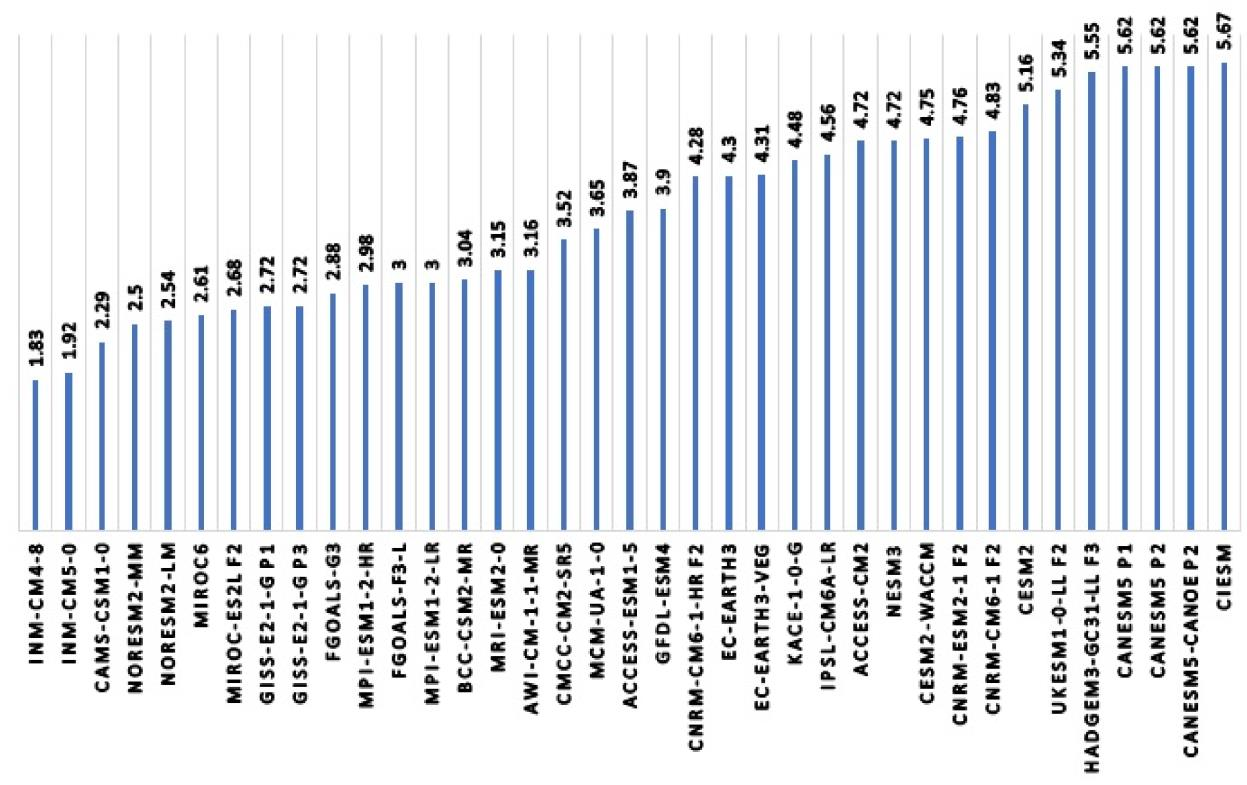
\includegraphics[width=1.0\textwidth]{bilder/bilderKlima-0017.jpg}\\[1cm]
\end{center}
\caption{Gleichgewichtsklimasensitivitäten in °C von 37 Klimamodellen aus dem CMIP6-Ensemble.
Die Kennungen für die verschiedenen Modelle sind auf der horizontalen Achse angegeben. Aus (Scafetta, 2021)}
\end{figure}


Die Spannweite der ECS-Werte aus dem CMIP5-Ensemble von Klimamodellen, die in AR5 verwendet wurden, war \SIrange{2.0}{4.7}{\celsius}; dieser Bereich vergrößerte sich für die CMIP6-Modelle, die in AR6 verwendet wurden, auf zwischen $1.8$ und \SI{5.7}{\celsius} (Chen et al., 2021, Scaffeta 2021, siehe Abbildung 4.1). Weit davon entfernt, die modellbasierte Klimasensitivität aufzulösen, scheint sich der Bereich zu vergrößern. Die Hauptursache der gesamten Aufwärtsverschiebung in ECS in CMIP6 relativ zu CMIP5 ist eine größere positive Wolken-Rückkopplung, angetrieben durch Änderungen in den Wolken-Parametrisierungen in vielen CMIP6-Modellen (Zelinka et al., 2020).

Aufgrund von Bedenken über Modellabstimmung und die hohe Empfindlichkeit gegenüber Wolken-Parametrisierungen stützte sich AR6 (2021) nicht auf Klimamodell-Simulationen in ihrer Bewertung der Klimasensitivität, sondern verließ sich stattdessen auf datengetriebene Methoden.

\section{Datengetriebene Schätzungen der Klimasensitivität}
Klimasensitivität kann auch aus instrumentellen Aufzeichnungen von Oberflächentemperaturen und ozeanischem Wärmeinhalt geschätzt werden, kombiniert mit Schätzungen darüber, wie sich Klimaforcierungen (z.B. Treibhausgase, solar, Vulkane, Aerosole) in der Vergangenheit verändert haben (Otto et al., 2013). Mit dieser Information kann ein einfaches empirisches Energiebilanz-Modell eingesetzt werden. Es erfordert die Schätzung eines Rückkopplungsparameters, dessen Unsicherheiten in der resultierenden ECS stark verstärkt werden (Roe und Baker, 2007).

Die Genauigkeit der datengetriebenen Methoden hängt von der Qualität der Eingangsdaten ab. Annahmen sind über ozeanische Wärmespeicherung nötig, und gute Daten sind nur für die letzten Jahrzehnte verfügbar. Die größte Quelle der Unsicherheit ist die Menge und Zusammensetzung von Aerosolpartikeln und ihre Wechselwirkungen mit Wolkenstrahlungseigenschaften (der sogenannte indirekte Aerosoleffekt; siehe Abbildungen 3.1.1, 3.1.2). Klimamodelle zeigen Erwärmung als Reaktion auf THG, aber Abkühlung als Reaktion auf Aerosole (Schwartz et al., 2007). Beobachtete Erwärmung des 20. Jahrhunderts kann gezeigt werden, dass sie konsistent ist entweder mit niedriger ECS und niedriger Aerosol-Abkühlung, oder hoher ECS und hoher Aerosol-Abkühlung. Da die Verwendung fossiler Brennstoffe sowohl THG als auch Aerosole zur Atmosphäre hinzufügt, müssen beide Effekte geschätzt werden, um den Erwärmungseffekt von CO$_2$ zu isolieren.

Paläoklima-Proxies werden auch verwendet, um die Sensitivität vergangener Klimate zu bewerten, indem paläoklimatische Änderungen in den Erdtemperaturen mit Schätzungen von Änderungen in Forcierungen verglichen werden. Die zwei informativsten Perioden sind das letzte glaziale Maximum (vor etwa 20.000 Jahren), das etwa \SIrange{3}{7}{\celsius} kälter war als heute, und eine mittlere Pliozän-Periode (vor etwa drei Millionen Jahren), die \SIrange{1}{3}{\celsius} wärmer war als heute. Die Grenzen der Abkühlung während des letzten glazialen Maximums geben den besten einzelnen Beweis, dass hohe Werte der Klimasensitivität unwahrscheinlich sind. Jedoch sind paläoklimatische Schätzungen mit sehr großen Unsicherheiten in den geschätzten Temperaturen und Forcierungen verbunden. Weiterhin könnten Schätzungen der Klimasensitivität basierend auf vergangenen Klimazuständen nicht auf den aktuellen Zustand des Klimasystems anwendbar sein.

Ein wiederkehrendes Thema in der Klimaliteratur ist, dass ECS-Schätzungen basierend auf historischen Daten kleiner sind als ECS-Schätzungen, die aus Klimamodellen abgeleitet werden (Sherwood und Forest 2024). Etwa 15 Schätzungen basierend auf historischen Daten erschienen in der begutachteten Literatur zwischen 2012 und 2024, die ECS-Bestschätzungen zwischen \SI{1.0}{\celsius} und \SI{2.5}{\celsius} ergaben, obwohl Kritiker einige der Methoden und die Datenqualität in Frage gestellt haben. Für AR6 legte das IPCC primäres Gewicht auf die Ergebnisse von Sherwood et al. (2020), die historische Daten und paläoklimatische Proxies mit dem prozessbasierten Ansatz kombinierten und eine Bestschätzung von \SI{3.1}{\celsius} mit einem wahrscheinlichen Bereich von \SIrange{2.6}{3.9}{\celsius} ergaben. Lewis (2022) äußerte eine Reihe von Bedenken über dieses Ergebnis, einschließlich methodologischer Fehler, veralteter Eingangswerte und der Verwendung subjektiver Bayesscher Priors in der Analyse. Lewis' Analyse fand, dass Klimasensitivität geschätzt wird, viel niedriger und besser eingegrenzt zu sein als in der Sherwood et al. Analyse – Median \SI{2.2}{\celsius} (\SIrange{1.8}{2.7}{\celsius} im $17-83$ Prozent wahrscheinlichen Bereich, und \SIrange{1.6}{3.2}{\celsius} im $5-95$ Prozent sehr wahrscheinlichen Bereich). Das IPCC AR6 schätzte nur eine $5$ Prozent Wahrscheinlichkeit, dass ECS unter \SI{2.3}{\celsius} lag, während Lewis es auf über $50$ Prozent schätzte. Die jüngsten Veröffentlichungen in der Debatte zwischen Sherwood et al. und Lewis verteidigen weiterhin ihre jeweiligen Positionen: Sherwood und Foster (2024) und Lewis (2025).

Ein in AR6 betontes Argument ist, dass datengetriebene ECS-Schätzungen die zukünftige Erwärmungsreaktion auf THG unterschätzen könnten wegen eines sogenannten \emph{Mustereffekts} (Forster et al., 2021). Es wird geglaubt, dass der tropische Pazifik die Gesamteffizienz, mit der die Erde Wärme in den Weltraum abstrahlt, stark beeinflusst, aber einige Regionen entfernen Wärme effizienter als andere. Wenn der West-Ost-Temperaturgradient im tropischen Pazifik in einem sich erwärmenden Klima geschwächt wird, würde sich die Erwärmung dort konzentrieren, wo Wärme weniger effizient entfernt wird, was ECS erhöht.

Die meisten Klimamodelle simulieren, dass steigende THG den West-Ost-Temperatur\-gradienten schwächen werden, was das IPCC in AR6 zu dem Schluss führte, dass datengetriebene ECS-Schätzungen den zukünftigen ECS-Wert unterschätzten. Jedoch wiesen Seager et al. (2019) darauf hin, dass, entgegen den Modellen, sich der West-Ost-Temperaturgradient über die Zeit verstärkt hat. Sie argumentierten weiter, dass der Mechanismus, der anderes in Klimamodellen vorhersagt, auf einer fehlerhaften Charakterisierung ozeanischer Dynamik basierte und es keinen Grund gibt zu erwarten, dass sich der Gradient schwächt. Ein ähnliches Argument wurde kürzlich von Lee et al. (2024) gemacht, die schlossen, dass \emph{die Trajektorie des beobachteten Trends die Reaktion auf zunehmende THG-Belastung in der Atmosphäre widerspiegelt}; mit anderen Worten, THG-Erwärmung sollte zu einer zukünftigen Verstärkung statt einer Schwächung des Temperaturgradienten führen. Erhöhte Effizienz der atmosphärischen Abkühlung impliziert, wenn überhaupt, dass die zukünftige ECS in einem sich erwärmenden Klima niedriger sein könnte als aktuelle Schätzungen.

\section{Transiente Klimareaktion}
Die Transiente Klimareaktion (TCR) bietet eine nützlichere Beobachtungseinschränkung für die Klimasensitivität. TCR ist der globale Temperaturanstieg, der entsteht, wenn CO$_2$ mit einer jährlichen Rate von 1 Prozent über einen Zeitraum von 70 Jahren erhöht wird (d.h. allmählich verdoppelt). Im Vergleich zur ECS vermeiden beobachtungsbasiert bestimmte Werte von TCR die Probleme von Unsicherheiten in der ozeanischen Wärmeaufnahme und der unscharfen Grenze bei der Definition des Gleichgewichts, die aus einer Reihe von Zeitskalen für die längerfristigen Rückkopplungsprozesse (z.B. Eisschilde) entstehen. TCR ist durch historische Erwärmung besser eingegrenzt als ECS. AR6 beurteilte den sehr wahrscheinlichen Bereich von TCR als \SIrange{1.2}{2.4}{\celsius}. Im Gegensatz zu ECS ist die obere Grenze von TCR enger eingegrenzt. Zum Vergleich: die von Lewis (2023) bestimmten TCR-Werte liegen bei $1.25$ bis \SI{2.0}{\celsius}, was eine viel bessere Übereinstimmung mit AR6-Werten zeigt, als beim Vergleich der ECS-Werte zu sehen war.

\vfill
\noindent\textbf{Literaturverzeichnis:}

\begingroup
\parindent=0pt
\everypar{\hangindent=2em\hangafter=1\relax}

Carbon Brief. (2020, July 22). Explainer: How scientists estimate climate sensitivity.
\url{https://www.carbonbrief.org/explainer-how-scientists-estimate-climate-sensitivity}

Carbon Brief. (2020, July 22). Guest post: Why low-end ‘climate sensitivity’ can now be ruled out.
\url{https://www.carbonbrief.org/guest-post-why-low-end-climate-sensitivity-can-now-be-ruled-out}

Carbon Brief. (2021, August 9). In-depth Q\&A: The IPCC’s sixth assessment report on climate science.
\url{https://www.carbonbrief.org/in-depth-qa-the-ipccs-sixth-assessment-report-on-climate-science}

Chen, D., et al. (2021). Framing, context, and methods. In V. Masson-Delmotte et al. (Eds.), Climate
change 2021: The physical science basis. Contribution of Working Group I to the Sixth Assessment
Report of the Intergovernmental Panel on Climate Change. Cambridge University Press.

Curry, J. A., \& Webster, P. J. (1999). Thermodynamic feedbacks in the climate system. In
Thermodynamics of atmospheres and oceans (pp. 351–385). Academic Press.

Dayaratna, Kevin, Ross McKitrick and David Kreutzer (2017) Empirically-Constrained Climate Sensitivity
and the Social Cost of Carbon. Climate Change Economics April 2017 DOI:
http://dx.doi.org/10.1142/S2010007817500063

Dayaratna, Kevin, Ross McKitrick and Patrick J. Michaels (2020) Climate Sensitivity, Agricultural
Productivity and the Social Cost of Carbon in FUND. Environmental Economics and Policy Studies
https://doi.org/10.1007/s10018-020-00263-w

Forster, P., et al. (2021). The Earth's energy budget, climate feedbacks, and climate sensitivity. In V.
Masson-Delmotte et al. (Eds.), Climate change 2021: The physical science basis. Contribution of
Working Group I to the Sixth Assessment Report of the Intergovernmental Panel on Climate Change.
Cambridge University Press.

Hausfather, Z. (2020, July 22). Explainer: How scientists estimate climate sensitivity. Carbon Brief.
https://www.carbonbrief.org/explainer-how-scientists-estimate-climate-sensitivity

Lan, X., Tans, P., \& Thoning, K. W. (2025). Trends in globally-averaged CO$_2$ determined from NOAA
Global Monitoring Laboratory measurements. NOAA Global Monitoring Laboratory.
https://doi.org/10.15138/9N0H-ZH07

Lee, S., Byrne, M. P., Loikith, P. C., \& O’Dell, C. W. (2024). Zonal contrasts of the tropical Pacific
climate predicted by a global constraint. Climate Dynamics, 62(1–2), 229–246.
https://doi.org/10.1007/s00382-023-06741-7

Lewis, N. (2023). Objectively combining climate sensitivity evidence. Climate Dynamics, 61(9–10),
3155–3163. https://doi.org/10.1007/s00382-022-06398-8

Lewis, N. (2025). Comment on “Can uncertainty in climate sensitivity be narrowed further?” by
Sherwood and Forest (2024). EGUsphere [preprint]. https://doi.org/10.5194/egusphere-2025-1179

Thorsten Mauritsen et al., (2012) “Tuning the Climate of a Global Model,” Journal of Advances in
Modeling Earth Systems 4, no. 3 https://doi. org/10.1029/2012ms000154


Mauritsen, T., \& Roeckner, E. (2020). Tuning the MPI-ESM1.2 global climate model to improve the
match with instrumental record warming by lowering its climate sensitivity. Journal of Advances in
Modeling Earth Systems, 12, e2019MS002037. https://doi.org/10.1029/2019MS002037

Otto, A., Otto, F. E. L., Boucher, O., Church, J., Hegerl, G., Forster, P. M., Gregory, J. M., \& Johnson, G.
C. (2013). Energy budget constraints on climate response. Nature Geoscience, 6(6), 415–416.
https://doi.org/10.1038/ngeo1836

Pachauri, R. K., \& Meyer, L. (Eds.). (2015). Climate change 2014: Synthesis report. Intergovernmental
Panel on Climate Change.

Roe, G. and M. Baker (2007). Why is climate sensitivity so unpredictable? Science 318, 629-632.
https://doi.org/10.1126/science.1144735

Scafetta, N. (2021). Testing the CMIP6 GCM simulations versus surface temperature records from 1980–
1990 to 2011–2021: High ECS is not supported. Climate, 9(11), 161.
https://doi.org/10.3390/cli9110161

Schwartz, S. E., R. J. Charlson, H. Rodhe (2007). Quantifying climate change—Too rosy a picture?
Nature Climate Change 1, 23–24, https://doi.org/10.1038/climate.2007.22

Seager, R., Cane, M., Ting, M., Naik, N., Clement, A., DiNezio, P., \& Lee, D. E. (2019). Strengthening
tropical Pacific zonal sea surface temperature gradient consistent with rising greenhouse gases.
Nature Climate Change, 9(7), 517–522. https://doi.org/10.1038/s41558-019-0505-x

Sherwood, S. C., \& Forest, C. E. (2024). Opinion: Can uncertainty in climate sensitivity be narrowed
further? Atmospheric Chemistry and Physics, 24(5), 2679–2686. https://doi.org/10.5194/acp-24-2679-
2024

Sherwood, S. C., Bony, S., Boucher, O., Bretherton, C. S., Forster, P. M., Gregory, J. M., \& Stevens, B.
(2020). An assessment of Earth's climate sensitivity using multiple lines of evidence. Reviews of
Geophysics, 58(4). https://doi.org/10.1029/2019rg000678

Soden, B. J., and I.M. Held (2006). An assessment of climate feedbacks in coupled ocean–atmosphere
models. Journal of Climate, 19(14), 3354–3360. https://doi.org/10.1175/jcli3799.1

Zelinka, M. D., Myers, T. A., McCoy, D. T., Po-Chedley, S., Caldwell, P. M., Ceppi, P., Klein, S. A., \&
Taylor, K. E. (2020). Causes of higher climate sensitivity in CMIP6 models. Geophysical Research
Letters, 47, e2019GL085782. https://doi.org/10.1029/2019GL085782
\endgroup

\cleardoublepage
%\numberwithin{figure}{chapter}
\chapter{DISKREPANZEN ZWISCHEN MODELLEN UND INSTRUMENTELLEN BEOBACHTUNGEN}
\paragraph{Kapitelzusammenfassung}
\begin{quote}
Klimamodelle zeigen Erwärmungsverzerrungen in vielen Aspekten ihrer Reproduktion der vergangenen mehreren Jahrzehnte. Als Reaktion auf geschätzte Änderungen in der Forcierung produzieren sie zu viel Erwärmung an der Oberfläche (außer in den Modellen mit niedrigster ECS), zu viel Erwärmung in der unteren und mittleren Troposphäre und zu viel Verstärkung der Erwärmung in der Höhe.
Klimamodelle produzieren auch zu viel jüngste stratosphärische Abkühlung, ungültige hemisphärische Albedos, zu viel Schneeverlust und zu viel Erwärmung im Corn Belt. Das IPCC hat einige dieser Probleme anerkannt, aber nicht alle.
\end{quote}

\section{Einleitung}
Klimamodelle sind das primäre Werkzeug, das verwendet wird, um zukünftige Klimaänderungen als Reaktion auf steigende atmosphärische Konzentrationen anthropogener Treibhausgase zu projizieren. Um die Eignung von Klimamodellen für diesen Zweck zu bewerten, ist es vernünftig zu fragen, wie gut sie das aktuelle Klima und seine Variationen über das vergangene Jahrhundert reproduzieren. Der Kasten "Klimamodellierung" gibt einige Details darüber, wie Klimamodelle funktionieren.

Von großer Sorge ist die Tatsache, dass nach mehreren Jahrzehnten des Klimamodellierungsunternehmens mit etwa drei Dutzend Modellen, die von Forschungszentren auf der ganzen Welt betrieben werden, sich der Bereich zukünftiger Erwärmung, den sie als Reaktion auf eine hypothetische Verdoppelung des atmosphärischen CO$_2$ produzieren, über einen Faktor von drei erstreckt, wie wir im vorherigen Kapitel diskutiert haben. Dieser Bereich der Meinungsverschiedenheit zwischen Modellen hat seit Jahrzehnten nicht abgenommen.
Probleme mit Klimamodellen liegen nicht nur in ihrer Meinungsverschiedenheit über die Zukunft, sondern auch in ihrer Fähigkeit, die jüngste Vergangenheit zu replizieren. Hier überprüfen wir einige der wichtigsten Metriken der Klimamodell-Genauigkeit: Fähigkeit, historische Oberflächen-, troposphärische und stratosphärische Temperaturtrends zu reproduzieren; Fähigkeit, das vertikale Erwärmungsprofil zu reproduzieren; und Fähigkeit, andere Klimamerkmale wie Schneefall zu reproduzieren. In allen Fällen ist ein persistenter Befund, dass Modelle im Durchschnitt auf der Seite von zu viel Erwärmung als Reaktion auf geschätzte historische Forcierungen irren.


\begin{fullbox}{BOX: Klimamodellierung}
% --- Oberer (fließender) Teil: darf über mehrere Seiten laufen ---
Alle bis auf die einfachsten Klimamodelle repräsentieren die Erdoberfläche mit einem Gitter von Quadraten mit etwa 100 km Breite. Um die Atmosphäre zu simulieren, werden typischerweise 30 oder mehr Gitterboxen über diese Quadrate gestapelt. Der Ozean wird mit einem ähnlichen, aber feineren Gitter modelliert, was zu zehn Millionen von Gitterboxen für die Atmosphäre und Ozeane führt.

Die Computermodelle, basierend auf physikalischen Gesetzen, berechnen, wie sich Luft, Wasser und Energie zwischen Gitterboxen über die Zeit bewegen. Der Zeitschritt kann so klein wie 10 Minuten sein, und die Wiederholung dieses Prozesses Millionen von Malen ermöglicht die Simulation von Klima über Jahrhunderte. Das Ausführen dieser Modelle, selbst auf den leistungsstärksten Supercomputern, kann Monate dauern. Der Vergleich von Simulationsergebnissen mit historischen Klimadaten hilft, die Genauigkeit eines Modells zu bewerten, während Projektionen in die Zukunft Klimaänderungen unter angenommenen menschlichen und natürlichen Einflüssen schätzen.

Trotz der scheinbaren Einfachheit ist Klimamodellierung höchst komplex. Viele kritische Prozesse treten auf Skalen statt, die kleiner sind als die Gittergröße. Zum Beispiel hängen die Flüsse von Sonnenlicht und Wärme in der Atmosphäre stark von der Wolkenbedeckung ab. Da das Verfolgen einzelner Wolken unpraktisch ist, müssen Forscher "Subgitter"-Annahmen über die Verteilung von Wolken in jeder Gitterbox machen. Schnee- und Eisbedeckung, die beeinflusst, wie viel Sonnenlicht von der Oberfläche reflektiert oder absorbiert wird, ist ein weiterer Subgitter-Faktor.

Jede Subgitter-Annahme erfordert numerische Parameter, die sorgfältig gesetzt werden müssen. Modellierer schätzen diese Parameter zunächst basierend auf Physik und beobachteten Klimamustern, dann führen sie das Modell aus. Weil frühe Ergebnisse oft erheblich von realen Beobachtungen abweichen, \emph{stimmen} sie diese Parameter ab, um beobachtete Klimamerkmale besser zu entsprechen. Verschiedene Modellierungsteams verwenden unterschiedliche Annahmen und Abstimmungsstrategien, was zu verschiedenen Ergebnissen führt. Abstimmung ist ein notwendiger, aber delikater Aspekt der Klimamodellierung, wie bei jedem komplexen System. Schlechte Abstimmung kann zu ungenauen Simulationen führen, während übermäßige Abstimmung das Risiko birgt, Ergebnisse künstlich zu vorbestimmten Schlussfolgerungen zu lenken.

Die Spannweite der Modellrepräsentationen des aktuellen Klimas ist sehr weit. Einer der grundlegendsten Indikatoren – die durchschnittliche Oberflächentemperatur der Erde – variiert um etwa \SI{3}{\celsius} über CMIP6-Modelle vor 1880 (Abbildung 5.1), verengt sich leicht bis 2040 und divergiert dann auf über \SI{4}{\celsius}. Zum Vergleich: die Erwärmung des 20. Jahrhunderts betrug nur etwa \SI{1.0}{\celsius}. Diese Variation deutet auf erhebliche Unterschiede zwischen den physikalischen Prozessen der Modelle hin.

% --- Unterer Teil: wird ans Boxende (letzte Seite) gesetzt ---
\tcblower
\begin{minipage}{\linewidth}
  \centering
  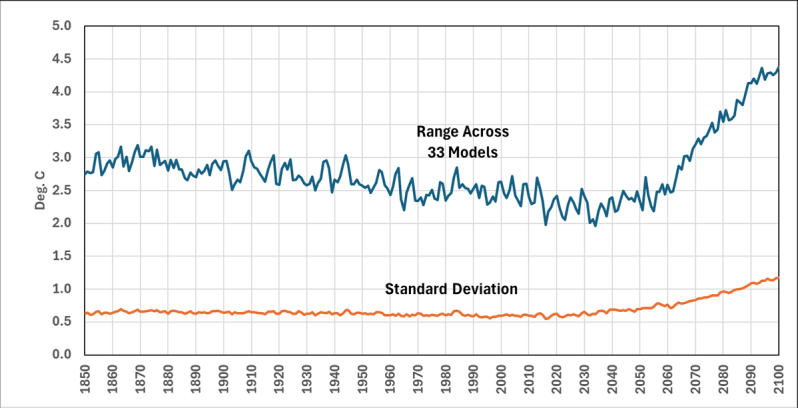
\includegraphics[width=.9\textwidth]{bilder/bilderKlima-0024.png}
  \captionof{figure}{CMIP6 Durchschnittliche Oberflächentemperaturspanne über 33 Modelle und Standardabweichung unter Verwendung des SSP5-85-Szenarios. Daten: KNMI Climate Explorer (\url{https://climexp.knmi.nl/start.cgi}).}
\end{minipage}

Jenseits der Fähigkeit der Modelle, Merkmale des heutigen Klimas zu reproduzieren, ist die kritische Frage für die Gesellschaft, wie gut sie Reaktionen auf subtile menschliche Einflüsse vorhersagen, wie Treibhausgasemissionen, Aerosol-Abkühlung und Landnutzungsänderungen. Der wichtigste Aspekt, den Modelle korrekt erfassen müssen, sind "Rückkopplungen". Diese treten auf, wenn Klimaänderungen entweder weitere Erwärmung verstärken oder unterdrücken. Im Allgemeinen verdoppelt oder verdreifacht der modellierte Nettoeffekt aller Rückkopplungen die direkte Erwärmungswirkung von CO$_2$.
\end{fullbox}

\section{Oberflächenerwärmung}
Ein einfacher Test der Gültigkeit eines Klimamodells ist seine Fähigkeit, historische Erwärmung als Reaktion auf bekannte vergangene Änderungen in Klimaantrieben wie Treibhausgasen zu reproduzieren. Abbildung 5.2 ist aus Scaffeta (2023) reproduziert, die die neueste Generation (CMIP6) von Klimamodellen in niedrige ECS ($1.5$ bis \SI{3.0}{\celsius}), mittlere ECS ($3.0$ bis \SI{4.5}{\celsius}) und hohe ECS ($4.5$ bis \SI{6.0}{\celsius}) gruppiert und ihre Post-1980 globalen Durchschnittstemperatur-Simulationsbereiche mit denen von drei Oberflächentemperaturaufzeichnungen und einem satelliten-basierten unteren Troposphärentemperatur-Datenprodukt vergleicht.
Die linke Spalte zeigt, dass die niedrig-ECS-Modelle die Post-1980 historische Erwärmungsaufzeichnung vernünftig gut verfolgen, aber die mittleren und rechten Spalten zeigen, dass die mittleren und hohen ECS-Modelle die Erwärmung auffällig über-vorhersagen.

\begin{figure}[H]
\begin{center}
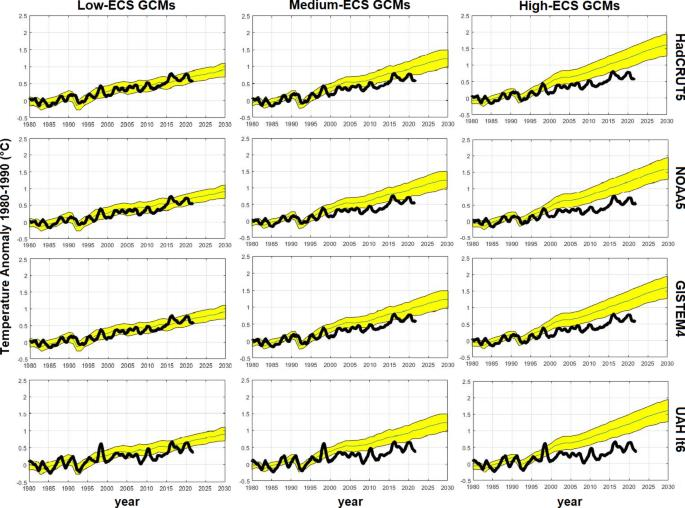
\includegraphics[width=1.0\textwidth]{bilder/bilderKlima-0026.jpg}\\[1cm]
\end{center}
\caption{Modell-Beobachtungs-Vergleiche für die Erwärmung der Erdoberfläche. Die Spalten entsprechen
Modellgruppen mit niedrigem ECS (13 Modelle), mittlerem ECS (11 Modelle) und hohem ECS (14 Modelle),
während die Zeilen den weit verbreiteten beobachteten Temperaturaufzeichnungen entsprechen, wobei die ersten drei
Oberflächendurchschnitte und die vierte den Durchschnitt der unteren Troposphäre zeigen. In jedem Feld bezeichnet der gelbe
Bereich den Mittelwert und die Spannweite (± eine Standardabweichung) der Klimamodellsimulationen für diese
Gruppe. Die dicke schwarze Linie zeigt die beobachtete jährliche Durchschnittstemperatur in der angegebenen Aufzeichnung.
Quelle: Scafetta (2023) Abb. 2.}
\end{figure}

Spencer (2024) hat auch eine nützliche Zusammenfassung der Modell-Beobachtungs-Diskrepanz bereitgestellt, indem er Trends in Oberflächentemperatur-Datenprodukten mit denen in einzelnen Klimamodellen verglich, wie in Abbildung 5.3 zusammengefasst; die meisten Klimamodelle zeigen erheblich mehr Erwärmung als die Beobachtungen seit 1979.

\begin{figure}[H]
\begin{center}
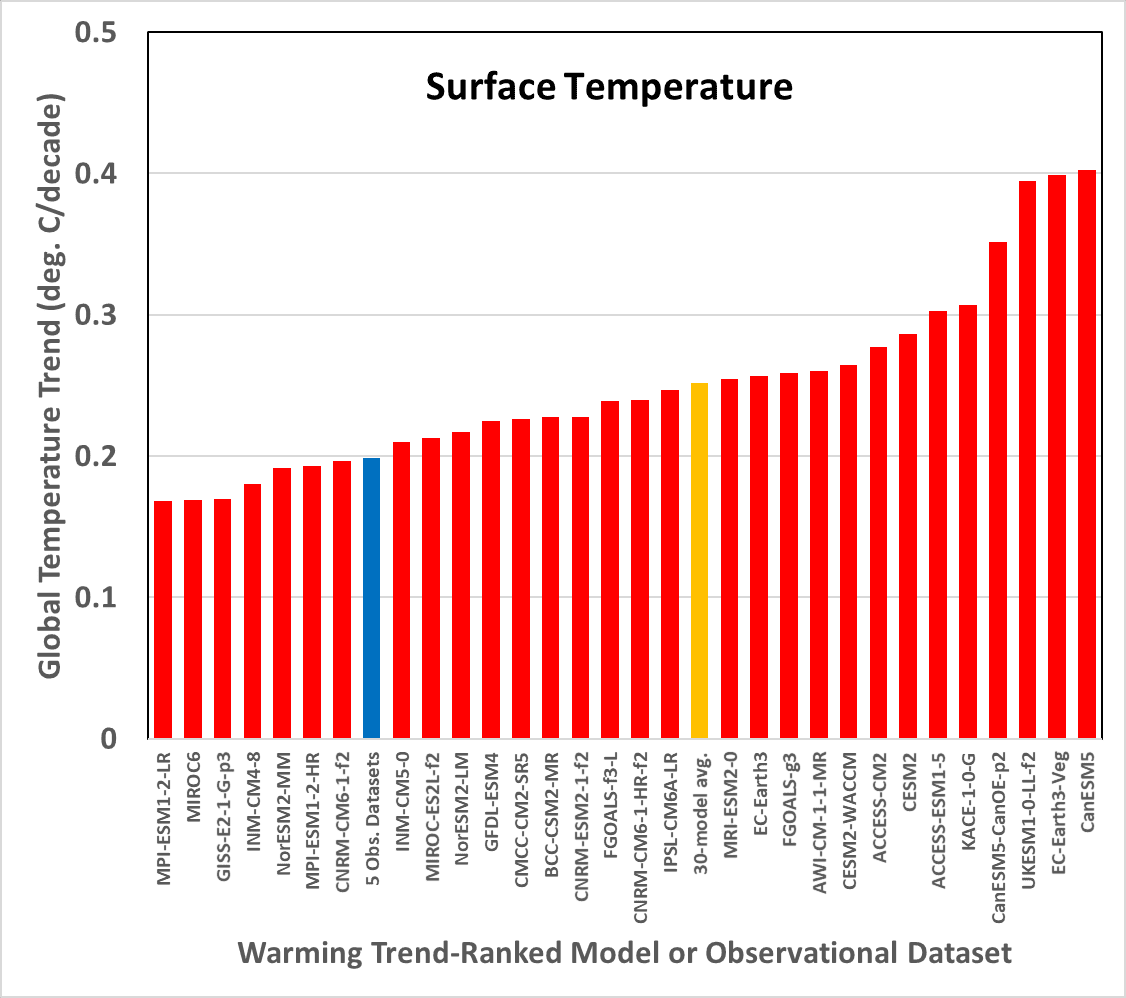
\includegraphics[width=1.0\textwidth]{bilder/bilderKlima-0027.png}\\[1cm]
\end{center}
\caption{Globale Trends der Oberflächenlufttemperatur (°C/Jahrzehnt), 1979–2024, aus verschiedenen CMIP6-Klimamodellen
(rot, Durchschnitt von 30 Modellen in orange); und der Durchschnitt von drei Thermometer-Datensätzen
(HadCRUT5, NOAA Global Temp und Berkeley 1 deg.) und zwei Reanalyse-Datensätzen (ERA5 und
NCEP/NCAR R1) in blau. Datenquelle: https://climexp.knmi.nl/start.cgi.}
\end{figure}

\section{Troposphärische Erwärmung}
Es ist seit langem bekannt, dass Klimamodelle im Durchschnitt die Erwärmung in der tropischen Troposphäre übertreiben. Diese Region ist ein wichtiger Test für Klimamodelle, da hier das Signal anthropogener Treibhauserwärmung zuerst und am stärksten auftritt. Verzerrungen in troposphärischen Trends zeigen Modellfehler in Wärmeübertragungsprozessen an, die sich auf Oberflächenerwärmungsverzerrungen übertragen.

Die Diskrepanz wurde als ernste Inkonsistenz im ersten U.S. Climate Change Science Program-Bericht (Karl et al. 2006) markiert und wurde in jedem IPCC-Bericht seitdem erwähnt, aber die Diskrepanz hat sich mit der Zeit verschlechtert, und die Verzerrung ist nun global. McKitrick und Christy (2020) verglichen troposphärische Erwärmungstrends in CMIP6-Klimamodellen mit beobachteten Trends von Satelliten, Wetterballons und Reanalysesystemen. Jedes Modell überschätzte den durchschnittlichen beobachteten Erwärmungstrend über 1979-2014 sowohl in unteren als auch mittleren Troposphärenschichten, sowohl global als auch in den Tropen. In den meisten einzelnen Modellen war die Verzerrung statistisch signifikant und im Durchschnitt über alle Modelle war sie hoch signifikant.

Abbildung 5.4 präsentiert die Vergleiche mit auf 2024 aktualisierten Daten (McKitrick und Christy 2025). Die jüngsten warmen Jahre bewegten den beobachteten Trend leicht nach oben und erweiterten die Trend-Konfidenzintervalle, aber das Gesamtmuster bleibt das gleiche: Modellverzerrung tendiert zu zu viel Erwärmung, in den meisten Fällen ist der Unterschied statistisch signifikant und im Durchschnitt ist die Verzerrung statistisch hoch signifikant. McKitrick und Christy (2020) zeigten auch, dass die Verzerrung in Modellen mit hoher ECS größer ist, aber selbst die Modelle mit niedrigerer durchschnittlicher ECS sagen zu viel Erwärmung vorher. Wenn zukünftige Klimamodelle globale troposphärische Erwärmung realistisch repräsentieren würden, wären sie wahrscheinlich weniger sensitiv als selbst die niedrig-ECS-Mitglieder des CMIP6-Ensembles.

\begin{figure}[H]
\begin{center}
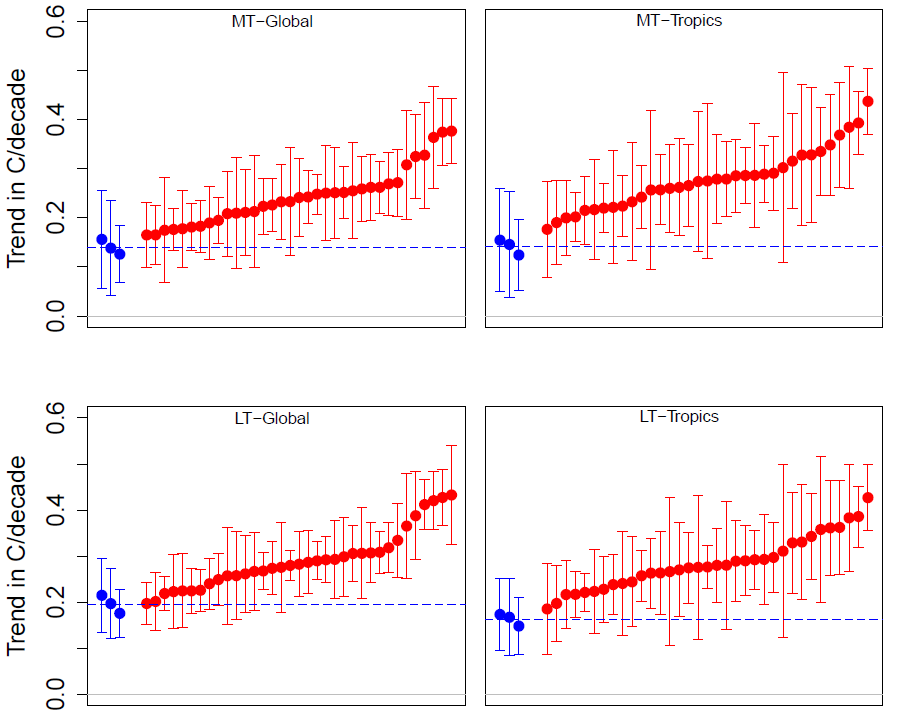
\includegraphics[width=1.0\textwidth]{bilder/bilderKlima-0028.png}\\[1cm]
\end{center}
\caption{Beobachtete gegenüber CMIP6-modellierten Erwärmungstrends (°C/Jahrzehnt 1979–2024) in der globalen
und tropischen unteren (LT) und mittleren Troposphäre (MT) unter Verwendung der Methodik von McKitrick und Christy
(2020) auf der Grundlage von Daten, die von 2014 bis 2024 aktualisiert wurden. Blaue Punkte: Erwärmungstrends mit 95-prozentigen Konfidenzintervallen
für 3 Datenprodukte (Radiosonden, Reanalyse und Satelliten). Blaue gestrichelte Linie: Durchschnittlicher Erwärmungstrend
für 3 beobachtete Reihen. Rote Punkte: Modellierte Erwärmungstrends mit 95-prozentigen Konfidenzintervallen
in 35 Modellen, angeordnet vom niedrigsten zum höchsten Wert.}
\end{figure}


Wie zuvor erwähnt, hat das IPCC die Modell-Beobachtungs-Diskrepanz lange anerkannt. Zum Beispiel bietet AR6 S. 443-444 dies zur tropischen Troposphäre (es behandelt nicht den globalen Vergleich):


\begin{quote}
Mehrere Studien seit AR5 haben weiterhin eine Inkonsistenz zwischen simulierten und beobachteten Temperaturtrends in der tropischen Troposphäre demonstriert, wobei Modelle mehr Erwärmung simulieren als Beobachtungen (Mitchell et al., 2013, 2020; Santer et al., 2017a, b; McKitrick und Christy, 2018; Po-Chedley et al., 2021)... Über den Zeitraum 1979–2014 sind Modelle konsistenter mit Beobachtungen in der unteren Troposphäre und am wenigsten konsistent in der oberen Troposphäre um 200 hPa, wo Verzerrungen \SI{0.1}{\celsius} pro Jahrzehnt überschreiten.
Mehrere Studien mit CMIP6-Modellen legen nahe, dass Unterschiede in der Klimasensitivität ein wichtiger Faktor sein könnten, der zur Diskrepanz zwischen simulierten und beobachteten troposphärischen Temperaturtrends beiträgt (McKitrick und Christy, 2020; Po-Chedley et al., 2021), obwohl es schwierig ist, den Einfluss von Klimasensitivität, Änderungen in Aerosolforcing und interner Variabilität bei der Beitragung zu troposphärischen Erwärmungsverzerrungen zu entschlüsseln (Po-Chedley et al., 2021). Eine andere Studie fand, dass das Fehlen einer hypothetischen negativen tropischen Wolkenrückkopplung die Hälfte der oberen Troposphären-Erwärmungsverzerrung in einem Modell erklären könnte (Mauritsen und Stevens, 2015).

... Zusammenfassend finden Studien weiterhin, dass CMIP5- und CMIP6-Modell\-simulationen mehr erwärmen als Beobachtungen in der tropischen mittleren und oberen Troposphäre über den Zeitraum 1979–2014 (Mitchell et al., 2013, 2020; Santer et al., 2017a, b; Suárez-Gutiérrez et al., 2017; McKitrick und Christy, 2018), und dass überschätzte Oberflächenerwärmung teilweise verantwortlich ist (Mitchell et al., 2013; Po-Chedley et al., 2021). ... Daher bewerten wir mit mittlerem Vertrauen, dass CMIP5- und CMIP6-Modelle weiterhin beobachtete Erwärmung in der oberen tropischen Troposphäre über den Zeitraum 1979–2014 um mindestens \SI{0.1}{\celsius} pro Jahrzehnt überschätzen.
\end{quote}

Bemerkenswert ist, dass trotz der Anhäufung von Belegen für überschüssige Modellerwärmung das IPCC nur mittleres Vertrauen in die Existenz einer Erwärmungsverzerrung zuordnet.

\section{Diskrepanz des vertikalen Temperaturprofils}
Eine weitere wichtige Modell-Beobachtungs-Diskrepanz ist die überschüssige Verstärkung mit der Höhe, die in Klimamodellen gefunden wird. Der Vergleich war in AR5 Kapitel 10, allerdings nur im Online-Supplement (Abbildung 10.SM.1) und nur in einer Abbildung, deren Formatierung den Punkt verdeckte. Abbildung 10.SM.1 wird weder im Haupt-IPCC-Bericht noch in irgendeiner Zusammenfassung referenziert, sodass Leser nicht davon gewusst hätten. Obwohl auf den ersten Blick nicht ersichtlich, zeigt sie, dass die Erwärmung von 1979-2010 in der unteren Troposphäre so gering ist, dass sie mit gar keinem THG-Forcing konsistent ist und inkonsistent mit den Modellläufen, die THG-Forcing haben. In Abbildung 5.6 adaptieren wir IPCC AR5 Abbildung 10.SM.1, um diesen kritischen Punkt herauszuarbeiten.

\begin{figure}[H]
\begin{center}
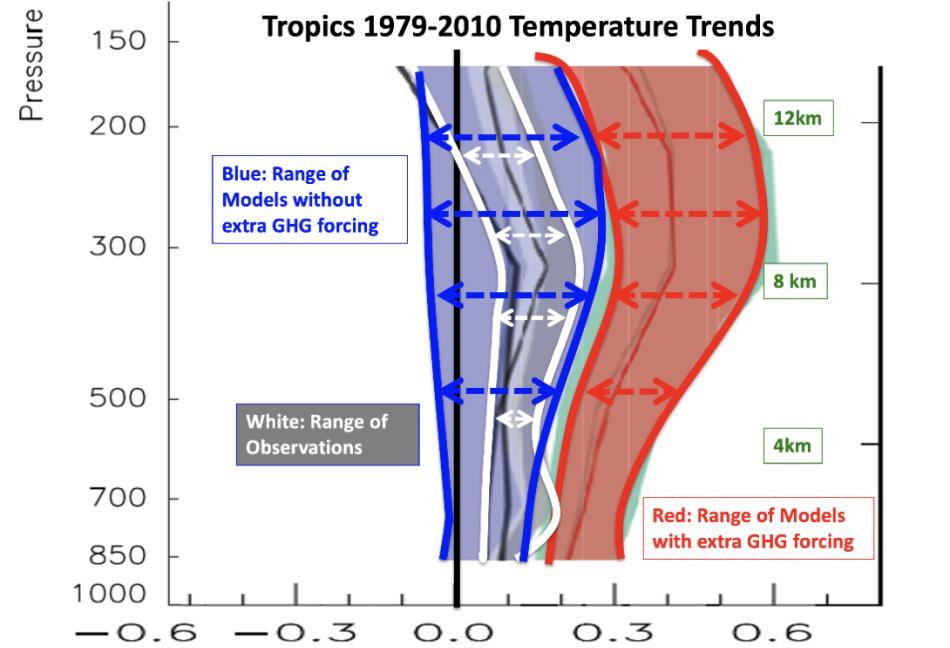
\includegraphics[width=1.0\textwidth]{bilder/bilderKlima-0029.jpg}\\[1cm]
\end{center}
\caption{Vertikales Erwärmungsmuster für die Tropen (\SI{20}{\degree}S bis \SI{20}{\degree}N). Horizontale Achse:
\si{\degree}/Jahrzehnt. Quelle: Kommentierte Version von IPCC AR5 Abbildung 10.SM.1}
\end{figure}

Abbildung 5.5 vergleicht Modell- und Beobachtungstemperaturtrends nach Höhe zwischen 20S und 20N (den Tropen). In dieser Region, wo die Modelle sagen, dass die Erwärmung am stärksten sein sollte, liegen die Beobachtungen (hier in weiß gezeigt) innerhalb des blauen \emph{Kein CO$_2$}-Bandes und völlig außerhalb der \emph{mit CO$_2$} roten Hülle. Das bedeutet, dass in der gesamten tropischen atmosphärischen Säule von der Oberfläche bis zur Basis der Stratosphäre beobachtete Erwärmungstrends so klein sind, dass sie mit der Ausgabe von Modellen konsistent sind, die kein anthropogenes CO$_2$ haben, und inkonsistent mit der gesamten Hülle von Erwärmungstrends, die von Modellen generiert werden, die mit erhöhtem CO$_2$ forciert werden.

Ein ähnlicher Vergleich wird in Christy und McNider (2017) gezeigt, eine aktualisierte Version davon (abdeckend 1979-2024) ist als Abbildung 5.6 reproduziert. Modellierte Temperaturtrends überschreiten Beobachtungen von der Oberfläche bis zur Spitze der Troposphäre, mit beobachteten Trends unterhalb des gesamten Modellbereichs auf den meisten Druckniveaus. Auch in Abbildung 5.6 gezeigt ist der tropische troposphärische Temperatur (TTT) Durchschnitt von drei Satellitendatenprodukten (NOAA, UAH und RSS) verglichen mit dem gleichen Schichtdurchschnitt von Klimamodellen für 1979-2024. Wieder liegen die beobachteten Trends unterhalb des gesamten Modellbereichs.

Die weite Spannweite der Entscheidungen, die von Modellierern getroffen werden, um die physikalischen Prozesse in den Modellen zu charakterisieren (siehe Kasten: Klimamodellierung in Abschnitt 5.1 oben), wird durch die große Streuung der Trends in der mittleren Troposphäre gesehen, ±40 Prozent um den Median (Abbildung 5.6). Dies illustriert lebhaft die Unsicherheiten in Versuchen, ein komplexes System zu modellieren (parametrisieren), das Turbulenz, feuchte Thermodynamik und Energieflüsse über den vollen Bereich der Zeit- und Raumskalen der tropischen Atmosphäre umfasst.

\begin{figure}[H]
\begin{center}
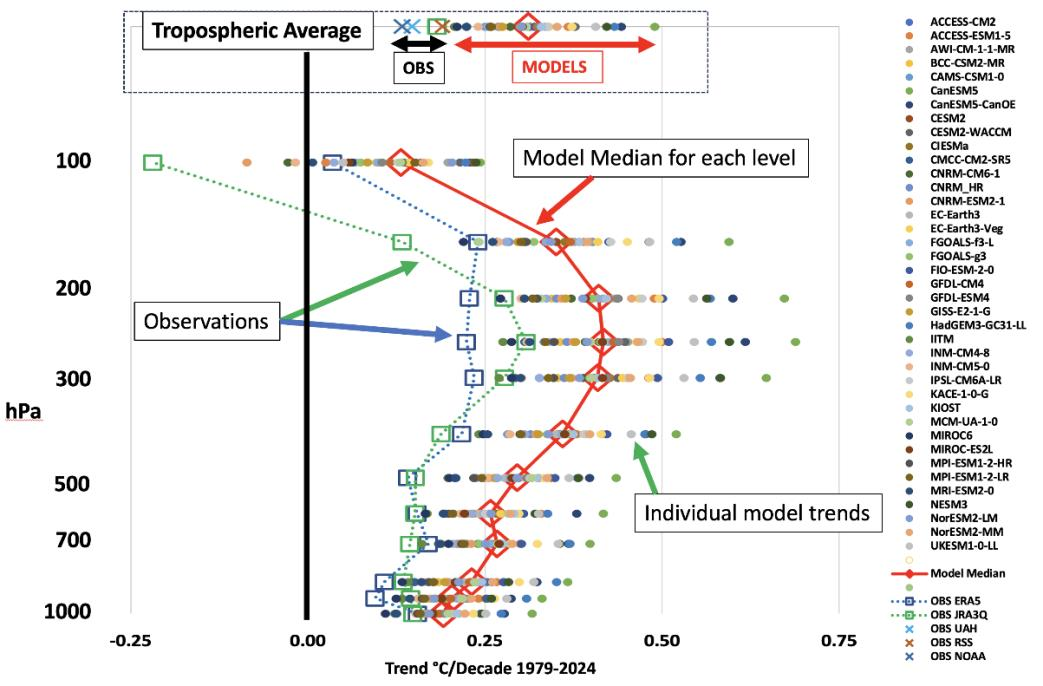
\includegraphics[width=1.0\textwidth]{bilder/bilderKlima-0030.jpg}\\[1cm]
\end{center}
\caption{Modellierte versus beobachtete Erwärmung, tropische Troposphäre. Quelle: aktualisiert
nach Christy und McNider (2017) einschließlich Daten bis 2024 und CMIP6-Modellausgaben.
Rote Linie: Modelldurchschnitt. Grüne und blaue Linien: Beobachtungsreihen (Reanalyse).}
\end{figure}

Diese Diskrepanz war die Quelle viel Kontroverse, wobei einige argumentierten, dass, selbst wenn es sehr wenig beobachtete Erwärmung in der Höhe in den Tropen gibt, ein "Hotspot" trotzdem existiert in dem Sinne, dass die Erwärmung in der Höhe größer ist als an der Oberfläche (Santer et al. 2008). Aber es gibt gute Belege, dass Modelle auch die Verstärkungsrate übertreiben. Klotzbach et al. (2009) zeigten, dass Modelle größere Verstärkung mit der Höhe projizieren, als beobachtet wird. Dieses Ergebnis wurde anschließend durch detaillierte Zeitreihenanalyse bestätigt (Vogelsang und Nawaz 2016), die fand, dass der Modell-Beobachtungs-Unterschied statistisch signifikant ist.
Das Temperaturprofil der Atmosphäre ist ein Fall, wo Modelle nicht nur unsicher sind, sondern auch eine gemeinsame Erwärmungsverzerrung relativ zu Beobachtungen zeigen. Das legt nahe, dass sie bestimmte fundamentale Rückkopplungsprozesse falsch darstellen.

Das IPCC AR6 bewertete dieses Problem nicht.


\section{Stratosphärische Abkühlung}
Ein wichtiges Element des erwarteten allgemeinen "Fingerabdrucks" des anthropogenen Klimawandels ist gleichzeitige Erwärmung der Troposphäre und Abkühlung der Stratosphäre. Das letztere Merkmal wird auch durch Ozonabbau und -erholung beeinflusst. AR6 anerkannte, dass Abkühlung beobachtet worden war, aber nur bis zum Jahr 2000. Die Stratosphäre hat seitdem eine gewisse Erwärmung gezeigt, entgegen Modellprojektionen.

AR6 WG1 Kap 2 S. 327-9 stellt fest:
\begin{quote}
Temperaturen, die über die gesamte untere Stratosphäre (etwa 10–25 km) gemittelt wurden, haben über 1980–2019 in allen Datenprodukten abgenommen, wobei der Großteil der Abnahme vor 2000 lag. Die Abnahme besteht auch, wenn der Einfluss der El Chichon (1982) und Pinatubo (1991) Vulkanausbrüche auf den Trend, von dem Steiner et al. (2020a) fanden, dass er den 1979–2018 Abkühlungstrend um \SI{0.06}{\celsius} pro Jahrzehnt erhöht hat, entfernt wird. Die meisten Datensätze zeigen keine signifikanten oder nur marginal signifikante Trends über 2000–2019, und die Ergebnisse von Philipona et al. (2018) zeigen schwache Zunahmen über 2000–2015 in der allertiefsten Stratosphäre, die von Radiosonden beprobt wird....

Es ist praktisch sicher, dass sich die untere Stratosphäre seit der Mitte des 20. Jahrhunderts abgekühlt hat. Jedoch zeigen die meisten Datensätze, dass sich untere stratosphärische Temperaturen seit Mitte der 1990er Jahre stabilisiert haben ohne signifikante Änderung über die letzten 20 Jahre. Es ist wahrscheinlich, dass sich mittlere und obere stratosphärische Temperaturen seit 1980 verringert haben, aber es gibt geringes Vertrauen in das Ausmaß.
\end{quote}

Die zitierte Quelle, Philipona et al. (2018), in einem Artikel mit dem Titel "Radiosonden zeigen, dass nach Jahrzehnten der Abkühlung sich die untere Stratosphäre jetzt erwärmt", stellte fest:
\begin{quote}
Als Reaktion auf fortgesetzte Treibhausgaserhöhungen und stratosphärischen Ozonabbau projizieren Klimamodelle fortgesetzte troposphärische Erwärmung und stratosphärische Abkühlung über die kommenden Jahrzehnte. Globale durchschnittliche Satellitenbeobachtungen unterer stratosphärischer Temperaturen zeigen keine signifikanten Trends seit der Jahrhundertwende. Im Gegensatz dazu zeigt eine Analyse vertikal aufgelöster Radiosondenmessungen von 60 Stationen eine Zunahme der unteren stratosphärischen Temperatur seit der Jahrhundertwende in Höhen zwischen 15 und 30 km und über den meisten Kontinenten. Trendschätzungen sind etwas empfindlich gegenüber Homogenitätsbewertungswahlmöglichkeiten, aber alle untersuchten Radiosondendatensätze legen eine Änderung von Abkühlung im späten zwanzigsten Jahrhundert zu Erwärmung im frühen 21. Jahrhundert in der unteren Stratosphäre nahe.
\end{quote}

Santer et al. (2023) verwenden aktualisierte Daten, um zu zeigen, dass ein Abkühlungstrend in der unteren Stratosphäre nicht wieder aufgetaucht ist.

Eine Kombination aus troposphärischer Erwärmung und stratosphärischer Abkühlung ist ein häufig zitierter "Fingerabdruck" des anthropogenen Klimawandels. Stratosphärische Erwärmung seit 2000 fällt mit fortgesetzter Oberflächen- und troposphärischer Erwärmung zusammen, ein Muster, das in Klimamodellsimulationen nicht gefunden wird und anscheinend nicht konsistent mit dem anthropogenen Fingerabdruck ist.

\section{Diskrepanz der Schneebedeckung}
Daten, die vom Rutgers University Snow Lab zusammengestellt wurden, zeigen, dass die Winterschneebedeckung der Nordhemisphäre nicht abnimmt (Abbildung 5.7); wenn überhaupt, zeigt sie einen zunehmenden Trend.

\begin{figure}[H]
\begin{center}
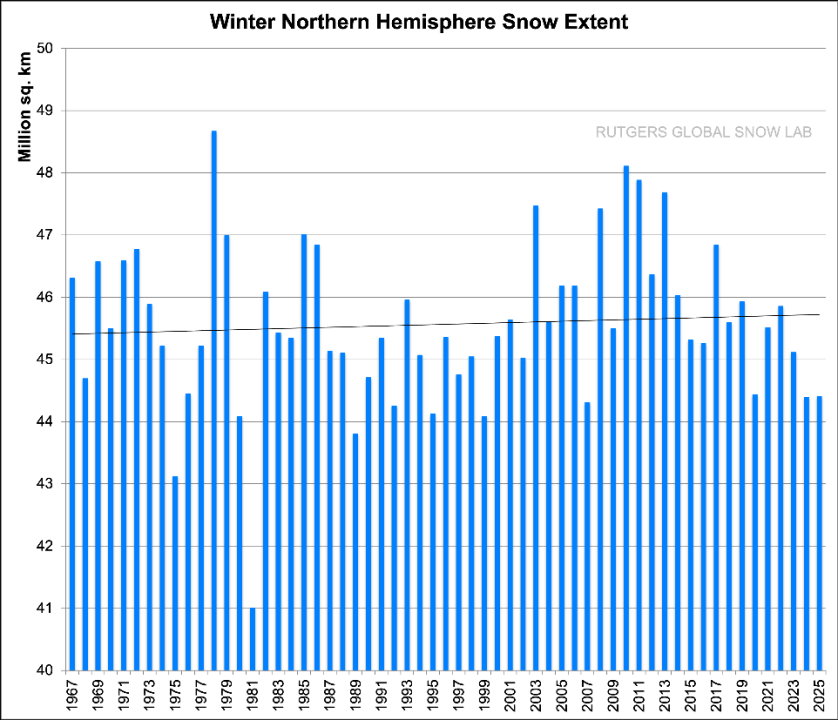
\includegraphics[width=1.0\textwidth]{bilder/bilderKlima-0031.png}\\[1cm]
\end{center}
\caption{Schneebedeckung im Winter auf der Nordhalbkugel.
Quelle: \url{https://climate.rutgers.edu/snowcover/chart_seasonal.php?ui_set=nhland&ui_season=1}
(abgerufen am 27. Mai 2025)}
\end{figure}

Dennoch projizieren Modelle abnehmende Schneebedeckung der Nordhemisphäre in einem sich erwärmenden Klima, wie von Connolly et al. (2019) beschrieben.
\begin{quote}
Es wurde gefunden, dass die Klimamodelle die beobachteten Trends [in der Schneebedeckung der Nordhemisphäre] schlecht erklären. Während die Modelle nahelegen, dass Schneebedeckung für alle vier Jahreszeiten stetig hätte abnehmen sollen, zeigten nur Frühling und Sommer eine langfristige Abnahme, und das Muster der beobachteten Abnahmen für diese Jahreszeiten war ziemlich unterschiedlich von den modellierten Vorhersagen. Darüber hinaus legen die beobachteten Trends für Herbst und Winter eine langfristige Zunahme nahe, obwohl diese Trends nicht statistisch signifikant waren.
\end{quote}

AR6 beschränkt seine Diskussion der sich ändernden Schneebedeckungsausdehnung (SCE) der Nordhemisphäre weitgehend auf die Frühlingssaison, für die Modelle und Beobachtungen in einem Abwärtstrend übereinstimmen. Bezüglich Winteränderungen bemerkt es wie folgt (AR6 WGI Kap. 2 S. 344):
\begin{quote}
Die Bewertung von SCE-Trends in der NH seit 1978 zeigt, dass für den Oktober bis Februar Zeitraum erhebliche Unsicherheit in Trends besteht, wobei das Vorzeichen vom Beobachtungsprodukt abhängt. Analyse mit dem NOAA Climate Data Record zeigt eine Zunahme in Oktober bis Februar SCE (Hernández-Henríquez et al., 2015; Kunkel et al., 2016), während Analysen basierend auf satellitengetragenen optischen Sensoren (Hori et al., 2017) oder Multi-Beobachtungsprodukten (Mudryk et al., 2020) einen negativen Trend für alle Jahreszeiten zeigen.
\end{quote}

AR6 WGI Kapitel 9 (S. 1284) weist darauf hin, dass der NOAA Climate Data Record, der erhöhte Herbst- und Winter-SCE zeigt, inkonsistent mit landbasierten Beobachtungen und modellbasierten Datensätzen ist. Es bemerkt, dass die Verwendung optischer Satellitenbilder zur Ableitung von SCE im Winter aufgrund von Wolkenbedeckung und verringerter Sonnenbeleuchtung in Wintermonaten herausfordernd ist. Mit Fokus auf die Pazifikküstenstaaten (CA, OR und WA) stellt kaltsaisonaler Bergschneefall, der im Frühling und Sommer schmilzt, einen erheblichen Teil der warmsaisonalen Wasserressourcen bereit.
Eine umfassende Rekonstruktion des Schneefalls für die Hauptquellregionen (Cascade- und Sierra-Nevada-Berge) zeigt keine signifikanten Trends in jährlichen Gesamtsummen seit dem späten 19. Jahrhundert (Christy 2022).

Zusammenfassend zeigt die aktuelle Rutgers SCE-Datenbank eine Diskrepanz zwischen Modellen und Beobachtungen an. Weitere Arbeit zur Versöhnung widersprüchlicher Trends in Beobachtungsdatensätzen ist erforderlich.

\section{Hemisphärische Symmetrie der planetaren Albedo}
Die planetare Albedo ist der Anteil der einkommenden Sonnenstrahlung, der von der Erde zurück in den Weltraum reflektiert wird. Sie ist ein wichtiges Element der strahlenden Energiebilanz und beeinflusst, ob sich der Planet über die Zeit erwärmen oder abkühlen wird. Die planetare Albedo wird typischerweise auf etwa 0,30 geschätzt; Variationen im Maßstab von 0,01 entsprechen Änderungen im Solarforcing von etwa \SI{3}{\watt\per\square\meter}, einem Betrag, der größer ist als das aktuelle anthropogene Forcing. Es wurde seit langem bemerkt, dass Modelle untereinander und mit Beobachtungen über den Wert der globalen planetaren Albedo uneinig sind (Stephens et al. 2015).

Eine faszinierende Eigenschaft der Erdalbedo ist, dass im Durchschnitt die Nordhemisphäre (NH) und Südhemisphäre (SH) nahezu die gleiche Albedo hatten, zumindest während der fünfzigjährigen Satellitenaufzeichnung (Stephens et al., 2015). Diese Symmetrie ist überraschend, weil die SH viel mehr Ozean als Land hat. Da Ozean weniger reflektierend ist als Land, sollte die NH höhere Albedo haben. Wolken (die hochreflektierend sind) sind in der NH häufiger und kompensieren so die Oberflächenalbedo-Ungleichgewichte der zwei Hemisphären. Datseris und Stephens (2021) zeigen, dass diese Wolkenkompensation von den außertropischen Sturmbahnen der SH kommt, die wolkiger sind als die der NH. Während der Mechanismus für diese hemisphärische Symmetrie unklar ist, operiert er wahrscheinlich auf großen zeitlichen und räumlichen Skalen.

Die hemisphärische Symmetrie der Albedo ist eine einfache grobe Metrik für Klimamodelle. Rugenstein und Hakuba (2023) definierten diese Metrik als den Unterschied zwischen den jährlichen Mittelalbedos von NH und SH, ausgedrückt als \si{\watt\per\square\meter} des reflektierten Sonnenlichts, und stellten sie für die CMIP6-Klimamodelle zusammen, wie in Abbildung 5.8 gezeigt. Die meisten CMIP6-Modelle reproduzieren die kleine beobachtete Asymmetrie (etwa \SI{0.1}{\watt\per\square\meter}) nicht und sind sich sogar uneinig darüber, welche Hemisphäre reflektierender ist. Darüber hinaus reicht das Ausmaß der Asymmetrie in einigen Modellen bis zu \SI{5}{\watt\per\square\meter}, zweimal so groß wie das aktuelle anthropogene Forcing (etwa \SI{2.7}{\watt\per\square\meter}).

Die Bedeutung unphysikalischer Albedo-Asymmetrien in den Klimamodellen ist noch nicht vollständig bekannt. Jedoch legen andere Modellstudien nahe, dass interhemisphärische Änderungen in der Albedo polwärtige Wärmeflüsse, meridionale Temperaturgradienten, Sturmhäufigkeit und Unterschiede in hemisphärischer ozeanischer Wärmespeicherung verändern können. Die Diskrepanz zwischen Modellen und Beobachtungen wirft weitere Fragen bezüglich Wolken-Rückkopplungsprozessen auf und verringert so allgemeiner das Vertrauen in Modellprojektionen des zukünftigen Klimas.
\begin{figure}[H]
\begin{center}
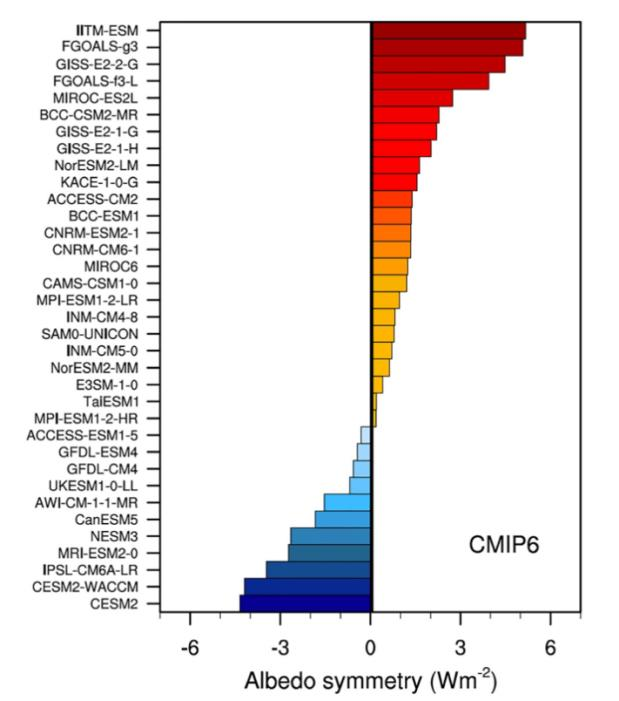
\includegraphics[width=1.0\textwidth]{bilder/bilderKlima-0033.jpg}\\[1cm]
\end{center}
\caption{Unterschiede in der durchschnittlichen Reflektivität (Albedo) über 20 Jahre zwischen der nördlichen und
südlichen Hemisphäre für CMIP6-Modelle, die in der jüngsten IPCC-Bewertung verwendet wurden (farbige Balken).
Der sehr geringe beobachtete Unterschied wird durch die vertikale schwarze Linie angezeigt. Aus Rugenstein und
Hakuba (2023).}
\end{figure}

\section{U.S. Corn Belt}
Eine der größten Diskrepanzen zwischen Modellen und Beobachtungen liegt im U.S. Corn Belt, einer Region von besonderer Bedeutung für die globale Nahrungsmittelproduktion. Abbildung 5.9 zeigt die Erwärmungstrends für die Sommerzeit (Juni, Juli, August) für den 12-Staaten Corn Belt (IN, IA, IL, ND, SD, MO, MN, WI, MI, OH, KS, NE) während 1973-2022. Alle 36 Klimamodelle (rot) erwärmen sich viel zu schnell verglichen mit Beobachtungen (blau).

\begin{figure}[H]
\begin{center}
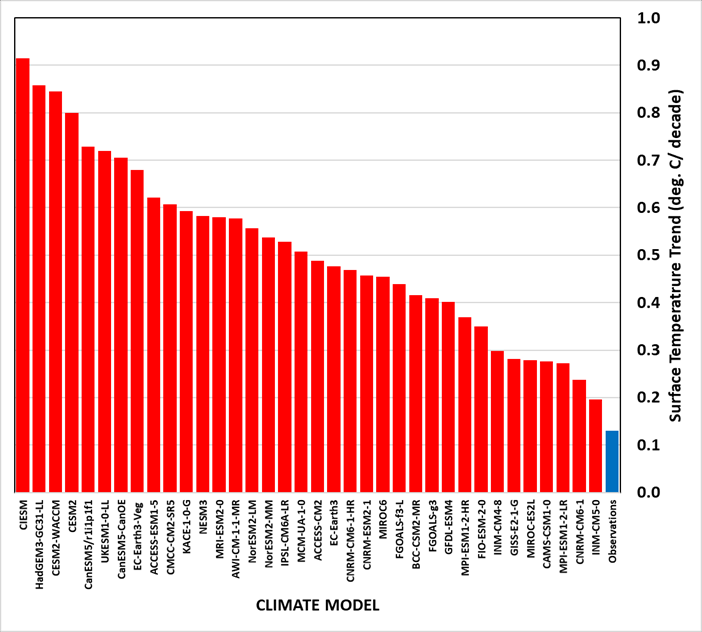
\includegraphics[width=1.0\textwidth]{bilder/bilderKlima-0034.png}\\[1cm]
\end{center}
\caption{Modellierte versus beobachtete Erwärmungstrends im US-amerikanischen Maisgürtel, 1973–2022.}
\end{figure}

Wie in Kapitel 9 diskutiert, sind die erwarteten negativen Effekte steigender Temperaturen auf U.S. Maiserträge nicht eingetreten, im Gegensatz zu weit publizierten Studien, die proklamieren, dass theoretische zukünftige Auswirkungen bereits erfahren werden (z.B., Seager et al., 2018).

Das IPCC erkennt Begrenzungen in der Genauigkeit regionaler Klimamodell-Ausgaben an. Dieses Beispiel zeigt, dass Nutzer Modellprojektionen sorgfältig von Fall zu Fall bewerten müssen, da lokale Verzerrungen möglicherweise ausreichend groß sind, dass die Modelle einfach nicht für den Zweck geeignet sind. Wie kürzlich von zwei Führern der Modellierungsgemeinschaft bemerkt wurde (Hervorhebung hinzugefügt):
\begin{quote}
... für viele Schlüsselanwendungen, die regionale Klimamodell-Ausgaben erfordern oder für die Bewertung großmaßstäblicher Änderungen aus kleinmaßstäblichen Prozessen, glauben wir, dass die aktuelle Generation von Modellen nicht für den Zweck geeignet ist. (Palmer und Stevens 2019)
\end{quote}

Zusammenfassend:
\begin{itemize}
\item Klimamodelle zeigen Erwärmungsverzerrungen in vielen Aspekten ihrer Reproduktion der vergangenen wenigen Jahrzehnte.
\item  Sie produzieren zu viel Erwärmung an der Oberfläche (außer in den Modellen mit niedrigster ECS), zu viel Erwärmung in der unteren und mittleren Troposphäre und zu viel Verstärkung der Erwärmung in der Höhe.
\item  Sie produzieren auch zu viel stratosphärische Abkühlung, zu viel Schneeverlust und zu viel Erwärmung im U.S. Corn Belt.
\item  Der hemisphärische Albedo-Unterschied in einzelnen Klimamodellen reicht weit in Vorzeichen und Größenordnung verglichen mit Beobachtungen. Der Bereich in \si{\watt\per\square\meter} ist dreimal größer als das direkte anthropogene Forcing von CO$_2$.
\item  Das IPCC hat einige dieser Probleme anerkannt, aber nicht alle.
\end{itemize}

\vfill
\noindent\textbf{Literaturverzeichnis:}

\begingroup
\parindent=0pt
\everypar{\hangindent=2em\hangafter=1\relax}

Christy, J. R., R. T. McNider (2017). Satellite bulk tropospheric temperatures as a metric for climate
sensitivity. Asia-Pacific Journal of Atmospheric Sciences 53, 511-518.
https://doi.org/10.1007/s13143-017-0070-z

Christy, J. R. (2022). Time series construction of Oregon and Washington snowfall since 1890 and an
update of California snowfall through 2020. Journal of Hydrometeorology 23, 1845-1860.
https://doi.org/10.1175/JHM-D-21-0178.1

Connolly, R., M. Connolly, W. Soon, et al. (2019). Northern Hemisphere snow-cover trends (1967–
2018): A comparison between climate models and observations. Geosciences 9, 135.
https://doi.org/10.3390/geosciences9030135

Datseris, G., B. Stevens (2021). Earth’s albedo and its symmetry. AGU Advances 2,
e2021AV000440. https://doi.org/10.1029/2021AV000440

Karl, T.R., S. J. Hassol, C. D. Miller, W. L. Murray, eds. (2006). Temperature Trends in the Lower
Atmosphere: Steps for Understanding and Reconciling Differences. U.S. Climate Change Science
Program/Subcommittee on Global Change Research.
\url{https://digital.library.unt.edu/ark:/67531/metadc12017/m2/1/high_res_d/sap1-1-final-all.pdf}

Klotzbach, P.J., R. A. Pielke, Sr., R. A. Pielke, Jr., J. R. Christy, R. T. McNider (2009). An alternative
explanation for differential temperature trends at the surface and in the lower troposphere.
Journal of Geophysical Research — Atmospheres 114(D21).
\url{https://doi.org/10.1029/2009JD011841}

McKitrick, R. and J. R. Christy (2020). Pervasive warming bias in CMIP6 tropospheric layers. Earth and
Space Science 7. https://doi.org/10.1029/2020EA001281

McKitrick, R., and J.R. Christy (2025), “Data and Code for DoE Report 2025”, Mendeley Data, V1, doi:
10.17632/8n9ks93vn7.1

Palmer, T., and B. Stevens (2019). The scientific challenge of understanding and estimating climate
change. Proceedings of the National Academy of Sciences 116(49), 24390–24395.
https://doi.org/10.1073/pnas.1906691116

Philipona, R., C. Mears, M. Fujiwara, et al. (2018). Radiosondes show that after decades of cooling, the
lower stratosphere is now warming. Journal of Geophysical Research—Atmospheres 123.
https://doi.org/10.1029/2018JD028901

Rugenstein, M., and M. Hakuba (2023). Connecting hemispheric asymmetries of planetary albedo and
surface temperature. Geophysical Research Letters 50, e2022GL101802.
https://doi.org/10.1029/2022GL101802

Santer B D, P.W. Thorne, L Haimberger et al. (2008) Consistency of modelled and observed temperature
trends in the tropical troposphere International Journal of Climatology 28 1703–22
https://rmets.onlinelibrary.wiley.com/doi/abs/10.1002/joc.1756


Santer, B.D. S. Po-Chedley, L. Zhao, C et al. (2023) Exceptional stratospheric contribution to human
fingerprints on atmospheric temperature, Proceedings of the National Academy of Sciences U.S.A. 120
(20) e2300758120, https://doi.org/10.1073/pnas.2300758120.

Scaffeta, N (2023) CMIP6 GCM ensemble members versus global surface temperatures. Climate Dynamics
60, 3091–3120 (2023). https://doi.org/10.1007/s00382-022-06493-w

Seager, R., J. Feldman, N. Lis, et al. (2017). Whither the 100th meridian? The once and future physical
and human geography of America’s arid–humid divide. Part II: The meridian moves east. Earth
Interactions 22. https://doi.org/10.1175/EI-D-17-0012.1

Spencer, R. W. (2024). Global warming: Observations vs. climate models. Environment Backgrounder,
The Heritage Foundation.
https://www.heritage.org/environment/report/global-warming-observations-vs-climate-models

Stephens, G. L., D. O'Brien, P.J. Webster et al. (2015). The albedo of Earth. Reviews of Geophysics.
https://doi.org/10.1002/2014RG000449

Vogelsang, T. and N. Nawaz (2016). Estimation and inference of linear trend slope ratios with an
application to global temperature data: Journal of Time Series Analysis 38.
https://doi.org/10.1111/jtsa.12209
\endgroup

\cleardoublepage
\FigureNumbersBySection
\chapter{Extrem Wetter}
\paragraph{Kapitelzusammenfassung}
\begin{quote}
Die meisten Arten von Extremwetter zeigen keine statistisch signifikanten langfristigen Trends über die verfügbare historische Aufzeichnung. Während es eine Zunahme heißer Tage in den USA seit den 1950er Jahren gegeben hat, ein Punkt, der von AR6 betont wird, sind die Zahlen immer noch niedrig relativ zu den 1920er und 1930er Jahren. Extreme konvektive Stürme, Hurrikane, Tornados, Überschwemmungen und Dürren zeigen beträchtliche natürliche Variabilität, aber langfristige Zunahmen werden nicht erkannt.
Einige Zunahmen in extremen Niederschlagsereignissen können in einigen Regionen über kurze Intervalle erkannt werden, aber die Trends bestehen nicht über lange Zeiträume und auf regionaler Ebene fort. Waldbrände sind in den USA nicht häufiger als sie in den 1980er Jahren waren. Die verbrannte Fläche nahm von den 1960er Jahren bis zu den frühen 2000er Jahren zu, sie ist jedoch niedrig verglichen mit dem geschätzten natürlichen Grundniveau. Die US-Waldbrandaktivität wird stark von Forstwirtschaftspraktiken beeinflusst.
\end{quote}

\section{Einleitung}
Wetterextreme mit hohem Einfluss, die gewöhnlich mit Temperatur, Niederschlag und/oder starkem Wind zusammenhängen, können Infrastruktur stören und daher die menschliche Gesundheit und das Wohlbefinden gefährden. Die Frage ist nicht, ob Extreme auftreten. Vielmehr ist es, ob es langfristige (dekadische) Änderungen in der Häufigkeit oder dem Charakter von Extremen gibt ("Detektion"), sowie das Ausmaß, in dem solche Änderungen und die damit verbundenen Änderungen in Gefahren durch anthropogene Emissionen von Treibhausgasen verursacht werden ("Attribution"; z.B., AR6 Seneviratne et al. 2021).

Prozessbasiertes Verständnis und einfache thermodynamische Argumente sind herangezogen worden, um zu behaupten, dass Erwärmung Extremwetterereignisse verschlechtert. Es ist jedoch naiv anzunehmen, dass jedes jüngste Extremereignis durch menschliche Einflüsse auf das Klima verursacht wird. Klima handelt von den statistischen Eigenschaften des Wetters über Jahrzehnte, nicht von einzelnen Ereignissen. Weiterhin gibt es nur etwa 130 Jahre zuverlässiger Beobachtungsaufzeichnungen, die statistisch analysiert werden können. Dieses kurze Intervall beginnt nicht einmal, alle Extremereignisse zu enthalten, die das Klimasystem von allein erzeugen kann. Über geologische Zeit hat das Klimasystem eine (im Wesentlichen) unendliche Vielfalt von Wettermustern und Extremen erzeugt, die Menschen nie beobachtet haben und die daher in den Datenbanken fehlen, die zur Bestimmung extremer Statistiken verwendet werden [siehe Gefahren kurzer Datenaufzeichnungen unten]. Aus diesem Grund erfordert die Attribution eines Extremereignisses, das in der Aufzeichnung beispiellos ist, Annahmen über das Ausmaß natürlicher Variationen.

Dieses Kapitel befasst sich mit der Detektion von Trends im Extremwetter, während Kapitel 8 kausale Attribution betrachtet, mit Abschnitt 8.4, der sich spezifisch mit Extremwetter befasst. Wenn kein Trend erkannt wird, dann gibt es klar keine Basis für Attribution. Aber selbst wo ein Trend beobachtet wird, folgt Attribution zu menschlich verursachter Erwärmung nicht notwendigerweise.

Das ist besonders wahr für Niederschlagsereignisse. Die hydrologische Literatur hat seit langem das Vorhandensein langer, langsamer und unregelmäßiger Oszillationen in Niederschlagsdaten bemerkt (Hurst 1951, Cohn und Lins 2005, Markonis und Koutsoyiannis 2016). Die Charakteristika dieser natürlichen Muster erfordern lange Aufzeichnungen, um Variabilität genau zu schätzen. Analyse von Aufzeichnungen, die kurz sind relativ zur Skala natürlicher Variabilität, wird dazu tendieren, Trends falsch darzustellen, daher die Signifikanz scheinbarer Trends zu übertreiben und die Wahrscheinlichkeit von Extremereignissen zu unterschätzen (Cohn und Lins 2005).

\begin{figure}[H]
\begin{center}
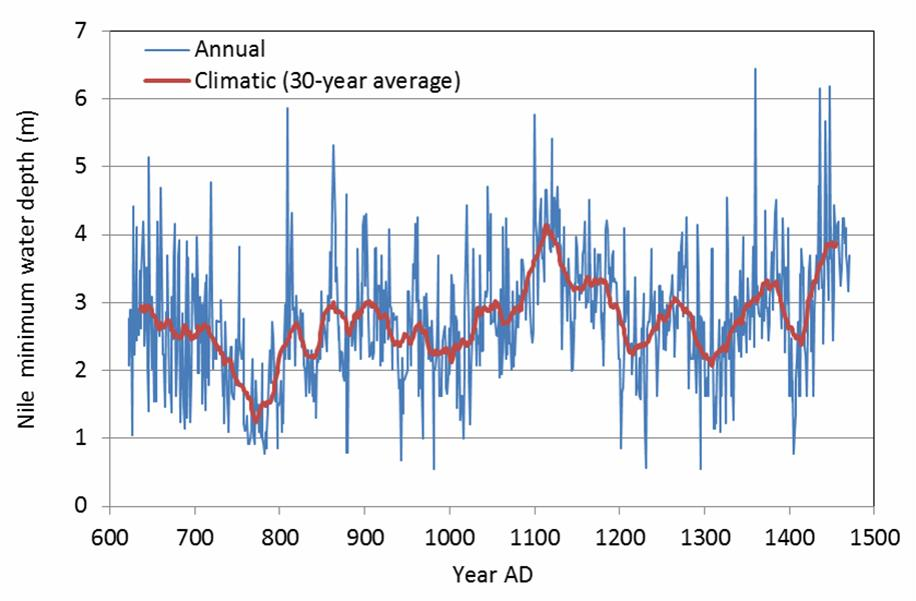
\includegraphics[width=1.0\textwidth]{bilder/bilderKlima-0036.jpg}\\[1cm]
\end{center}
\caption{Die jährliche Mindesttiefe des Nils in der Nähe von Kairo über einen Zeitraum von mehr als 650
Jahren von 622 bis 1284 n. Chr. Die in Metern gemessenen Daten zeigen ein charakteristisches Muster
von jährlichen Schwankungen um längerfristige Trends herum. Daten von Koutsoyiannis (2013)}
\end{figure}

Ein gutes Beispiel dafür ist die acht Jahrhunderte lange Aufzeichnung der jährlichen Mindesthöhe des Nils, die auf der Roda-Insel in Kairo beobachtet wurde, gezeigt in Abbildung 6.1.1. Der Nil wird von Niederschlag über ein 4 Millionen Quadratmeilen großes Einzugsgebiet gespeist, ein Gebiet gleich etwa einem Drittel von CONUS. Da menschliche Einflüsse auf das globale Klima lange vor dem 20. Jahrhundert vernachlässigbar waren, ist die jahrhundertliche Variabilität des dreißigjährigen Durchschnitts völlig natürlich; Ägypter des siebten und achten Jahrhunderts wären falsch gelegen anzunehmen, dass die sich verschlechternde Dürre während dieser Zeit das \emph{neue Normal} war.

Mit diesen Vorbehalten im Hinterkopf untersuchen wir die Belege für Änderungen in ausgewählten Wetter- und Klimaextremen. Ein wiederkehrendes Thema ist die weite Kluft zwischen öffentlichen Wahrnehmungen und wissenschaftlichen Belegen. Es ist routinemäßig in Medienberichterstattung, Regierungs- und Privatsektor-Diskussionen und sogar in etwas akademischer Literatur geworden, verallgemeinerte Behauptungen aufzustellen, dass Extremwetter aller Arten aufgrund von THG und \emph{Klimawandel} schlimmer wird. Dennoch haben Expertenbewertungen typischerweise keine solch umfassenden Schlussfolgerungen gezogen und haben stattdessen die Schwierigkeit betont, sowohl spezifische Trends zu identifizieren als auch eine kausale Verbindung mit anthropogener Forcierung zu etablieren.

In den folgenden Abschnitten liefern wir Auszüge aus verschiedenen IPCC- und NCA-Bewertungsberichten, wobei wir die Quellen wie folgt bezeichnen:
\begin{description}
\item[SREX:] Der IPCC-Sonderbericht über die Bewältigung der Risiken von Extremereignissen und Katastrophen zur Förderung der Anpassung an den Klimawandel (2012)
\item[AR6:] Der IPCC Sechste Bewertungsbericht Arbeitsgruppe 1 (2021). 
\item[NCA4:] Der U.S. Climate Science Special Report des Vierten Nationalen Klimabewertung (2017) Band I.
\item[NCA5:] Fünfte Nationale Klimabewertung (2023).
\end{description}

In den Auszügen sind \emph{Kursivschrift} im Original, während \textbf{Fettdruck} zur Betonung hinzugefügt wurde.

Zusätzlich verwenden wir standardmäßige Regierungsquellen, um Informationen bis 2024 zu liefern, wo immer möglich.

\section{Hurrikans und Tropische Wirbelstürme}
AR6 liefert die folgende Bewertung tropischer Wirbelstürme (TCs; hier als Synonym für Hurrikans verwendet):
\begin{quote}
AR6: Es besteht geringes Vertrauen in die meisten berichteten langfristigen (multidekadischen bis säkularen) Trends bei der Häufigkeit oder intensitätsbasierten Metriken tropischer Wirbelstürme aufgrund von Änderungen in der Technologie, die zur Sammlung der Best-Track-Daten verwendet wird. (IPCC, 2021 S. 1585)

AR6: Es ist wahrscheinlich, dass der globale Anteil schwerer Tropenwirbelstürme (Kategorie 3–5) in den letzten vier Jahrzehnten zugenommen hat... Es besteht geringes Vertrauen in langfristige (multidekadische bis säkulare) Trends bei der Häufigkeit aller Kategorien von Tropenwirbelstürmen. (IPCC, 2023 SPM S. 9)

AR6: Eine Teilmenge der Best-Track-Daten, die Hurrikans entspricht, die die Vereinigten Staaten seit 1900 direkt beeinflusst haben, wird als zuverlässig betrachtet und zeigt \textbf{keinen Trend in der Häufigkeit von US-Landfallereignissen}. (IPCC 2021 S. 1585)
\end{quote}

Seit 1980, als Satellitenbeobachtungen erstmals die globalen Ozeane vollständig abdeckten, haben wir Vertrauen in die Zahlen der gesamten globalen Hurrikans und schweren Hurrikans (Kategorie 3 und höher). Abbildung 6.2.1 zeigt, dass es im Durchschnitt etwa 50 Hurrikans pro Jahr gibt, von denen etwa 25 den Status schwerer Hurrikans erreichen (Maue, 2025). Es gibt erhebliche Jahr-zu-Jahr- und dekadische Variabilität, eine schwache Abnahme der Anzahl von Hurrikans und einen leichten, aber nicht signifikanten Anstieg der Anzahl schwerer Hurrikans. Diese beiden Trends kombinieren sich zu einem allgemeinen Anstieg des Anteils schwerer Hurrikans.

Die globalen Hurrikan-Statistiken werden vom Nordwestpazifik dominiert, der etwa 35 Prozent aller globalen Hurrikans ausmacht, während der Atlantik etwa 15 Prozent der globalen Hurrikans ausmacht (Colorado State University, 2025). Die Daten im Atlantikbecken reichen weiter zurück als in den anderen Ozeanbecken und sind für US-Politiker am relevantesten.

\begin{figure}[H]
\begin{center}
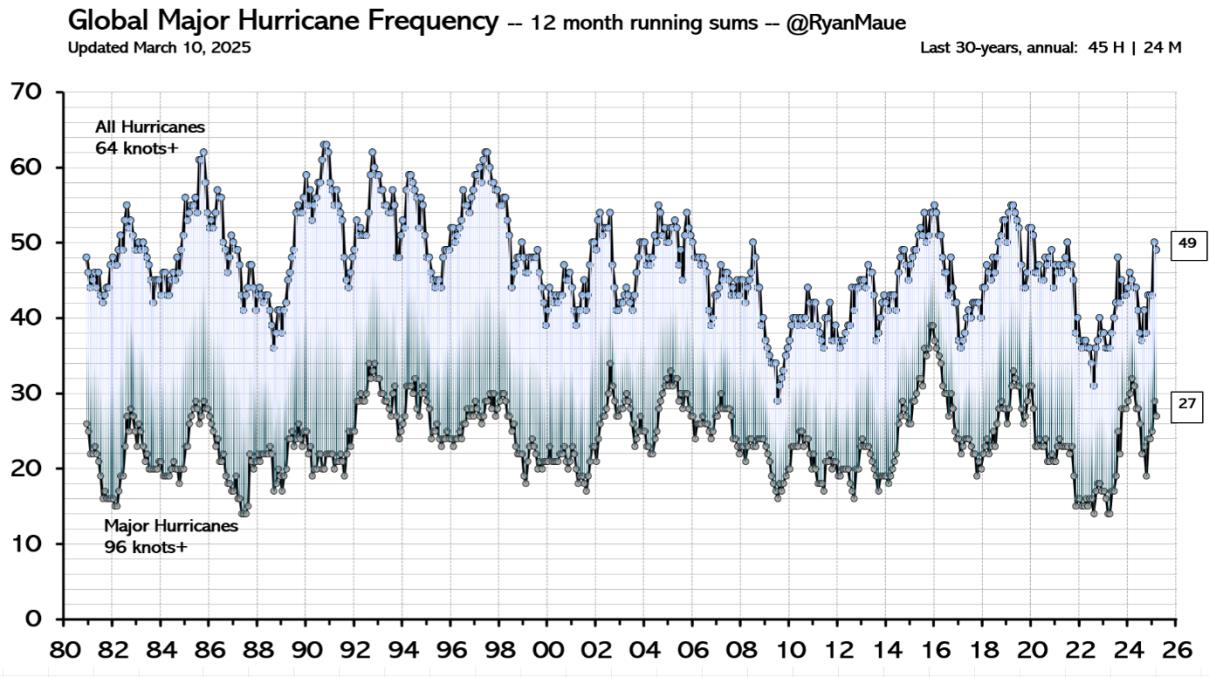
\includegraphics[width=1.0\textwidth]{bilder/bilderKlima-0037.jpg}\\[1cm]
\end{center}
\caption{Globale Häufigkeit von Hurrikans und schweren Hurrikans seit 1980. Quelle: Aktualisiert von Maue 2011.}
\end{figure}

Abbildung 6.2.2 zeigt die Häufigkeit atlantischer Hurrikans und schwerer Hurrikans (Kategorie 3 und höher) zurück bis 1920. Daten vor 1965 (dem Beginn der Satellitenbeobachtungen im Atlantik, blau schattiert) zeigen eine gewisse Unterzählung, wobei Daten vor 1920 erhebliche Unterzählung zeigen (Vecchi und Knutson, 2011). Alle Messgrößen atlantischer Hurrikan-Aktivität zeigen einen signifikanten Anstieg seit 1970. Jedoch sah der Zeitraum von 1971-1994 außergewöhnlich niedrige Aktivität, wobei hohe Aktivität (vergleichbar mit den letzten zwei Jahrzehnten, sogar bei Unterzählung) auch in den 1950er und 1960er Jahren und sogar in den 1930er Jahren beobachtet wurde.

\begin{figure}[H]
\begin{center}
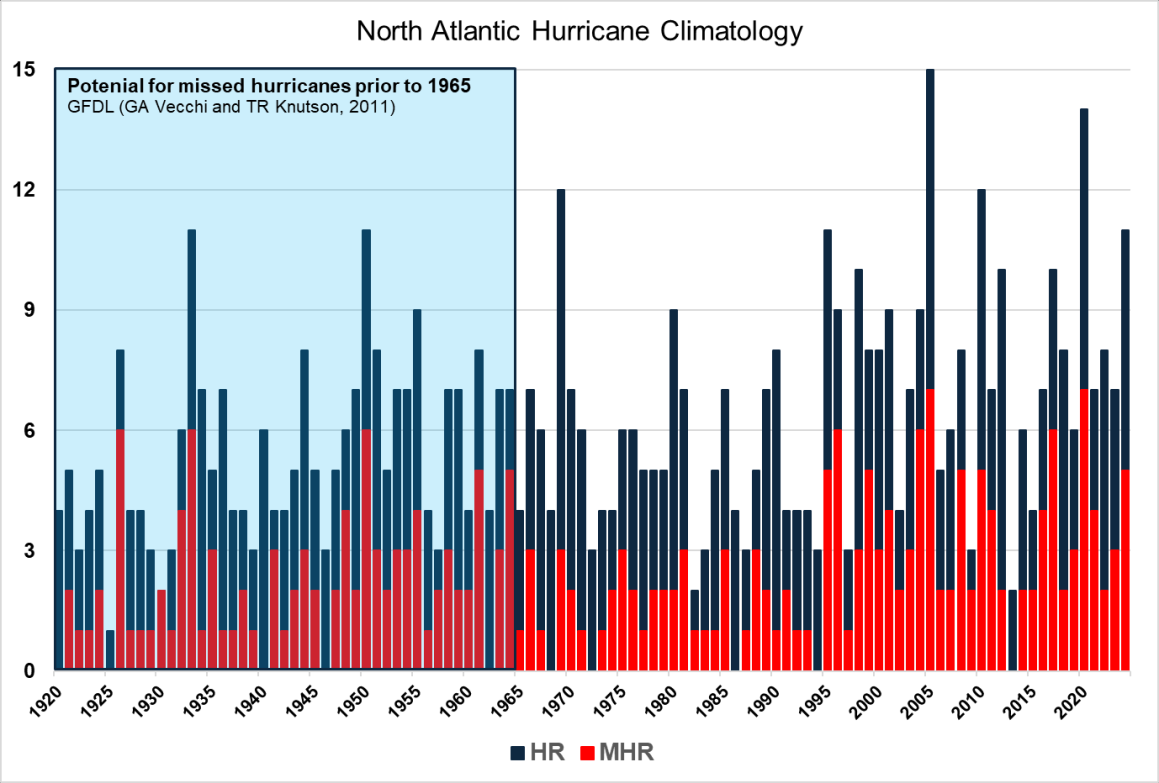
\includegraphics[width=1.0\textwidth]{bilder/bilderKlima-0038.png}\\[1cm]
\end{center}
\caption{Atlantische Häufigkeit von Hurrikans (HR) und schweren Hurrikans (MHR) seit 1920. Quelle: National Hurricane Center (2024)}
\end{figure}

Abbildung 6.2.2 zeigt, dass atlantische Hurrikans stark auf dekadischen und multidekadischen Zeitskalen variieren. Diese Variationen sind primär mit der Atlantischen Multidekadischen Oszillation (AMO) verbunden, die sich in beckenweiten Meeresoberflächentemperatur- und Meeresspiegel-Druckschwankungen manifestiert, die mit großräumigen Ozeanzirkulationsmustern verbunden sind. Die AMO befand sich während 1926-1970 und 1995-heute in ihrer warmen Phase, aber während 1971-1994 in ihrer kühlen Phase. Sie hat ihre größte Auswirkung auf die Anzahl schwerer Hurrikans (Kategorie 3+), die Goldenberg et al. (2001) mit übernormalen SSTs und verringerter vertikaler Scherung in der AMO-Warmphase in Verbindung brachten (siehe auch Bell und Chelliah, 2006; Klotzbach et al., 2018).

Klotzbach et al. (2018) führten eine umfassende Bewertung der auf Land treffenden Hurrikan-Daten für die kontinentalen USA seit 1900 durch. Abbildung 6.2.3 aktualisiert ihre Analyse bis 2024. Während die größten Zahlen landtreffender Hurrikans aus 2004, 2005 und 2020 stammen, gibt es keinen statistisch signifikanten Trend seit 1920. Abbildung 6.2.3 zeigt auch die Zeitreihe für schwere Hurrikan-Landtritte (Kategorie 3-5). Das größte Jahr in der Aufzeichnung ist 2005 mit 4 schweren Hurrikan-Landtritten. Jedoch gab es nach 2005 bis 2016 keine schweren Hurrikans, die die USA trafen - der längste solche Zeitraum seit 1920.

\begin{figure}[H]
\begin{center}
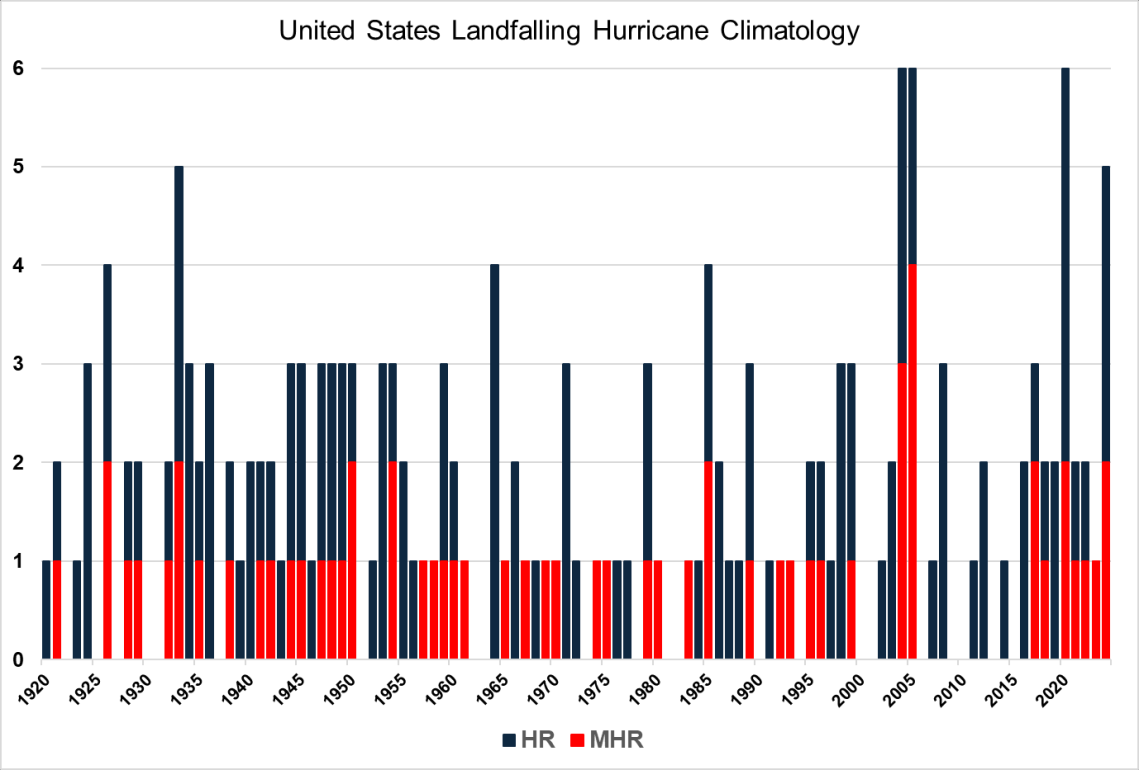
\includegraphics[width=1.0\textwidth]{bilder/bilderKlima-0040.png}\\[1cm]
\end{center}
\caption{US-Landtritt-Häufigkeit von Hurrikans (HR) und schweren Hurrikans (MHR) seit 1920. Quelle: NOAA HRD(a) (2024)}
\end{figure}

Abbildung 6.2.3 zeigt erhebliche zwischenjährliche bis multidekadische Variabilität in der US-Landtritt-Aktivität. Klotzbach et al. (2018) untersuchten, wie die Landtritt-Zahlen mit ENSO (El Niño versus La Niña) und den warmen versus kalten Phasen der Atlantischen Multidekadischen Oszillation (AMO) variieren.

Villarini et al. (2012) liefern eine Analyse der US-Hurrikan-Landtritte zurück bis 1878. Während es möglich ist, dass einige Landtritte im späten 19. Jahrhundert aufgrund dünn besiedelter Regionen an der Golfküste übersehen wurden, ist es bemerkenswert, dass das höchste Jahr in der gesamten Aufzeichnung 1886 ist, mit 7 Hurrikan-Landtritten, als menschliche Einflüsse auf das Klima viel geringer waren als heute.

Tabelle 6.2.1 zeigt die 10 stärksten Hurrikans (plus Gleichstände), die US-Landtritte machten. Von den Hurrikans, die mit anhaltenden Winden größer als 150 mph Landtritte machten, ist nur einer im 21. Jahrhundert aufgetreten.

Tabelle 6.2.1: Stärkste Hurrikans, die an der US-Küste Landtritte machten. Quelle: (NOAA HRD(b), 2024)


\begin{table}[htbp]
  \centering
  
  \label{tab:hurricans}
  \begin{tabular}{
      S[table-format=3.0]
      S[table-format=2.2]
      S[table-format=2.3]
      l
  }
    %\toprule
    {Rang} & {Jahr} & {Landtritt-Wind (MPH)} & {Name} \\
    \midrule
    1  &  1935 & 185 & \glqq Labor Day\grqq{} \\
    2  &  1969 & 175 & Camille \\
    3  &  1992 & 165 &  Andrew\\\
    4  &  2018 & 160 &  Michael \\
    5  &  1856 & 150 & \glqq Last Island\grqq{} \\
    5  &  1886 & 150 & \glqq Indianola\grqq{} \\
    5  &  1919 & 150 & ----- \\
    5  &  1932 & 150 & \glqq Freeport\grqq{} \\
    5  &  2004 & 150 & Charley\\
    5  &  2020 & 150 & Laura \\
    5  &  2021 & 150 & Ida \\
    5  &  2022 & 150 & Ian \\
    \bottomrule
  \end{tabular}
  \caption{Stärkste Hurrikans, die an der US-Küste Landtritte machten. Quelle: (NOAA HRD(b), 2024)}
\end{table}

Zusammenfassend liefern Analysen sowohl globaler als auch regionaler Variabilität und Trends der Hurrikan-Aktivität die Grundlage für die Erkennung von Veränderungen und das Verständnis ihrer Ursachen. Die relativ kurze historische Aufzeichnung der Hurrikan-Aktivität und die noch kürzere Aufzeichnung aus der Satellitenära reichen nicht aus, um zu bewerten, ob die jüngste Hurrikan-Aktivität ungewöhnlich im Verhältnis zur natürlichen Hintergrundvariabilität ist. Atlantische Hurrikan-Prozesse werden erheblich von natürlichen Modi der Ozeanzirkulationsvariabilität im Atlantik beeinflusst, insbesondere der Atlantischen Multidekadischen Oszillation. Während lange hypothetisiert wurde, dass eine steigende globale Meeresoberflächentemperatur eine Zunahme der Hurrikan-Intensität verursachen würde, wird die Identifikation eines signifikanten Trends in den Hurrikan-Daten durch eine kurze Datenaufzeichnung und erhebliche natürliche Variabilität behindert.

Prozessbasiertes Verständnis deutet auch darauf hin, dass Sturmfluten und Niederschläge von Hurrikans mit wärmeren Temperaturen zunehmen sollten. Jedoch verhindern die relativ kleine Anzahl von Hurrikans mit variierenden Landtritt-Orten und die komplexe Dynamik, die mit jedem Sturm verbunden ist, eine aussagekräftige Erkennung von Veränderungen.

\section{Temperaturextreme}
Die AR6-Bewertung konzentrierte sich auf den Zeitraum nach 1950 und berichtete über zunehmende Trends bei Hitzewellen-Häufigkeit und -Intensität. Jedoch stellte NCA4 fest, dass die Hitzewellen-Aktivität in den USA in den 1930er Jahren einen Höhepunkt erreichte (Abbildung 6.3.1).

\begin{quote}
AR6: Es ist praktisch sicher, dass heiße Extreme (einschließlich Hitzewellen) seit den 1950er Jahren häufiger und intensiver geworden sind in den meisten Landregionen, während kalte Extreme (einschließlich Kältewellen) weniger häufig und weniger schwerwiegend geworden sind (SPM, A3.1)

AR6: In Nordamerika gibt es sehr robuste Belege für eine sehr wahrscheinliche Zunahme der Intensität und Häufigkeit heißer Extreme und eine Abnahme der Intensität und Häufigkeit kalter Extreme für den gesamten Kontinent, obwohl es erhebliche räumliche und saisonale Variationen in den Trends gibt. Mindesttemperaturen zeigen eine konsistente Erwärmung über den gesamten Kontinent, während es kontrastierendere Trends bei den jährlichen maximalen Tagestemperaturen in Teilen der USA gibt. (Kapitel 11, S. 1550)

NCA4: Veränderungen bei warmen Extremen sind nuancierter als Veränderungen bei kalten Extremen. Zum Beispiel \textbf{stieg} die wärmste Tagestemperatur des Jahres in einigen Teilen des Westens über das vergangene Jahrhundert, aber es gab \textbf{Abnahmen} in fast allen Orten östlich der Rocky Mountains. Tatsächlich erlebten alle östlichen Regionen eine \textbf{Nettoabnahme}, am deutlichsten im Mittleren Westen (etwa 2,2°F [1,2°C]) und im Südosten (etwa 1,5°F [0,8°C]). (S. 190-191)

NCA4: Seit Mitte der 1960er Jahre gab es nur einen sehr geringen Anstieg der wärmsten Tagestemperatur des Jahres (inmitten großer zwischenjährlicher Variabilität). Hitzewellen (6-Tage-Perioden mit einer Maximaltemperatur über dem 90. Perzentil für 1961–1990) nahmen in der Häufigkeit bis Mitte der 1930er Jahre zu, wurden bis Mitte der 1960er Jahre erheblich seltener und nahmen danach wieder in der Häufigkeit zu. Wie bei warmen Tagestemperaturen \textbf{erreichte die Hitzewellen-Magnitude ein Maximum in den 1930er Jahren. (S. 190-191)}
\end{quote}

\begin{figure}[H]
\begin{center}
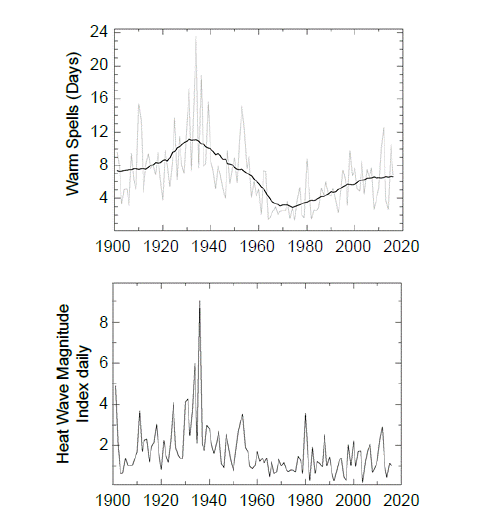
\includegraphics[width=1.0\textwidth]{bilder/bilderKlima-0042.png}\\[1cm]
\end{center}
\caption{US-Hitzewellen seit 1900. Quelle: NCA4 Abbildung 6.4}
\end{figure}

\subsection{Temperaturen in den USA werden weniger extrem}

Tägliche Maximaltemperaturen in der warmen Saison (Tmax, Mai-Sep) und tägliche Minimaltemperaturen in der kalten Saison (Tmin, Dez-Mär) sind verfügbar ab Dezember 1898 (126 Jahre). Der Datensatz besteht aus 1.211 CONUS-Stationen, die als United States Historical Climate Network oder USHCN-Stationen bezeichnet werden (siehe Abbildung 6.3.2; Quinlan et al. 1987, Karl et al. 1990). Diese Stationen wurden von NOAA als diejenigen mit den wenigsten problematischen Problemen mit Lücken, Stationsverlagerungen und Instrumentenänderungen ausgewählt. Wo Lücken noch bestehen, wurden nahegelegene Stationen (verzerrungskorrigiert) zusammengeführt, so dass das mittlere verfügbare Datenvolumen für eine Station 98\% beträgt. Obwohl es sicherlich Fehler im Datensatz gibt, einschließlich ungelöster unechter Erwärmung aufgrund von UHI-Effekten, die besonders Tmin-Aufzeichnungen verzerren, ist dieser Datensatz ausreichend genau für die Bewertung von Trends bei Tmax-Hitzeextremen.

\begin{figure}[H]
\begin{center}
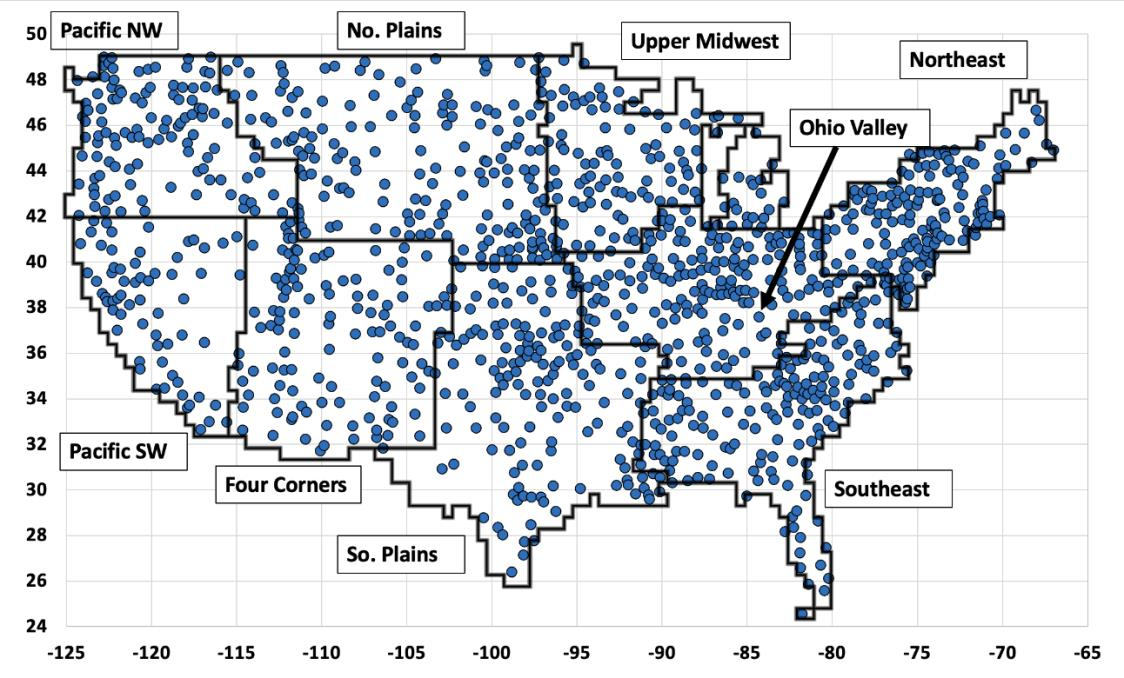
\includegraphics[width=1.0\textwidth]{bilder/bilderKlima-0043.jpg}\\[1cm]
\end{center}
\caption{Standorte der USHCN-Temperaturstationen. Quelle: USHCN.}
\end{figure}

Wir beginnen mit der Frage, ob das Auftreten täglicher Rekord-Hoch- oder Tieftemperaturen sich seit Dezember 1898 verändert hat. Jede warme Saison hat 153 Tage (1. Mai bis 30. Sep) und jede kalte Saison hat 122 Tage (1. Dez bis 31. Mär). Für jede Station und jeden Tag berechneten wir das Jahr, in dem die Rekord-Höchst- (niedrigste) Temperatur auftrat. Mit 126 Jahren Beobachtungen, wenn es keine Temperaturtrends über die Zeit gäbe, wäre die erwartete Anzahl von Rekorden für Tmax 1,21 (=153/126) pro Station pro Jahr und für Tmin 0,96 (=122/126) pro Station pro Jahr.

Abbildung 6.3.3 zeigt die beobachtete Verteilung in der Zeit des Auftretens dieser Extremereignisse. Es gibt ein gemeinsames Merkmal in vielen Metriken der warmsaisonalen Extreme in CONUS - die außergewöhnliche Hitze der 1920er und besonders der 1930er Jahre, mit einem Höhepunkt in 1936. Im Durchschnitt pro Station traten 60 Prozent der Tmax-Rekorde und 59 Prozent der Tmin-Rekorde in der ersten Hälfte des Zeitraums (1899-1961) auf.

\begin{figure}[H]
\begin{center}
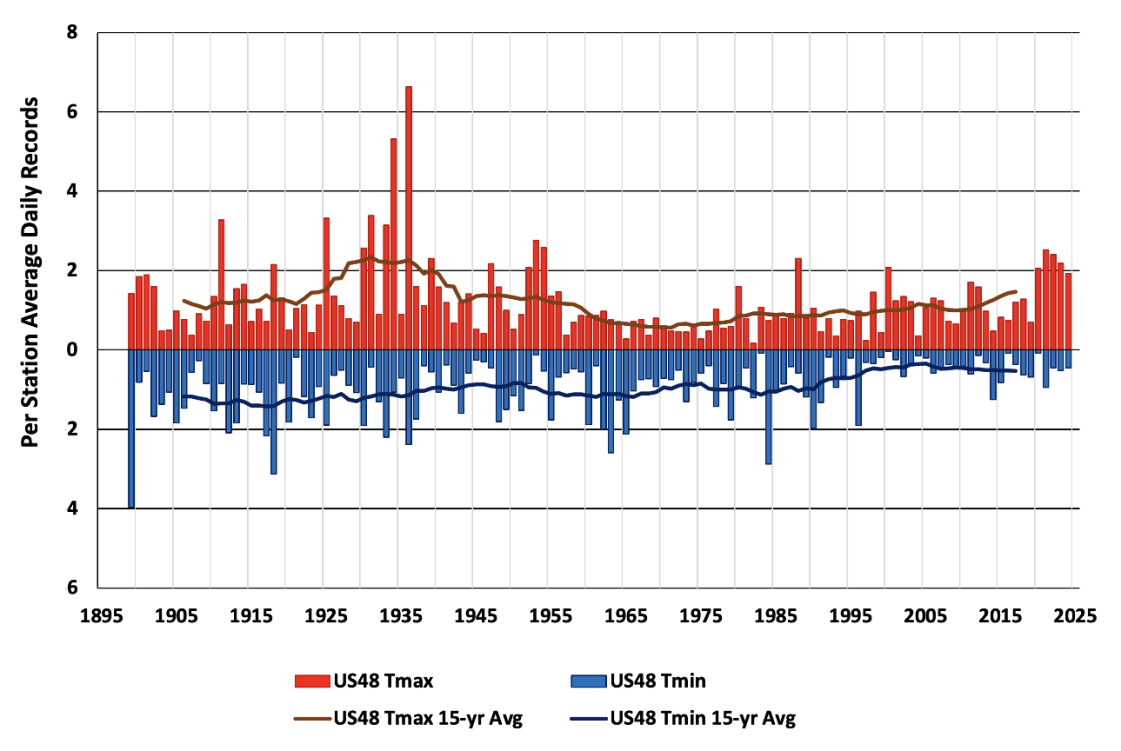
\includegraphics[width=1.0\textwidth]{bilder/bilderKlima-0044.png}\\[1cm]
\end{center}
\caption{Anzahl täglicher Rekord-Hoch- (rot) und Tieftemperaturen (blau) für warme und kalte Saisons in CONUS. Die Linien repräsentieren den 15-jährigen laufenden, zentrierten Durchschnitt. Quelle: 1.211 USHCN-Stationen, nach Bedarf ergänzt, um mindestens 92 Prozent der Beobachtungen in dem 126-jährigen Zeitraum seit Dezember 1898 zu erreichen. US48: zusammenhängende US-Staaten. Tmax: Maximaltemperatur. Tmin: Minimaltemperatur.}
\end{figure}

Auf der kalten Seite steht der Valentinstag-Arktisausbruch im Februar 1899 als das umfassendste Kälteextrem, das CONUS erlebte, mit 1917 an zweiter Stelle. Die Häufigkeit von Kälterekorden ist zurückgegangen, besonders im letzten Viertel des Zeitraums, in dem nur 13 Prozent der extremen Kälteereignisse gemessen wurden. Im Gegensatz dazu wurden 25 Prozent der extremen Tmax-Rekorde im letzten Viertel erreicht, in Übereinstimmung mit statistischen Erwartungen. Diese allgemeinen Merkmale wurden in früheren Bewertungen bemerkt (siehe oben, IPCC AR6, NCA4). Die Kombination der beiden Geschichten zeigt, dass die allgemeine Verringerung der Anzahl sowohl kalter als auch heißer Extreme über das vergangene Jahrhundert auf ein Klima hinweist, das weniger zu Extremen neigt.

Dieses Muster wird auch in Abbildung 6.3.4 gezeigt. Für jede Station und für jedes Jahr wurden die heißesten warmsaisonalen und kältesten kaltsaisonalen Temperaturen berechnet. Dann wurden die Unterschiede zwischen diesen nach Station berechnet und geografisch über alle Stationen gemittelt, was ein jährliches Maß für die erwartete Spanne lokaler Extremtemperaturen für jedes Jahr ergibt. Abbildung 6.3.4 zeigt den 15-jährigen nachlaufenden Durchschnitt dieses Maßes, der über das vergangene Jahrhundert deutlich zurückgegangen ist.

\begin{figure}[H]
\begin{center}
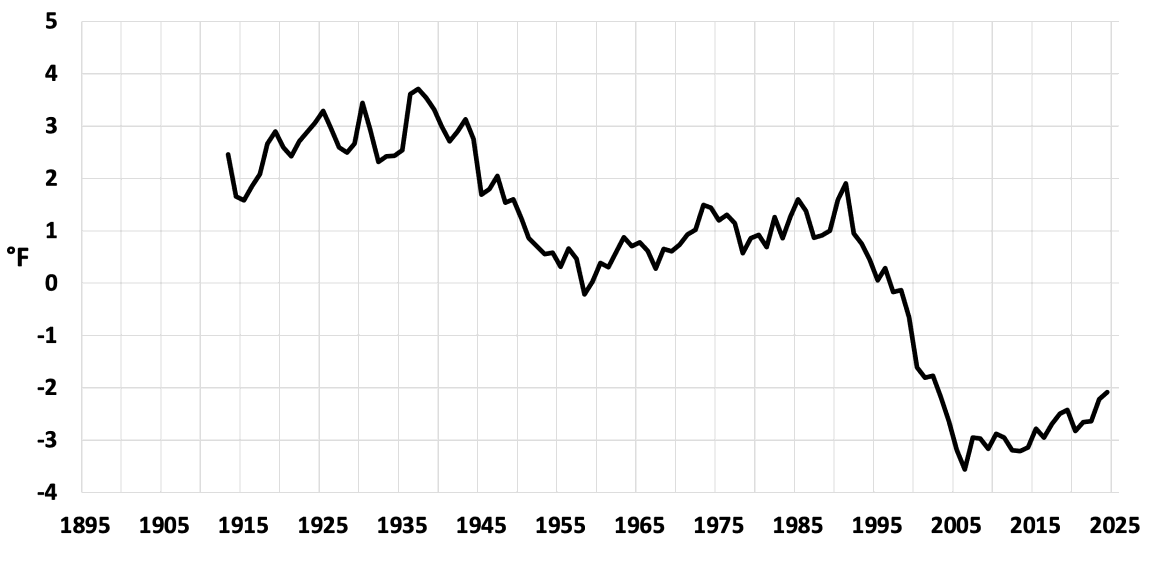
\includegraphics[width=1.0\textwidth]{bilder/bilderKlima-0045.png}\\[1cm]
\end{center}
\caption{15-jähriger nachlaufender Durchschnitt der Differenz jedes Jahres zwischen der heißesten warmsaisonalen Tmax und kältesten kaltsaisonalen Tmin jeder Station relativ zum langfristigen Durchschnitt. Quelle: Autoranalyse von USHCN-Daten.}
\end{figure}

Der durchschnittliche Unterschied für jede Station zwischen der heißesten Sommer-Tmax und kältesten Winter-Tmin ist in den letzten 126 Jahren um etwa \SI{5}{\degree\text{F}} zurückgegangen. Der Rückgang ist hauptsächlich auf wärmere Winter-Tmin zurückzuführen, aber auch ein Rückgang der Sommer-Tmax ist ein Faktor. Der Anstieg von Tmin war stark mit der wachsenden Präsenz von hergestellten Oberflächen um die Wetterstationen in den letzten 100+ Jahren verbunden (der sogenannte städtische Wärmeinseleffekt; Abschnitt 3.3, Karl et al. 1988, Runnals und Oke 2006, und Spencer et al. 2025).

Zusammenfassend zeigen langfristige Aufzeichnungen, während Temperaturextreme regelmäßig in den USA erlebt werden und große Medienaufmerksamkeit anziehen, dass das US-Klima über die Zeit weniger extrem (milder) geworden ist, wenn es durch die Spanne zwischen warmsaisonalen Maxima und kaltsaisonalen Minima gemessen wird.

\subsection{Überschreitungen einer Hitzeschwelle}
Unter der Überschrift \emph{Das Risiko von Temperaturextremen verändert sich} bemerkt der neueste US National Climate Assessment Report (NCA5) den Anstieg einer Schwellenwert-Metrik der Anzahl von Tagen bei oder über \SI{95}{\degree\text{F}} und stellt fest:
\begin{quote}
Die westlichen USA wurden seit den 1980er Jahren besonders von extremer Hitze betroffen..., mit einem größeren Anstieg von Tagen über \SI{95}{\degree\text{F}}, wie erwartet angesichts der größeren Erwärmung in dieser Region relativ zu den östlichen USA. Mehrere große Hitzewellen haben die USA seit 2018 betroffen, einschließlich eines rekordverschmetternden Ereignisses im pazifischen Nordwesten in 2021.
\end{quote}

Verändern sich die Auftreten von \SI{95}{\degree\text{F}}-Tagen? In einem so vielfältigen Klima wie dem von CONUS können Schwellenwert-Statistiken irreführend sein. Eine Region mit vielen Stationen, die nahe \SI{95}{\degree\text{F}} Tmax-Durchschnittstemperaturen im Sommer haben, könnte große Schwankungen in der Metrik sehen, wenn nur kleine Änderungen in der Durchschnittstemperatur auftreten. Anderswo, mit Stationen, die entweder selten oder praktisch immer \SI{95}{\degree\text{F}} Tmax-Temperaturen erreichen, wird eine kleine Änderung nicht viel Auswirkung auf die Ergebnisse haben.

\begin{figure}[H]
\begin{center}
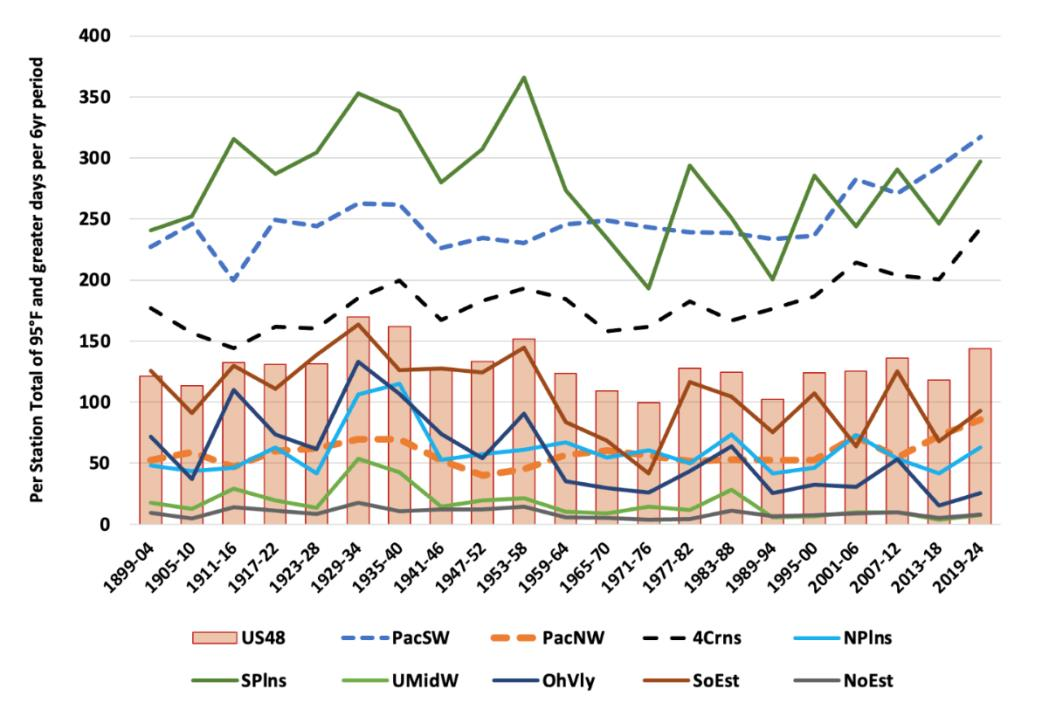
\includegraphics[width=1.0\textwidth]{bilder/bilderKlima-0046.jpg}\\[1cm]
\end{center}
\caption{Gesamtanzahl von Tagen $\geq$ \SI{95}{\degree\text{F}} in 6-jährigen Perioden, US 48 (Balken) und Regionen (Linien). Eine 6-Jahres-Periode wird verwendet, da dies die 126-jährige Aufzeichnung gleichmäßig teilt. Ergebnisse sind robust bei Verwendung von Perioden von 2 bis 11 Tagen. US48: zusammenhängende US-Staaten. Siehe Abbildung 6.3.2 für Regionsnamen. Quelle: Autoranalyse von USHCN-Daten.}
\end{figure}

In den letzten 126 Jahren erlebte die durchschnittliche CONUS-Station 129 Tage, die 95°F pro 6-Jahres-Periode überschritten, aber die regionalen Werte reichen von 278 in den Southern Plains bis 9 im Nordosten. Daher müssen solche Schwellenwert-Analysen mit Vorsicht interpretiert werden. Abbildung 6.3.5 zeigt, dass nur drei der neun Regionen, alle im Westen, aufwärts gerichtete Trends bei der Anzahl von 95°F oder heißeren Tagen erlebt haben (gestrichelte Linien). CONUS als Ganzes hat das nicht, und die anderen sechs Regionen haben Rückgänge erlebt.

Die pazifische Nordwest-Hitzewelle von 2021, die im NCA5-Zitat erwähnt wird, wird in Abschnitt 8.6.1 näher untersucht. Die Evidenz zeigt, dass es ein einzelnes, beispielloses Ereignis in der Aufzeichnung war, nicht Teil eines Musters zunehmender extremer Hitze. Zum Beispiel war die 5-Tage-Durchschnitts-Troposphären-Gitterpunkt-Temperaturanomalie über dem pazifischen Nordwesten während dieses Ereignisses +10,8°C, die extremste Sommer-Anomalie der nördlichen Hemisphäre an Gitterpunkten in den 46 Jahren aus über 4 Millionen Gitterwerten. Im Gegensatz dazu war die globale Temperaturanomalie während dieser Zeit praktisch null (+0,03°C, Mass et al. 2024).

\subsection{Hitzewellen}
Hitzewellen (aufeinanderfolgende Tage, die eine extreme Schwelle überschreiten) haben eine größere gesellschaftliche Auswirkung als eine einzelne tägliche Rekordtemperatur. Wir messen "Hitzewellen-Tage" hier als die Anzahl aller Tage im Mai-September jedes Jahres, die das 90. Perzentil für diesen Tag überschreiten und die innerhalb einer Periode von mindestens sechs aufeinanderfolgenden Tagen liegen. Dies entspricht der in NCA4 verwendeten Methode, außer dass der Referenzzeitraum hier die gesamte Aufzeichnung 1899-2024 ist, während NCA4 den Referenzzeitraum auf 1961-1990 kürzte, was ein kühles Intervall war. (Das unten gezeigte Ergebnismuster hängt nicht von der Wahl des Referenzzeitraums ab.) Diese Kürzung verstärkt positive Ergebnisse (Tage, die das 90. Perzentil überschreiten) in Jahren, die wärmer als der Referenzzeitraum sind, besonders ab 1960 bis zur Gegenwart (siehe Abbildung 6.3.6 und Diskussion unten).

\begin{figure}[H]
\begin{center}
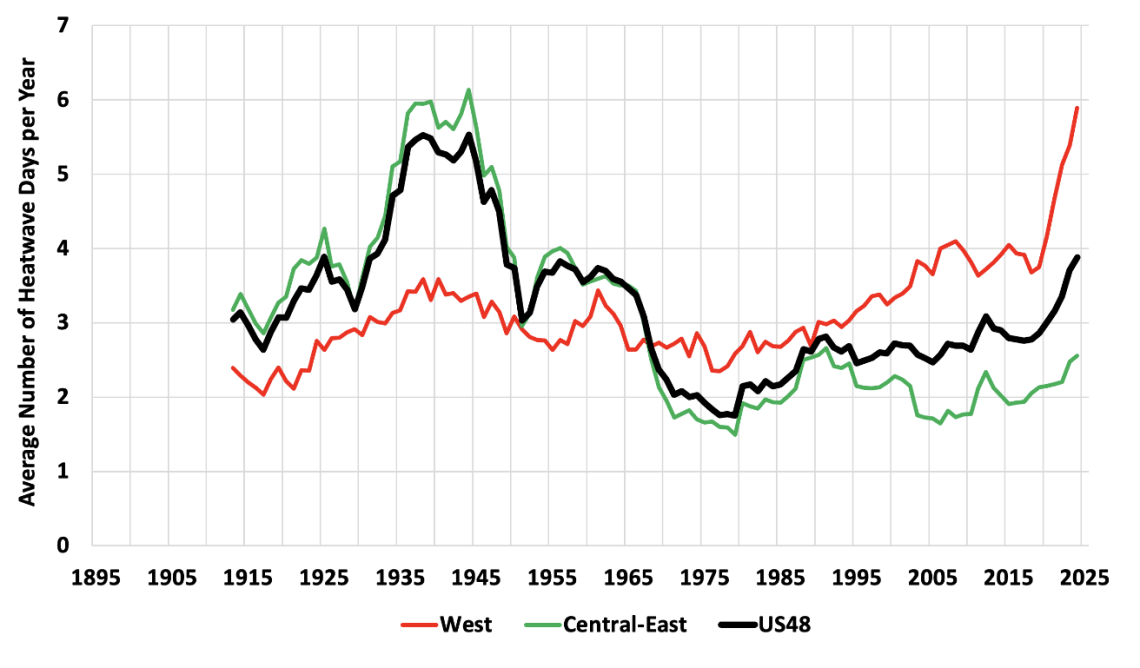
\includegraphics[width=1.0\textwidth]{bilder/bilderKlima-0047.png}\\[1cm]
\end{center}
\caption{15-jähriger nachlaufender Durchschnitt der Anzahl von Hitzewellen-Tagen pro Jahr pro Station in CONUS (schwarze Linie) und zwei Regionen: Westen (rot), Zentral-Osten (grün).}
\end{figure}

Abbildung 6.3.6 zeigt, dass es regionale Variationen in der Hitzewellen-Aktivität gibt. Die übermäßige Hitze der ersten Hälfte des 20. Jahrhunderts trat primär in den östlichen zwei Dritteln der Nation auf, während der Westen einen jüngsten Anstieg von Hitzewellen-Tagen gesehen hat (NCA5). Dies zeigt, dass die Hintergrund-Warmsaison-Zirkulation Hitzewellen in den östlichen Teilen des Landes in der ersten Hälfte des 20. Jahrhunderts begünstigte, aber im 21. Jahrhundert haben die Muster Hitzewellen im Westen begünstigt. Für CONUS als Ganzes sind Hitzewellen heute nicht häufiger als vor einem Jahrhundert, konsistent mit dem oberen Panel unserer Abbildung 6.4.1 aus NCA4.

Diese Metrik variiert erheblich mit der Region. Die vier nördlichen Regionen (Pacific NW, Northern Plains, Upper Midwest und Northeast) erleben im Durchschnitt 15 bis 27 Hitzewellen-Tage pro 15-Jahres-Periode. Im Gegensatz dazu sehen die fünf südlichen Regionen (Pacific Southwest, 4-Corners, Southern Plains, Ohio Valley und Southeast) 37 bis 54 solche Tage, im Wesentlichen doppelt so viele. Dies deutet darauf hin, dass das Sommer-Zirkulationsmuster in den südlichen Regionen anfälliger für stationäre Ereignisse ist, während transiente Systeme in den nördlichen Regionen häufiger sind und daher diese potenziell längeren Ereignisse verkürzen.

Die Analyse von Hitzewellen ist ein Beispiel dafür, warum es wichtig ist, vollständige Datensätze und angemessene Metriken zu betrachten. NCA5 leitet Leser zur Website https://www.globalchange.gov/indicators/heat-waves (USGCRP 2023), um eine Abbildung zu sehen, die die Anzahl städtischer Hitzewellen nach Jahrzehnten ab den 1960er Jahren zeigt, die wir als Abbildung 6.3.7 reproduzieren.

\begin{figure}[H]
\begin{center}
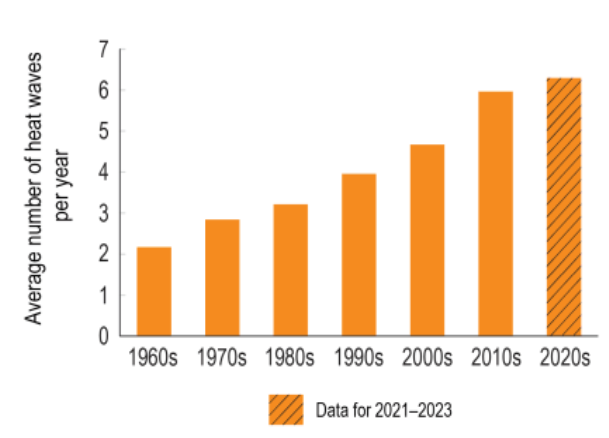
\includegraphics[width=1.0\textwidth]{bilder/bilderKlima-0048.png}\\[1cm]
\end{center}
\caption{Durchschnittliche Anzahl städtischer Hitzewellen pro Jahr für 50 große US-Metropolregionen, eine irreführende Metrik aus Gründen, die im Text erklärt werden. Von \url{https://www.globalchange.gov/indicators/heat-waves} (aufgerufen am 22. Mai 2025).}
\end{figure}

Die Abbildung zeigt einen monotonen Anstieg in jedem Jahrzehnt von zwei Auftreten pro Jahr in den 1960er Jahren auf sechs in den 2020er Jahren. Die verwendete Definition einer Hitzewelle ist ein ungewöhnliches, aber praktisches Maß menschlichen Unbehagens - eine Periode von mindestens 2 aufeinanderfolgenden Tagen, wenn die minimale scheinbare Temperatur (Kombination von Temperatur und Feuchtigkeit) das 85. Perzentil überschreitet. Beachten Sie auch, dass der Datensatz auf die 50 größten US-Städte beschränkt ist.

Angesichts der ungewöhnlichen Hitzewellen-Definition und des städtischen Fokus sind diese steigenden Werte seit 1960, die in USGCRP (2023) präsentiert werden, nicht informativ über langfristige Trends oder den Einfluss von THG-Emissionen aus mindestens zwei Gründen. Erstens, wie in Abbildungen 6.3.1 und 6.3.6 gezeigt, waren die 1960er Jahre das kälteste Jahrzehnt und die 1970er Jahre das zweitkälteste Jahrzehnt seit den 1910er Jahren, sodass dieses Startdatum die Zeitreihe darauf vorkonditioniert, Anstiege zu zeigen. Zweitens ist die Urbanisierung nach 1960 in diesen Städten ein Hauptfaktor für den Anstieg von Tmin relativ zu ko-lokalisierten Tmax und relativ zu Tmin an nahegelegenen ländlichen Stationen (Karl et al. 1988, Runnals und Oke 2006, Christy et al. 2009, McNider et al. 2012). Dies schmälert nicht den realen Anstieg der nächtlichen Temperaturen in großen US-Städten und die gesellschaftlichen Auswirkungen, die mit diesen Änderungen verbunden sind. Jedoch bemerken wir aus verschiedenen Gründen, dass Sommer-Tmax (besonders in ländlichen Gebieten) eine bessere Metrik für die Erkennung von Änderungen in Hitzewellen ist, die von Änderungen im Hintergrundklima beeinflusst werden, zum Beispiel aufgrund steigender THGs (Christy et al. 2009). Für CONUS als Ganzes deutet die Evidenz in diesem Abschnitt darauf hin, dass THG-Emissionen wenig bis keine Auswirkung auf Hitzewellen vor dem Hintergrund von Urbanisierung und natürlicher Klimavariabilität hatten. Unabhängig von der ultimativen Ursache regionaler Trends haben Hitzewellen wichtige Auswirkungen auf die Gesellschaft, die angegangen werden müssen, wie wir in Kapitel 10 diskutieren.

\begin{fullbox}{BOX: Gefahren kurzer Datenaufzeichnungen}
% --- Oberer (fließender) Teil: darf über mehrere Seiten laufen ---
San Francisco bietet eine gute Fallstudie der Begrenzung der Verwendung kurzer historischer Stichproben zur Charakterisierung natürlicher Variabilität von Extremereignissen. Angenommen, wir verwenden eine 130-jährige Stichprobe täglicher San Francisco-Niederschläge von 1895 bis 2024 und wir suchen nach 3-Tage-, 5-Tage-, 14-Tage- und 30-Tage-Niederschlagsrekorden. Die Ergebnisse sind wie in Tabelle 6.2 gezeigt.

\begin{center} 
  \begin{tabular}{
       l
       S[table-format=2.2]
       S[table-format=4.0]
   }
  \toprule
  \multicolumn{1}{l}{Ereignis} & 
  \multicolumn{1}{c}{Rekord (Zoll)} & 
  \multicolumn{1}{c}{Jahr} \\
  \midrule
     3-Tage   &  6.94 & 2023 \\
     5-Tage   &  8.55 & 2023 \\
    14-Tage   & 12.62 & 2023 \\
    30-Tage   & 18.93 & 1998 \\
  \bottomrule
  \end{tabular}
  \captionof{table}{Extreme Niederschlagsrekorde, San Francisco, 1895–2024.}
  \label{tab:box2table1}
\end{center}

Die Rekorde gruppieren sich alle in den jüngeren Jahren. 2023 scheint ein außergewöhnliches Jahr zu sein, und da es nahe dem Ende der Stichprobe liegt, könnte es darauf hindeuten, dass das Klima in einen gefährlicheren Zustand gewechselt ist, vielleicht aufgrund menschlicher Einflüsse. [Hinweis: "2023" zeigt an, dass das Ereignis im Wasserjahr von Aug 2022 bis Juli 2023 auftrat.]

Aber das Bild ist sehr anders, wenn wir eine Stichprobe verwenden, die 45 Jahre früher beginnt, in 1850. Tabelle 6.3 zeigt, dass die rekordschaffenden Ereignisse alle in den 1860er Jahren passierten. Außerdem ist 2023 jetzt nicht einmal an zweiter Stelle, sondern fällt auf den 3. oder 4. Platz. Und ein Vergleich der Rekorde der beiden Tabellen zeigt, dass die extremen Niederschlagsereignisse in 1862 und 1867 erheblich mehr Niederschlag beinhalteten als die Ereignisse von 1998 und 2023, mit 14- und 30-Tage-Summen etwa 50 Prozent höher.

\noindent
\noindent
\begin{minipage}{\textwidth}
\begin{center}
  \begin{tabular}{
        l
        S[table-format=2.2]
        S[table-format=4.0]
        >{\centering\arraybackslash}p{5.5cm}
  }
    \toprule
    \multicolumn{1}{l}{Ereignis} &
    \multicolumn{1}{c}{Rekord (Zoll)} &
    \multicolumn{1}{c}{Jahr} &
    \makecell{Rang des 130-Jahresextrems\\ aus Tabelle 6.2} \\
    \midrule
    3-Tage   &  8.85 & 1867 & 3 \\
    5-Tage   &  9.80 & 1867 & 3 \\
    14-Tage  & 19.05 & 1862 & 4 \\
    30-Tage  & 28.25 & 1862 & 2 \\
    \bottomrule
  \end{tabular}
  \captionof{table}{Extreme Niederschlagsrekorde, San Francisco, 1850–2024.}
  \label{tab:box2tab2}
\end{center}
\end{minipage}


% --- Unterer Teil: wird ans Boxende (letzte Seite) gesetzt ---
Die Spanne natürlicher Variabilität wird noch bemerkenswerter, wenn paläoklimatische Evidenz untersucht wird. Porter et al. (2011) entdeckten, dass in den letzten 1.800 Jahren mindestens sechs Megastürme intensiver waren als der verheerende 1861-62 ARkStorm, der die Region traf.

Dieses Beispiel illustriert die Begrenzungen der Verwendung relativ kurzer Klimazeiträume (~130 Jahre) zur Bewertung des Charakters und der Spanne natürlicher Variabilität im Allgemeinen und von Extremereignissen im Besonderen. Eine genaue Darstellung der vollen Spanne natürlicher Variabilität ist notwendig für jede Attributionsanalyse (Abschnitt 8.6). Infrastrukturplaner, Notfallmanagement-Institutionen und Attributionswissenschaftler würden die erhebliche Falschdarstellung der Magnitude eines zukünftigen Extrems verstehen, wenn sie nur auf den letzten 130 Jahren basiert. In diesem Fall liefert eine einzelne Zeitstichprobe von 130 Jahren eine Unterschätzung des Extremwertes um bis zu 50 Prozent, die bestimmt wird, wenn nur 45 weitere Jahre von Beobachtungen hinzugefügt werden. Verglichen mit paläoklimatischer Evidenz auf Jahrtausend-Skala würde eine noch größere Unterschätzung auftreten. Eine wichtige Lehre ist, dass das Klima große Überraschungen von sich aus liefern kann, sogar ohne menschliche Einflüsse.
\end{fullbox}

\section{Extreme Niederschläge}
AR6 bewertete, dass eine Zunahme starker Niederschläge in Daten ab den 1950er Jahren beobachtet wurde.
\begin{quote}
AR6: Die Häufigkeit und Intensität starker Niederschlagsereignisse haben seit den 1950er Jahren über den meisten Landgebieten zugenommen, für die Beobachtungsdaten für Trendanalysen ausreichend sind (hohes Vertrauen). (SPM A3.2)

AR6: In Nordamerika gibt es robuste Evidenz, dass die Magnitude und Intensität extremer Niederschläge seit den 1950er Jahren sehr wahrscheinlich zugenommen hat. Sowohl [Ein-Tages-Maxima] als auch [5-Tages-Maxima] haben in Nordamerika während 1950-2018 signifikant zugenommen. (Kapitel 11, S. 1560)
\end{quote}

Die US National Climate Assessments (NCA4, NCA5) haben eine Zunahme des Auftretens der stärksten Niederschlagsereignisse (auf verschiedene Weise definiert) primär in der östlichen Hälfte von CONUS hervorgehoben, besonders im Nordosten, wenn die Analyse entweder 1901 oder 1958 beginnt. Interessanterweise zeigen die regionalen Variationen, dass die größten Zunahmen extremer Niederschlagsereignisse im Nordosten und die kleinsten im Westen auftreten, ein Muster entgegengesetzt zu den Änderungen bei Temperaturextremen (Abbildung 6.3.6).

McKitrick und Christy (2019) untersuchten langfristige und konsistente Stationsbeobachtungen extremer täglicher Niederschläge, um einige dieser NCA-Behauptungen für den Südosten und die Westküste zu testen, unter Verwendung eines Trendmodells mit einem nichtparametrischen Varianzschätzer, der robust gegen die komplexen Autokorrelationseigenschaften von Niederschlagsdaten ist. Als die Zeitreihen zeitlich zurück verlängert wurden (in einigen Fällen bis 1872) oder später begannen (1978), gab es keine signifikanten Trends für beide Regionen.

Diese Befunde wurden für diesen Bericht aktualisiert (McKitrick und Christy 2025) mit ähnlich konstruierten Beobachtungen von 29 Stationen an der pazifischen CONUS-Küste (1893ff von San Diego CA bis Blaine WA) und 24 Stationen im feuchten Südosten (1872ff von Austin TX bis Washington DC), sowie der Hinzufügung von 27 Stationen im Nordosten (1888ff von Buffalo NY bis Eastport ME). Die Standorte sind in Abbildung 6.4.1 gezeigt. Die Stationen wurden basierend auf der Verfügbarkeit langfristiger hochwertiger Aufzeichnungen ausgewählt. Die Regionen sind jeweils mit wichtigen Merkmalen extremen Niederschlagsverhaltens verbunden: die Pazifikküste ist mit landtreffenden atmosphärischen Flüssen verbunden, für die AR6 Evidenz zunehmender Aktivität seit 1948 mit weiteren Zunahmen anführt, die erwartet werden, während sich die Welt erwärmt (AR6 8.3.2.8.2); der NCA-Bericht zeigt, dass der Nordosten die größte Zunahme extremer Ereignisse erlebt hat, und der Südosten ist ebenfalls ein Ort, der in den NCAs als mit zunehmenden extremen Ereignissen vermerkt wird.

Die Ergebnisse der Anwendung der Analyse von McKitrick und Christy (2019) waren wie folgt für jede Region, gefolgt von weiterer Erklärung.
Abbildung 6.4.1: Standorte der Niederschlagsüberwachungsstationen, die in diesem Bericht verwendet werden. Orange: Pazifikküste. Blau: Nordosten. Grün: Südosten. Daten von McKitrick und Christy (2025).


\textbf{Starke Niederschlagsereignisse an der Pazifikküste}
\begin{itemize}
\item Der durchschnittliche Niederschlagstrend ist statistisch signifikant (abwärts) in Astoria OR; anderswo nicht signifikant. 
\item Der Trend in der Niederschlagsvarianz ist positiv und signifikant in Big Sur CA; anderswo nicht signifikant. 
\item Der Trend im täglichen maximalen Niederschlag ist positiv und signifikant in Aberdeen WA und Big Sur CA und negativ und signifikant in Newport OR (anderswo nicht signifikant). 
\item Gemittelt über alle Stationen in der Region ist keiner dieser drei Trendparameter statistisch signifikant.  
\end{itemize}

Die Pazifikküste erhält beträchtliche Niederschläge von Atmospheric River (AR) Ereignissen, die oft mehr als ein oder zwei Tage dauern (z.B., Gershunov et al. 2017, Pan et al. 2024). Die schlimmste Serie solcher Ereignisse in der jüngeren Geschichte war der sogenannte ARkStorm, der im Dezember 1861 und Januar 1862 auftrat; er schüttete fast 10 Fuß Regen in Teilen Kaliforniens aus und tauchte das gesamte Central Valley wochenlang unter bis zu 15 Fuß Wasser (Brewer 1930, Null und Hulbert 2007). Zusätzlich hat paläoklimatische Forschung sechs Megastürme gefunden, die schwerwiegender waren als 1861–1862 in Kalifornien während der letzten 1800 Jahre, auftretend in Intervallen von etwa 300 Jahren (Porter et al. 2011).

\begin{figure}[H]
\begin{center}
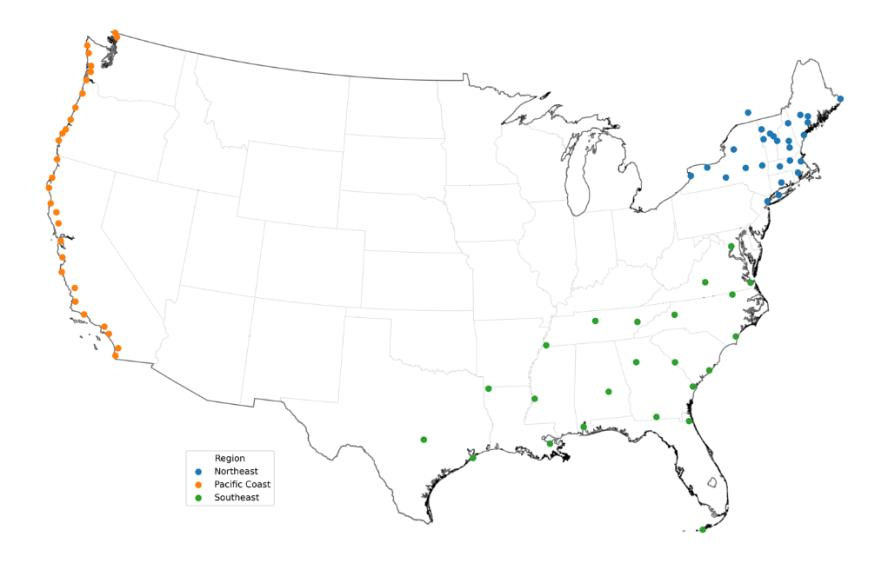
\includegraphics[width=1.0\textwidth]{bilder/bilderKlima-0055.jpg}\\[1cm]
\end{center}
\caption{Standorte der in diesem Bericht verwendeten Niederschlagsmessstationen.
Orange: Pazifikküste. Blau: Nordosten. Grün: Südosten. Daten von McKitrick und
Christy (2025).}
\end{figure}

Wir untersuchen Auftreten von 5-Tage-Wassermassen wie folgt. Die Pazifikküste als Beispiel nehmend, enthält eine 130-jährige Spanne 26 5-Jahres-Intervalle. An jedem Standort berechneten wir die 5-Tage-Niederschlagssummen das ganze Jahr über und wählten die 26 höchsten Werte über die Stichprobe aus. Ein einzelnes Jahr könnte mehr als eines der 26 schwersten haben. Jedes davon kann als 1-in-5yr-Ereignis betrachtet werden. Wenn es keine Trends im Niederschlag gibt, dann sollte die Gesamtzahl dieser Ereignisse über alle Stationen gleichmäßig über die Jahre verteilt sein. In Abb. 6.4.2 zeigen wir die Verteilung in der Zeit dieser Ereignisse für die Pazifikküste. Die Wassermassen, die mit dem massiven 1997-98 El Niño-Ereignis verbunden sind, sind leicht erkennbar. Während unregelmäßig, wie typisch für solche Niederschlagsmetriken, gibt es keine Anzeichen einer Tendenz, über die Zeit häufiger zu werden.

\begin{figure}[H]
\begin{center}
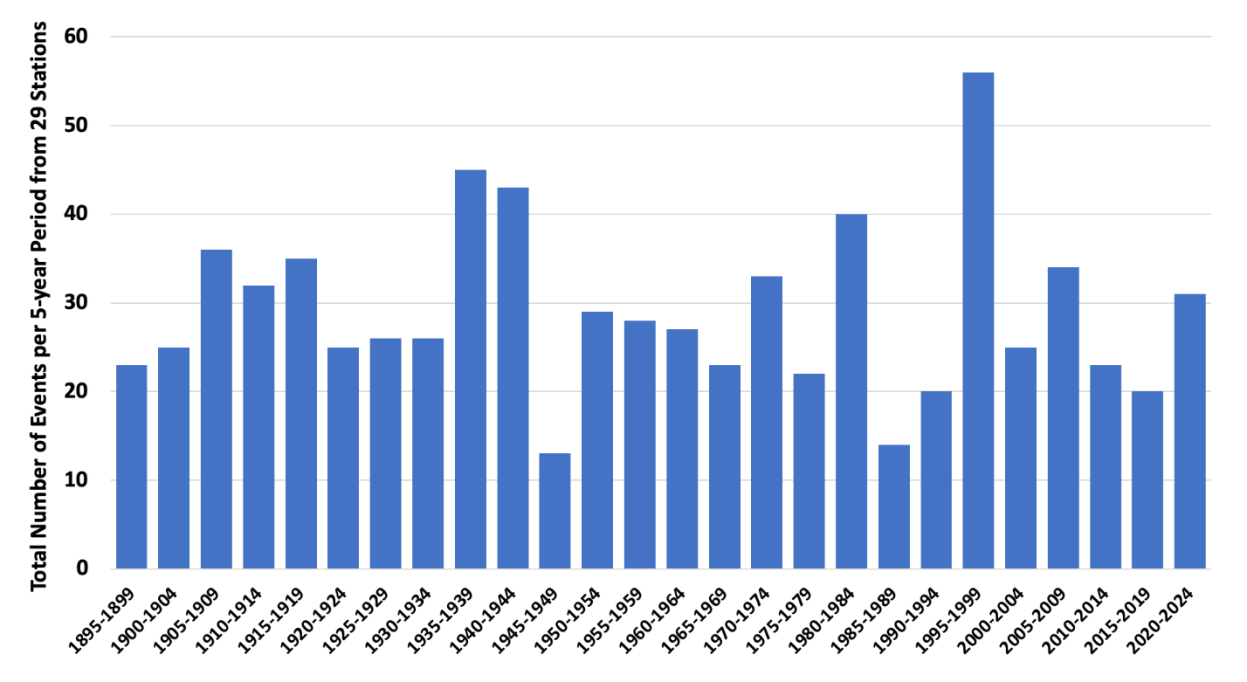
\includegraphics[width=0.9\textwidth]{bilder/bilderKlima-0056.png}\\[1cm]
\end{center}
\caption{Die Zeitverteilung in 5-Jahres-Perioden der 26 schwersten (1-in-5 yr) Auftreten für 29 Stationen an der Pazifikküste.}
\end{figure}
\begin{figure}[H]
\begin{center}
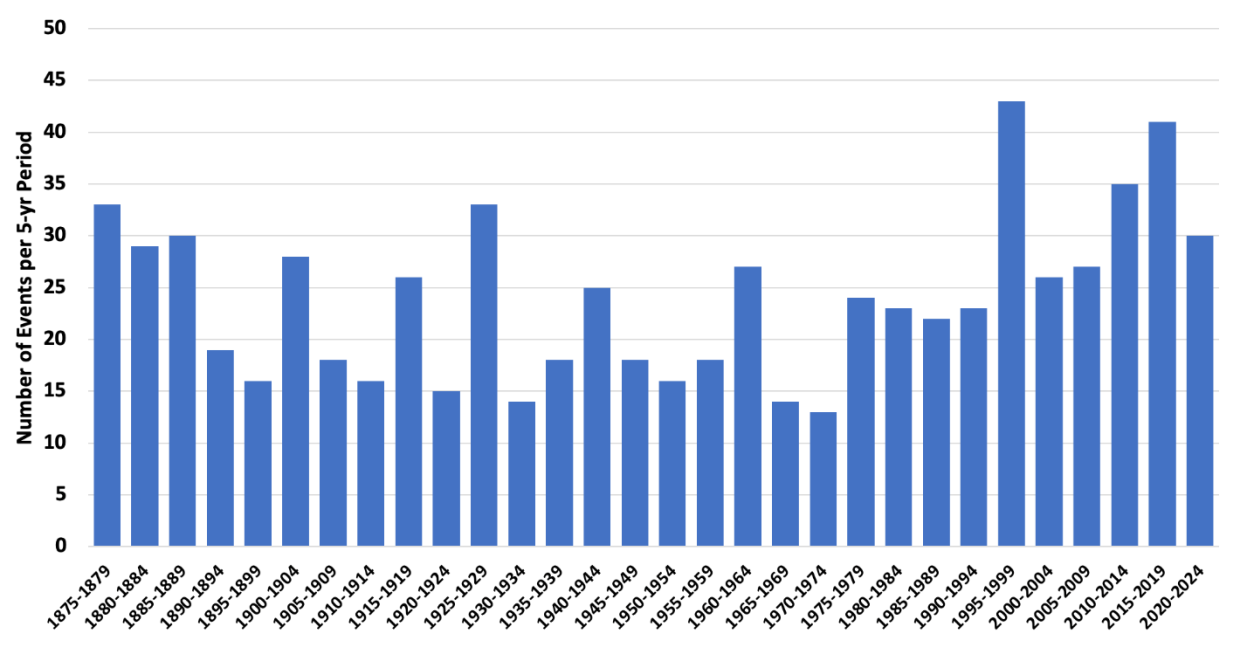
\includegraphics[width=0.9\textwidth]{bilder/bilderKlima-0057.png}\\[1cm]
\end{center}
\caption{Wie in Abb. 6.4.2, jedoch für die 30 schwersten Ereignisse (1-in-5-Jahre) für 24 Stationen im feuchten
Südosten von Austin, Texas, bis Washington, D.C., in 5-Jahres-Intervallen für den Zeitraum 1875–2024.}
\end{figure}

\textbf{Starke Niederschlagsereignisse im Südosten}
\begin{itemize}
\item Der Trend im durchschnittlichen Niederschlag ist positiv und statistisch signifikant in Mobile AL und Quitman GA, aber anderswo nicht signifikant. 
\item Der Trend in der Niederschlagsvarianz ist positiv und signifikant in Mobile AL, aber anderswo nicht signifikant.
\item Der Trend im täglichen maximalen Niederschlag ist positiv und signifikant in Vicksburg MS und Norfolk VA, aber anderswo nicht signifikant.
\item Gemittelt über alle Stationen in der Region ist keiner dieser drei Trendparameter statistisch signifikant. 
\end{itemize}

Abbildung 6.4.3 ist analog zu Abbildung 6.4.2 für die letzten 150 Jahre in der feuchten Südost-Zone. Das zeitliche Muster der 5-Tage-Summen der 1-in-5yr schweren Ereignisse ist allgemein unauffällig, obwohl eine Häufung höherer Werte von 1995 bis 2019 erscheint. Die Zunahme in diesen Jahren ist größtenteils auf die 4 nordöstlichsten Stationen von Wilmington NC, Weldon NC, Washington DC und Norfolk VA zurückzuführen. Dies bestätigt das in NCA4 und NCA5 angedeutete Muster -- eine zunehmende Häufigkeit schwerer Ereignisse aufgrund einer zeitlichen Häufung tropischer Stürme von Ost-NC bis Maine, die unten diskutiert wird. Ansonsten zeigen die verbleibenden 20 Stationen eine unauffällige zeitliche Verteilung schwerer Ereignisse.

\textbf{Starke Niederschlagsereignisse im Nordosten}
\begin{itemize}
\item Der Trend im durchschnittlichen Niederschlag ist positiv und statistisch signifikant in 12 von 27 Standorten und auch im regionalen Durchschnitt. 
\item Der Trend in der Niederschlagsvarianz ist positiv und signifikant in Portland ME, Albany NY, Buffalo NY und Eastport ME, aber anderswo nicht signifikant. 
\item Der Trend im täglichen maximalen Niederschlag ist positiv und signifikant in Portland ME, Gardiner ME und Eastport ME, aber anderswo nicht signifikant. 
\item Wenn über alle Stationen in der Region gemittelt, gibt es keinen statistisch signifikanten Trend in entweder der Niederschlagsvarianz oder dem Maximum. 
\end{itemize}




Abb. 6.4.4 ist analog zu Abbildung 6.4.2 für die letzten 135 Jahre in 27 Stationen im Nordosten (einschließlich Montreal Kanada). Wir verwenden hier 3-Tage-Summen, da dies die größten zeitlichen Variationen in der Zeit produzierte. In dieser Region treten 77 Prozent der Ereignisse während Juni bis Oktober auf und werden von Einbrüchen von Hurrikans, tropischen Stürmen oder tropischen Stürmen dominiert, die zu außertropischen Systemen übergehen. Laut NCA4 und NCA5 erlebte diese Region die größten Zunahmen extremer Ereignisse, sodass sie eine nähere Untersuchung verdient.

Es gibt eine bemerkenswerte Häufung extremer Ereignisse von 1995 bis 2014. Howarth et al. (2019) untersuchten eine ähnliche Region wie in Abb. 6.4.4, die PA und NJ einschließt, und berichteten signifikante Unterschiede in verschiedenen Niederschlagsextremen zwischen zwei 18-Jahres-Perioden, 1979-96 und 1997-2014. Das schloss eine 317-prozentige Zunahme von 24-Stunden-Ereignissen ein, die 6 Zoll überschreiten, während wir eine 58-prozentige Zunahme über dieselben Jahre finden. Jedoch zeigt Abbildung 6.4.4, dass die Häufigkeit nach 2014 scharf abfällt und in den nachfolgenden 5-Jahres-Intervallen zum langfristigen Durchschnitt zurückkehrt, was wiederum die Gefahren des Ziehens von Schlüssen aus kurzfristigen Trends in hochvariablen Metriken illustriert.

\begin{figure}[H]
\begin{center}
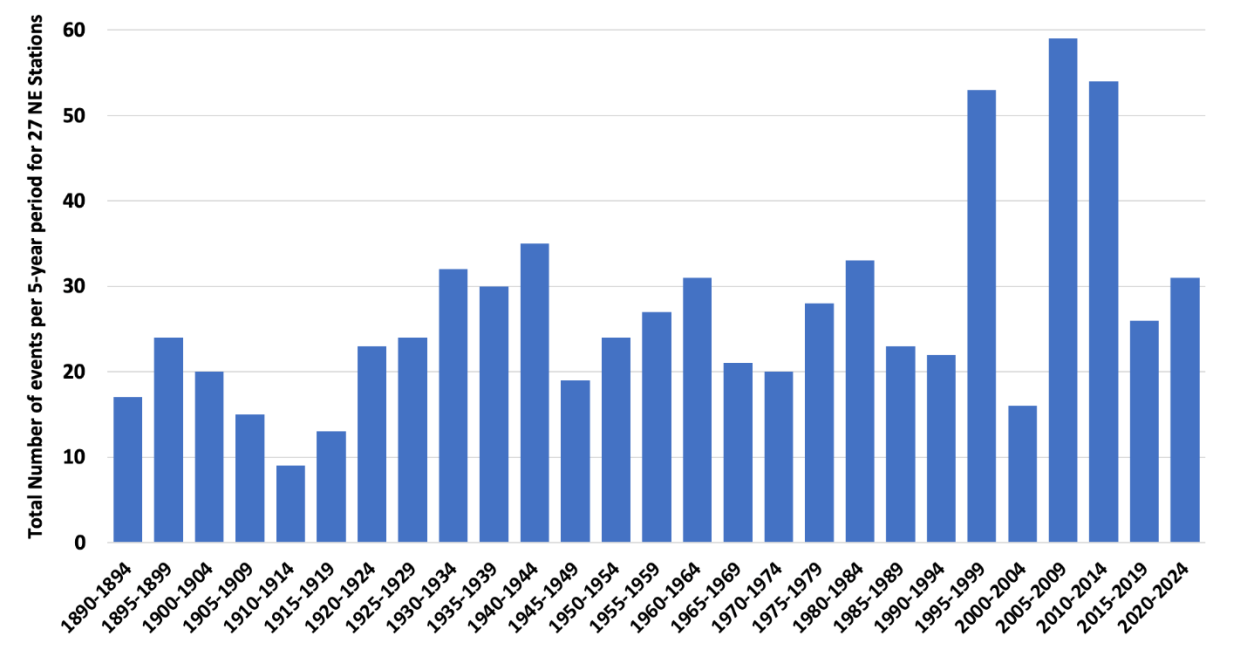
\includegraphics[width=0.9\textwidth]{bilder/bilderKlima-0058.png}\\[1cm]
\end{center}
\caption{Wie in Abb. 6.4.2, aber für die schwersten 27 (1-in-5yr) 3-Tage-Niederschlagsereignisse für 27 Nordost-Stationen von NY bis ME, einschließlich Montreal.}
\end{figure}
\begin{figure}[H]
\begin{center}
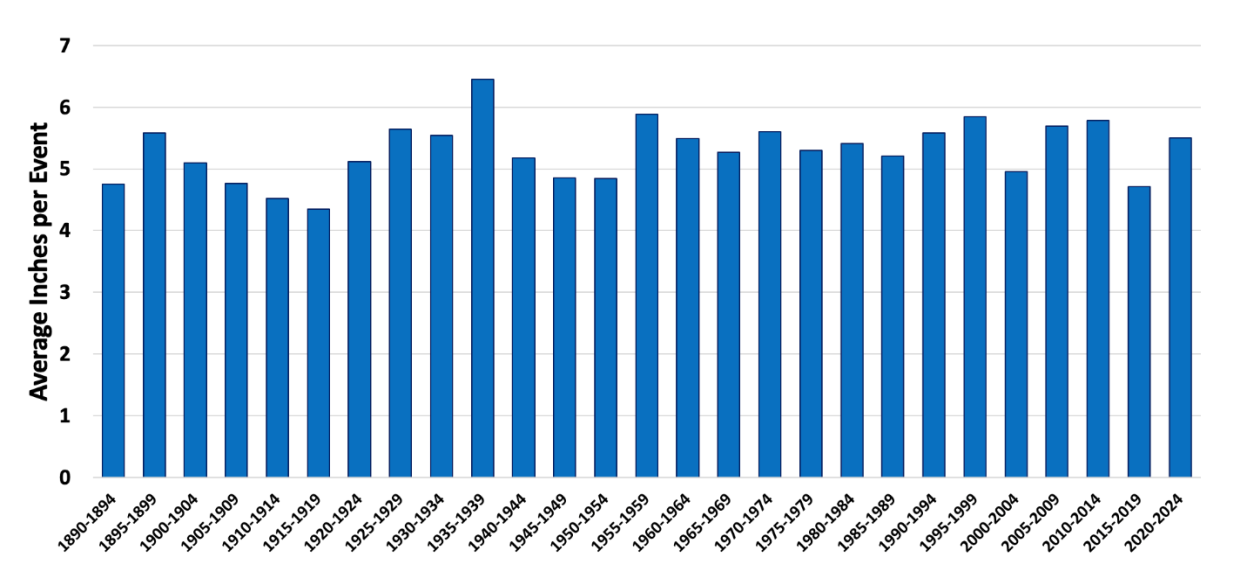
\includegraphics[width=0.9\textwidth]{bilder/bilderKlima-0059.png}\\[1cm]
\end{center}
\caption{Durchschnittliche Niederschlagsmenge, die in den 1-in-5yr-Ereignissen für die NE-Stationen fällt.}
\end{figure}

Die hohe prozentuale Zunahme in der Howarth et al. Stichprobe ist mit kleinen Zahlen an relativ wenigen Standorten verbunden: es gab nur 6 in der ersten Periode und 25 in der zweiten über 58 Stationen. Die meisten Stationen verzeichneten kein solches Ereignis. Wenn es eine regionsweite Zunahme schwerer Ereignisse gibt, sollte sie im Durchschnitt über alle Stationen gesehen werden. Abbildung 6.4.5 zeigt den durchschnittlichen Niederschlag in den 1-in-5 yr-Ereignissen über den NE. Der Trend ist nur +0,04 Zoll/Dekade. Die höchste Menge, 1935-39, schließt den Great New England Hurricane von 1938 ein, einen der seltenen schweren (Kategorie 3 oder höher) Hurrikans, die die Region trafen.

Die Ergebnisse in Abbildungen 6.4.4 und 6.4.5 deuten daher darauf hin, dass obwohl es einen Anstieg in der Anzahl von Ereignissen an wenigen Standorten während des 1995 bis 2014 Intervalls gab, gab es kein regionales Muster und die Änderung hielt nicht über 2014 hinaus an.

Jong et al. (2024) dokumentieren die Zunahme tropischer Einflüsse auf Niederschlagsereignisse im Nordosten seit 1959 und schlossen: "Der Herbst-Extremniederschlagstrend über den Nordosten der USA wird primär tropischen Wirbelsturm-verwandten Ereignissen seit den 1990er Jahren zugeschrieben." Die Frage wird dann: "War die zeitliche Häufung tropischer Systeme in 1997-2014, die den Nordosten beeinflussten, eine Antwort auf steigende THGs?" Jong et al. untersuchten CMIP-6 Modelloutput, das darauf hindeutet, dass es weniger solche Systeme im 21. Jahrhundert geben wird, aber dass die Intensität der Niederschlagsereignisse zunehmen könnte. Diese Vermutung wird nicht in Abb. 6.4.5 gesehen, wo die Menge-pro-Ereignis über die 135-jährige Periode stabil geblieben ist.

Es gibt einige Evidenz, die darauf hinweist, dass die schwersten Niederschlagsereignisse aufgrund der Auswirkung städtischer Infrastruktur auf das lokale Wetter umverteilt werden könnten (z.B., Pielke Sr. et al. 2011, Zhang et al. 2018, Yang et al. 2024). Yang et al. stellen fest: "Städte, die kompakte Entwicklung erleben, tendieren dazu, größere Zunahmen der extremen Niederschlagshäufigkeit über der Innenstadt als ihre ländlichen Umgebungen zu erleben, während die Anomalien in der extremen Niederschlagshäufigkeit für Städte mit zerstreuter Entwicklung abnehmen." Während dies eine wichtige Einsicht ist, die zu berücksichtigen ist, ist die Auswirkung auf die spezifischen Stationen, die in dieser Analyse verwendet werden, unbekannt oder zumindest nicht in Abb. 6.4.5 detektierbar.

Zusammenfassend zeigen einige US-Regionen kurzzeitige Zunahmen extremer Niederschlagsereignisse, konsistent mit natürlicher Variabilität. Aber die Analyse langfristiger, landesweiter historischer Aufzeichnungen, die die Autokorrelationseigenschaften von Niederschlagsdaten berücksichtigt, unterstützt nicht die Behauptung, dass extreme kurzzeitige Niederschlagsereignisse häufiger oder intensiver werden.

\section{Tornados}
AR6 bewertet Tornado-Trends in den USA wie folgt:

\begin{quote}
Beobachtungstrends bei Tornados, Hagel und Blitzen im Zusammenhang mit schweren konvektiven Stürmen werden nicht robust detektiert aufgrund unzureichender Abdeckung der langfristigen Beobachtungen. Es besteht mittleres Vertrauen, dass die mittlere jährliche Anzahl von Tornados in den USA relativ konstant geblieben ist." (Kapitel 11, Abschnitt 11.7.3, S. 1594)
\end{quote}

Die Überwachung schwacher Tornados hat sich über die Zeit verändert. Das Wachstum ländlicher Bevölkerungen und die zunehmende Fähigkeit, Videos mit handgehaltenen Geräten aufzunehmen, hat zu häufigeren Meldungen schwacher Tornados geführt, die minimalen Schaden verursachen. Im Gegensatz dazu wurden starke bis heftige Tornados über die Zeit konsistenter beobachtet. Beachten Sie, dass die Tornado-Stärke durch den verursachten Schaden gemessen wird, nicht durch das visuelle Erscheinungsbild des Trichters. Begrenzte Echtzeitbeobachtungsfähigkeiten in früheren Jahrzehnten verhinderten die Identifikation nicht, weil starke bis heftige Tornados viel mehr Schaden hinterlassen, der später bewertet wird, auch wenn der Tornado selbst nicht beobachtet wurde. Seit Beginn der Statistiken 1950 gab es eine erhebliche Abnahme (um etwa 50\%) der Anzahl starker bis heftiger Tornados, wie in Abb. 6.5.1a gezeigt.

Zusammenfassend gibt es einen bemerkenswerten Abwärtstrend in der Anzahl schwerer Tornados in den USA seit 1950. Nach 1990 ist die Anzahl schwacher Tornados in den USA etwa konstant geblieben; Daten davor sind unvollständig aufgrund begrenzter Überwachung.

\begin{figure}[H]
\begin{center}
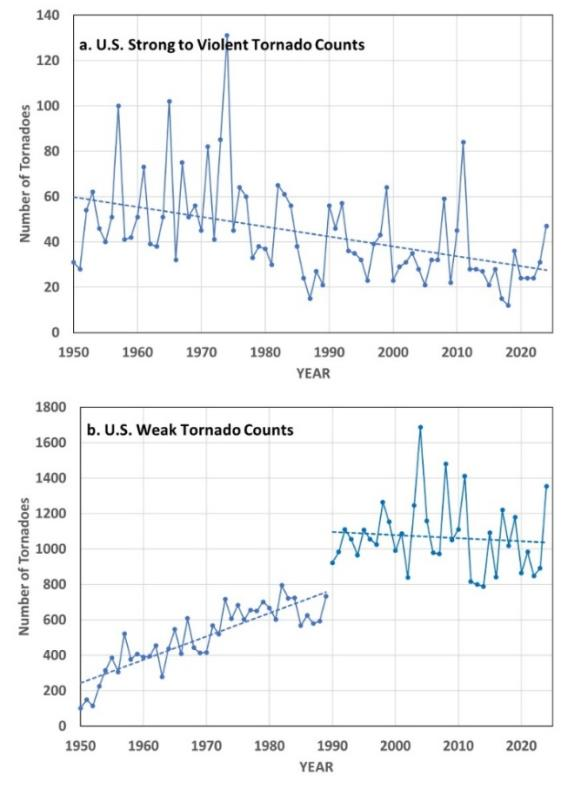
\includegraphics[width=0.9\textwidth]{bilder/bilderKlima-0060.jpg}\\[1cm]
\end{center}
\caption{Jährliche US-Tornado-Zahlen für (a) starke bis heftige Tornados (EF3 bis EF5) und (b) schwache Tornados (EF0 bis EF2). Basierend auf NOAA Storms Prediction Center Daten, verfügbar unter \url{https://www.spc.noaa.gov/wcm/data/1950-2024_actual_tornadoes.csv}}
\end{figure}

\section{Überschwemmung}
Veränderungen bei Überschwemmungen wurden wie folgt bewertet:
\begin{quote}
AR6: Der SREX \textbf{bewertete geringes Vertrauen für beobachtete Veränderungen in der Magnitude oder Häufigkeit von Überschwemmungen} auf globaler Ebene. Diese Bewertung wurde vom AR5-Bericht bestätigt. Der SR15 fand Zunahmen der Überschwemmungshäufigkeit und extremer Abflüsse in einigen Regionen, aber Abnahmen in anderen Regionen... Die hydrologische Literatur zu beobachteten Überschwemmungsveränderungen ist heterogen und konzentriert sich auf regionale und subregionale Beckenebenen, was es schwierig macht, sie auf globaler und manchmal regionaler Ebene zu synthetisieren. (Kapitel 11.5)
AR6: Die Saisonalität von Überschwemmungen hat sich in kalten Regionen verändert, wo Schneeschmelze das Abflussregime als Reaktion auf die Erwärmung dominiert (hohes Vertrauen). Das Vertrauen in Spitzenabflusstrends über vergangene Jahrzehnte auf globaler Ebene ist gering. (Kapitel 11.5)
NCA4: Trends bei extremen hohen Werten des Abflusses sind \textbf{gemischt} über die Vereinigten Staaten. Die Analyse von 200 US-Abflussmessern zeigt Gebiete sowohl zunehmender als auch abnehmender Überschwemmungsmagnitude, liefert aber \textbf{keine robusten Belege dafür}, dass diese Trends menschlichen Einflüssen zuzuschreiben sind (S. 240-241).
\end{quote}

Das Fehlen detektierbarer US-weiter Trends bei Überschwemmungen ist konsistent mit den Befunden in Abschnitt 6.4 über das Fehlen kohärenter Veränderungen bei extremen Niederschlägen.

\section{Dürren}
Bewertungen von Dürretrends waren wie folgt.

\begin{quote}
AR6: Wenige AR6-Regionen zeigen beobachtete Zunahmen meteorologischer Dürre (Abschnitt 11.9, S. 1575).

AR6: Zunehmende Trends bei landwirtschaftlichen und ökologischen Dürren wurden auf allen Kontinenten beobachtet (mittleres Vertrauen), aber Abnahmen nur in einer AR6-Region (mittleres Vertrauen). Zunehmende Trends bei hydrologischen Dürren wurden in wenigen AR6-Regionen beobachtet. (Kapitel 11 Zusammenfassung)

NCA4: Als Folge dieser erhöhten Niederschläge \textbf{sind die Dürrestatistiken über die gesamten CONUS zurückgegangen}. (S. 233)

NCA4: Jüngste Dürren und damit verbundene Hitzewellen haben in einigen Regionen der Vereinigten Staaten Rekordintensität erreicht; jedoch bleibt nach geografischem Maßstab und Dauer die Dust Bowl-Ära \textbf{der 1930er Jahre das Referenzdürre}- und extreme Hitzeereignis in der historischen Aufzeichnung (sehr hohes Vertrauen). (S. 231)

SREX: Aus einer paläoklimatischen Perspektive \textbf{sind jüngste Dürren nicht beispiellos}, mit schweren 'Megadürren', die in der paläoklimatischen Aufzeichnung für Europa, Nordamerika und Australien berichtet werden. (S. 170)
\end{quote}

\begin{figure}[H]
\begin{center}
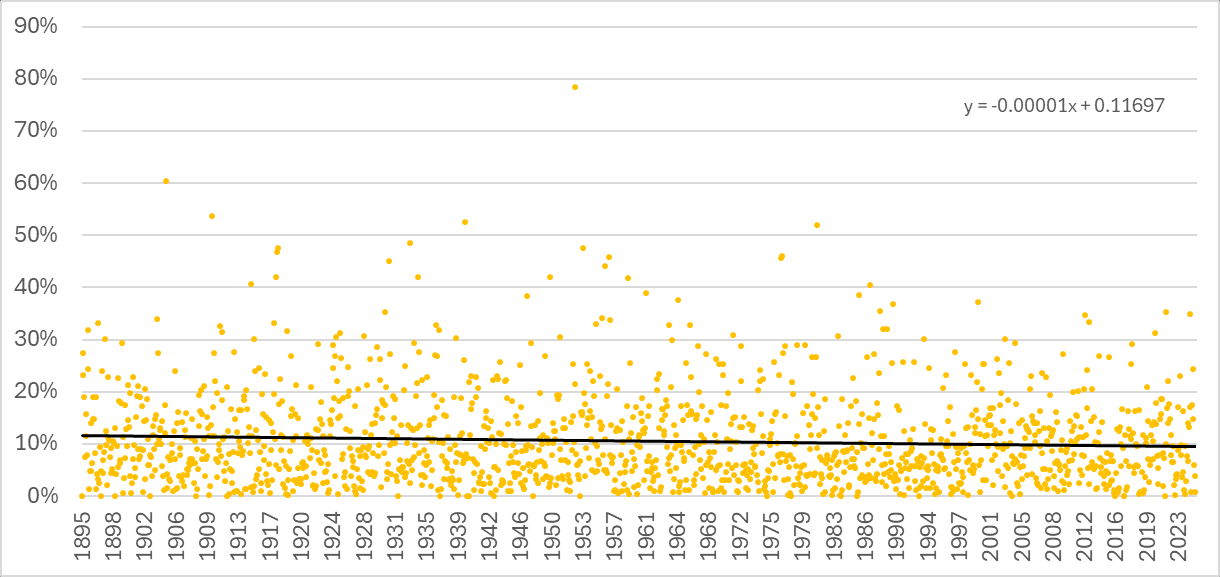
\includegraphics[width=0.9\textwidth]{bilder/bilderKlima-0061.png}\\[1cm]
\end{center}
\caption{Monatlicher Prozentsatz der USA, der als "Sehr Trocken" klassifiziert wird, 1895—2025. Datenquelle: NOAA https://www.ncei.noaa.gov/access/monitoring/uspa/wet-dry/0 Kleinste-Quadrate-Trendlinie hinzugefügt.}
\end{figure}

Wie in Abbildung 6.7.1 gezeigt, zeigen US-Langzeitdaten einen insignifikant rückläufigen Trend bei extremer Trockenheit (-0,001 Prozent pro Jahr).

Kogan et al. (2020) untersuchen ein 38-jähriges hochauflösendes satellitenbasiertes Dürremaß und schließen, dass sich die globale Dürre nicht intensiviert hat und nicht mit dem Klimawandel verbunden ist: \emph{Es ist möglich, fest zu stellen, dass die globalen und hauptgetreideländerspezifischen Dürregebiets- und Intensitätstrends nicht der globalen Klimaerwärmung seit den 1980er Jahren gefolgt sind.}

Zusammenfassend gibt es keine Evidenz für zunehmende meteorologische Dürrenhäufigkeit oder -intensität in den USA oder global über die jüngsten Jahrzehnte.

\section{Waldbrände}
Das IPCC hat keine Attributionsbewertung von Waldbränden bereitgestellt. Wie in Abbildung 6.8.1 gezeigt, zeigt die globale Waldbrand-Aktivität, gemessen von der European Space Agency, einen Abwärtstrend im 21. Jahrhundert.

\begin{figure}[H]
\begin{center}
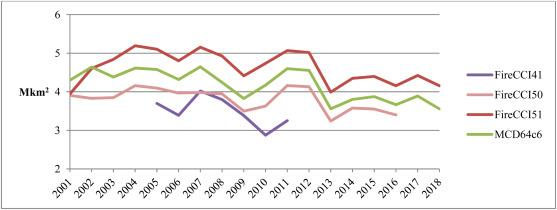
\includegraphics[width=0.9\textwidth]{bilder/bilderKlima-0063.jpg}\\[1cm]
\end{center}
\caption{Globale Waldbrandfläche 2001-2018. Quelle: Von Lizundia-Loiola et al. (2021) Abbildung 12. Die verschiedenfarbigen Linien repräsentieren Datenprodukte, die von verschiedenen Satelliten und Algorithmen abgeleitet wurden.}
\end{figure}

Globale Daten zeigen, dass die Waldbrandabdeckung auf jedem Kontinent konstant oder rückläufig ist (Samborska und Ritchie, 2024). Jedoch gibt es Evidenz, dass die Intensität von Bränden in einigen Regionen sich verschlechtert (Cunningham et al. 2024) und dass Waldbrände zu einem Nettoverlust der globalen Waldbedeckung über 2001-2019 führten (Tyukavina et al. 2022).

Aktive Feuerunterdrückung seit 1900 macht es schwierig, eine natürliche Grundlinie für Waldbrand-Aktivität in den USA zu etablieren. Paläoklimatische Evidenz zeigt, dass vergangene Aktivität viel höher war als heute. Marlon et al. (2012) verwendeten sedimentäre Kohleschichten, um die Feuergeschichte der westlichen USA für die letzten 1400 Jahre zu rekonstruieren und passten auch ein Modell an, um Feueraktivität als Funktion klimatischer Bedingungen vorherzusagen. Ihre Ergebnisse sind in Abbildung 6.8.2 unten zusammengefasst (von Abbildung 2 in ihrer Arbeit). Es gab ein wachsendes Waldbranddefizit über das 20. Jahrhundert. Mit anderen Worten, wie viel Feuer auch immer im 20. Jahrhundert beobachtet wurde, es war weniger als das, was in früheren Jahrhunderten basierend auf den klimatischen Bedingungen beobachtet worden wäre. Parks et al. (2025) finden ebenso, dass trotz der jüngsten Zunahme der Waldbrand-Brandfläche in Nordamerika ein erhebliches Waldbranddefizit relativ zu historischen Waldbrandregimen bestehen bleibt.

\begin{figure}[H]
\begin{center}
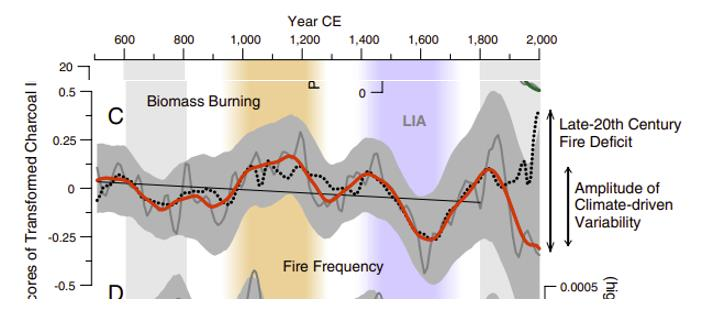
\includegraphics[width=0.9\textwidth]{bilder/bilderKlima-0064.jpg}\\[1cm]
\end{center}
\caption{Feuerhäufigkeit und Feuerdefizit in den USA. Die rote Linie zeigt die geglättete Kohleaufzeichnung und die schwarze gepunktete Linie zeigt die vorhergesagte Kohleaufzeichnung basierend auf klimatischen Bedingungen. Modell. Quelle: Marlon et al. (2012) Abbildung 2.}
\end{figure}

US-Daten des National Interagency Fire Centre (NIFC) von 1926 bis 2023 sind in Abbildung 6.8.3 gezeigt. Das NIFC hat die Daten vor 1960 von seiner aktuellen Website entfernt mit der Begründung, dass sich die Messmethoden nach 1960 änderten, wodurch der Vergleich unzuverlässig wird. Dennoch, nur auf das Intervall nach 1985 fokussierend, nimmt die Anzahl der Brände nicht zu. Die verbrannte Fläche nahm zu, aber nur bis etwa 2007.

Waldbrände waren schon immer ein Teil der Natur, und sie können sicherlich Bedingungen schaffen, die kurzfristig für alles Leben, einschließlich Menschen, unwirtlich sind. Die Wissenschaft hat den allgemeinen Nutzen und die Notwendigkeit von Waldbränden bestätigt. Während jüngste hochkarätige Brände und Saisons als Erinnerung an die potenzielle zerstörerische Auswirkung dienen, bleibt der hochkarätigste US-Waldbrand das 1910 Big Blowup-Feuer im US-Westen, das über drei Millionen Acres zerstörte und ganze Städte wie Taft, MT eliminierte (Apple, 2020). Das 1910-Feuer formte den US Forest Service um (National Forest Foundation 2022), was zu einem Fokus auf Feuerunterdrückung mit dem primären Ziel führte, alle Waldbrände zu besiegen (Forest History Society, 2022). Dies führte zur "10-Uhr-Regel" in 1935, die erforderte, dass alle an einem Tag entdeckten Brände bis 10 Uhr am folgenden Tag kontrolliert werden mussten (National Forest Foundation, 2022).

Während die Bekämpfung aller Brände ein edles Ziel schien, begannen Fragen darüber aufzukommen, ob dieses Verhalten "der Wissenschaft folgte" (U.S. Forest Service, 2022). Über die Zeit hat der US Forest Service begonnen, seine Ziele zu überdenken und zu erkennen, dass neue Ansätze wie verschriebene Brände, Brennstoffelimination und kontrollierte Waldbrände angemessener sind (Sommer, 2016). Jüngste Forschung validiert diesen Ansatz und erkennt, dass häufigere kleinere Brände wahrscheinlich zu gesünderen Wäldern, Wasserökosystemen und Biodiversität führen (Stephens et al., 2021).

\begin{figure}[H]
\begin{center}
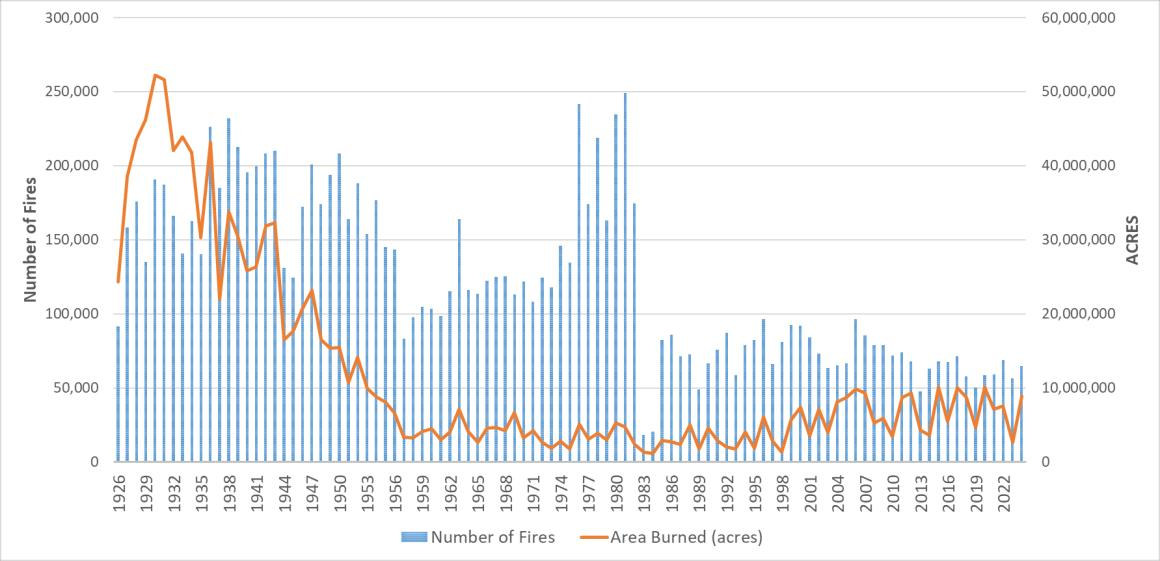
\includegraphics[width=0.9\textwidth]{bilder/bilderKlima-0065.jpg}\\[1cm]
\end{center}
\caption{US-Waldbrände 1926 bis 2023. Quelle: Nach 2018: National InterAgency Fire Center Daten https://www.nifc.gov/fire-information/statistics/wildfires. Vor 2017 webarchive.org (n.d.).}
\end{figure}

\vfill
\noindent\textbf{Literaturverzeichnis:}

\begingroup
\parindent=0pt
\everypar{\hangindent=2em\hangafter=1\relax}

Apple, C. (2020, January 21). 1910 fire – The big burn across Montana and Idaho. The Spokesman-
Review. https://www.spokesman.com/stories/2020/jan/19/1910-fire-big-burn-across-montana-and-
idaho/

Bell, Gerald D. and Muthuvel Chelliah, “Leading Tropical Modes Associated with Interannual and
Multidecadal Fluctuations in North Atlantic Hurricane Activity,” Journal of Climate 19, no. 4
(February 15, 2006): 590–612, https://doi.org/10.1175/JCLI3659.1.

Brewer, W. H. (1930). Up and down California in 1860–1864: The journal of William H. Brewer.
University of California Press.

Christy, J. R., Norris, W. B., and McNider, R. T. (2009). Surface temperature variations in East Africa
and possible causes. Journal of Climate, 22(12), 3342–3356. https://doi.org/10.1175/2008JCLI2726.1

Cohn, T. A. and Lins, H. F. (2005). Nature’s style: Naturally trendy. Geophysical Research Letters,
32(23). https://doi.org/10.1029/2005GL024476

Colorado State University. (2025). Realtime tropical cyclone guidance.
\url{https://tropical.atmos.colostate.edu/Realtime/index.php}

Cunningham, C.X., G.J. Williamson, and D. Bowman (2024) Increasing frequency and intensity of the
most extreme wildfires on Earth. Nature Ecology and Evolution 8, 1420–1425.
https://doi.org/10.1038/s41559-024-02452-2

Forest History Society (2022). The 1910 fires. https://foresthistory.org/research-explore/us-forest-service-
history/policy-and-law/fire-u-s-forest-service/famous-fires/the-1910-fires/

Gershunov, A., and K. Guirguis (2012). California heat waves in the present and future. Geophysical
Research Letters, 39(18). https://doi.org/10.1029/2012GL052979

Gershunov, A., T. Shulgina, F.M. Ralph, D.A. Lavers J.J. and Rutz (2017). Assessing the climate-scale
variability of atmospheric rivers affecting western North America. Geophysical Research Letters,
44(15), 7900–7908. https://doi.org/10.1002/2017GL074175

Goldenberg, Stanley et al., “The Recent Increase in Atlantic Hurricane Activity: Causes and
Implications,” Science 293, no. 5529 (July 20, 2001): 474–479,
\url{https://doi.org/10.1126/science.1060040.}

Howarth, M. E., C.D. Thorncroft, and L.F. Bosart (2019). Changes in extreme precipitation in the
Northeast United States: 1979–2014. Journal of Hydrometeorology, 20(4), 673–689.
https://doi.org/10.1175/JHM-D-18-0155.1

Hurst, H. E. (1951). Long term storage capacities of reservoirs. Transactions of the American Society of
Civil Engineers, 116, 776–808.

Intergovernmental Panel on Climate Change (IPCC). (2021). Climate change 2021: The physical science
basis. Contribution of Working Group I to the Sixth Assessment Report of the Intergovernmental
Panel on Climate Change (V. Masson-Delmotte et al., Eds.). Cambridge University Press.
https://www.ipcc.ch/report/ar6/wg1/

Jong, B.-T., H. Murakami, T.L. Delworth and W.F. Cooke (2024). Contributions of tropical cyclones and
atmospheric rivers to extreme precipitation trends over the Northeast US. Earth’s Future, 12,
e2023EF004370. https://doi.org/10.1029/2023EF004370

Karl, T.R., H.F. Diaz, and G. Kukla. (1988): Urbanization: Its detection and effect on the United States
climate record. Journal of Climate, 1, 1099-1123
\url{https://journals.ametsoc.org/view/journals/clim/1/11/1520-
0442_1988_001_1099_uidaei_2_0_co_2.xml}

Karl, T. R., C.N. Williams Jr., F.T. Quinlan, and T.A. Boden (1990). United States Historical
Climatology Network (HCN) serial temperature and precipitation data (Publication No. 3404). Oak
Ridge National Laboratory.

Klotzbach, Phil et al. (2018) Continental U.S. Hurricane Landfall Frequency and Associated Damage:
Observations and Future Risks, Bulletin of the American Meteorological Society 99, no. 7 (July
2018): 1359–1376, https://doi.org/10.1175/BAMS-D-17-0184.1.

Kogan, Feliz, Wei Guob and Wenze Yang (2020) “Near 40-year drought trend during 1981-2019 earth
warming and food security” Geomatics, Natural Hazards and Risk Vol 11(1)

Koutsoyiannis, D. (2013) Hydrology and Change. Hydrological Sciences Journal 58(6)
http://dx.doi.org/10.1080/02626667.2013.804626

Lizundia-Loiola, J., et al. (2020) A spatio-temporal active-fire clustering approach for global burned area
mapping at 250 m from MODIS data. Remote Sensing of the Environment 236, 111493,
https://doi.org/10.1016/j.rse.2019.111493

Markonis, Y., and D. Koutsoyiannis (2016). Scale-dependence of persistence in precipitation records.
Nature Climate Change, 6, 399–401. https://doi.org/10.1038/nclimate2894

Marlon, Jennifer, Patrick J Bartlein, Daniel G. Gavin et al. (2012) Long-term perspective on wildfires in
the western USA Proceedings of the National Academy of Sciences February 14 2012
https://www.pnas.org/doi/pdf/10.1073/pnas.1112839109

Maue, R. N. (2025). Climatlas: Tropical cyclones. https://climatlas.com/tropical/

Maue, R. N. (2011) Recent historically low tropical cyclone activity. Geophysical Research Letters 38,
L14803, doi:10.1029/2011GL047711

McKitrick, R., and J.R. Christy (2019). Assessing changes in US regional precipitation on multiple time
scales. Journal of Hydrology, 578, 124074. \url{https://doi.org/10.1016/j.jhydrol.2019.124074}

McKitrick, R. and J.R. Christy (2025), “Data and Code for CWG2025 Report”, Mendeley Data, V1, doi:
10.17632/by76s7rxfb.1

McNider, R.T., G.J. Steeneveld, A.A.M. Holtslag, R.A. Pielke Sr., S. Mackaro, A. Pour-Biazar, J.
Walters, U. Nair, and J.R. Christy, 2012: Response and sensitivity of the nocturnal boundary layer
over land to added longwave radiative forcing. Journal of Geophysical Research., 117, D14106,
doi:10.1029/2012JD017578.

Null, J. and J. Hulbert, “California Washed Away: The Great Flood of 1862,” Weatherwise 60, no. 1
(2007): 26–30, https://doi.org/10.3200/wewi.60.1.26-30

National Forest Foundation. (2022). Blazing battles: The 1910 fire and its legacy.
\url{https://www.nationalforests.org/our-forests/your-national-forests-magazine/blazing-battles-the-1910-
fire-and-its-legacy}

National Interagency Fire Center. (2024). Wildfire statistics. https://www.nifc.gov/fire-
information/statistics/wildfires

NCA4. (2017). Climate science special report: Fourth National Climate Assessment, Volume I (D. J.
Wuebbles, D. W. Fahey, and K. A. Hibbard, Eds.). U.S. Global Change Research Program.
https://doi.org/10.7930/J0J964J6

NCA5. (2023). Fifth National Climate Assessment (A. R. Crimmins et al., Eds.). U.S. Global Change
Research Program. https://doi.org/10.7930/NCA5.2023.CH1 (accessed May 22, 2025)

NOAA Hurricane Research Division. (2025a). All U.S. hurricanes (1851–2019).
\url{https://www.aoml.noaa.gov/hrd/hurdat/All_U.S._Hurricanes.html}

NOAA Hurricane Research Division. (2025b). Most intense (3, 4, 5) continental United States
hurricanes: 1851–1970, and 1983–2023. \url{https://www.aoml.noaa.gov/hrd/hurdat/most_intense.html}

Overland, J. E. (2021). Causes of the record-breaking Pacific Northwest heatwave, late June 2021.
Atmosphere, 12(11), 1434. https://doi.org/10.3390/atmos12111434

Pan, M., M. Lu and U. Lall (2024). Diversity of cross-Pacific atmospheric river main routes.
Communications Earth and Environment, 5, 378. https://www.nature.com/articles/s43247-024-
01552-y

Parks, Sean, Christopher Guiterman, Ellis Margolis et al. (2025) A fire deficit persists across diverse
North American forests despite recent increases in area burned. Nature Communications 16
\url{https://www.nature.com/articles/s41467-025-56333-8}

Pielke, R. A., et al. (2011). Land use/land cover changes and climate: Modeling analysis and
observational evidence. Wiley Interdisciplinary Reviews: Climate Change, 2, 828–850.
https://doi.org/10.1002/wcc.144

Porter, K., et al. (2011). Overview of the ARkStorm scenario. U.S. Geological Survey.

Quinlan, F. T., T. R. Karl, and C.N. Williams Jr. (1987). United States Historical Climatology Network
(USHCN) serial temperature and precipitation data (NDP-019). Oak Ridge National Laboratory.

Runnalls, K.E. and T.R. Oke, 2006: Technique to detect microclimate inhomogeneities in historical
records of screen-level air temperature. Journal of Climate, 19, 959-978.
\url{https://doi.org/10.1175/JCLI3663.1}

Samborska, V., and H. Ritchie (2024). Wildfires. Our World in Data. \url{https://ourworldindata.org/wildfires}

Seneviratne, S. et al. (2021) “Chapter 11: Weather and Climate Extreme Events in a Changing Climate.”
In Climate Change 2021: The Physical Science Basis. Contribution of Working Group I to the Sixth
Assessment Report of the Intergovernmental Panel on Climate Change, edited by V. Masson-
Delmotte, P. Zhai, A. Pirani, S.L. Connors, C. Péan, S. Berger, N. Caud, et al., 1513–1766.
Cambridge: Cambridge University Press, 2021. https://doi.org/10.1017/9781009157896.013.

Sommer, L. (2016, November 7). Let it burn: The Forest Service wants to stop putting out some fires.
KQED. https://www.kqed.org/science/1134217/let-it-burn-the-forest-service-wants-to-stop-putting-
out-some-fires

Stephens, Scott et al., (2021) “Fire, Water, and Biodiversity in the Sierra Nevada: A Possible Triple Win,”
Environmental Research Communications 3, no. 8 (August 6, 2021): p. 081004,
https://doi.org/10.1088/2515-7620/ac17e2.

Tyukavina Alexandra , Peter Potapov, Matthew Hansen et al. (2022) Global Trends of Forest Loss Due to
Fire From 2001 to 2019, Frontiers in Remote Sensing. Volume 3
\url{https://www.frontiersin.org/journals/remote-sensing/articles/10.3389/frsen.2022.825190/full}

U.S. Forest Service. (2022). Managing fire. https://www.fs.usda.gov/science-technology/fire

USGCRP. (2023). USGCRP indicators platform: Heat waves.
\url{https://www.globalchange.gov/indicators/heat-waves}

Vecchi, Gabriel A. and Thomas R. Knutson (2011) “Estimating Annual Numbers of Atlantic Hurricanes
Missing from the HURDAT Database (1878–1965) Using Ship Track Density,” Journal of Climate
24, no. 6 (2011): 1736–1746, https://doi.org/10.1175/2010JCLI3810.1.

Villarini, Gabriele, Gabriel A. Vecchi, and James A. Smith, “U.S. Landfalling and North Atlantic
Hurricanes: Statistical Modeling of Their Frequencies and Ratios,” Monthly Weather Review 140, no.
1 (January 2012): 44–65, https://doi.org/10.1175/MWR-D-11-00063.1.

Web Archive. (n.d.). Archive of NIFC fire data.
\url{https://web.archive.org/web/20200212033452/https://www.nifc.gov/fireInfo/fireInfo_stats_totalFires.
html}

Yang, L., Y. Yang, Y. Shen, et al. (2024). Urban development pattern’s influence on extreme rainfall
occurrences. Nature Communications, 15, 3997. https://doi.org/10.1038/s41467-024-48533-5

Zhang, W., G. Villarini, G.A. Vecchi, and J.A. Smith, J. A. (2018). Urbanization exacerbated the rainfall
and flooding caused by Hurricane Harvey in Houston. Nature, 563, 384–388.
https://doi.org/10.1038/s41586-018-0676-z
\endgroup


\cleardoublepage
\FigureNumbersByChapter 
\chapter{VERÄNDERUNGEN DES MEERESSPIEGELS}
\paragraph{Kapitelzusammenfassung}
\begin{quote}
Seit 1900 ist der globale durchschnittliche Meeresspiegel um etwa 8 Zoll gestiegen. Meeresspiegeländerungen entlang der US-Küsten sind sehr variabel und stehen in Verbindung mit lokalen Variationen in Prozessen, die zum Absinken beitragen, sowie mit Meeresströmungsmustern. Die größten Meeresspiegelanstiege entlang der US-Küsten sind in den Regionen Galveston, New Orleans und der Chesapeake Bay - jeder dieser Orte ist mit erheblichem lokalem Landabsinken (Subsidenz) verbunden, das nicht mit dem Klimawandel zusammenhängt.

Extreme Projektionen des globalen Meeresspiegelanstiegs sind mit einem unplausiblen extremen Emissionsszenario und der Einbeziehung schlecht verstandener Prozesse verbunden, die mit hypothetischen Eisschild-Instabilitäten zusammenhängen. Bei der Bewertung der AR6-Projektionen bis 2050 (mit Bezug auf die Referenzperiode 1995-2014) ist bis 2025 fast die Hälfte des Intervalls verstrichen, wobei der Meeresspiegel langsamer ansteigt als vorhergesagt. US-Pegelmessungen zeigen keine offensichtliche Beschleunigung über die historische durchschnittliche Rate des Meeresspiegelanstiegs hinaus.
\end{quote}

\section{Globaler Meeresspiegelanstieg}
Der globale Meeresspiegelanstieg ist wohl der wichtigste klimatische Wirkungsfaktor, der eindeutig mit steigenden Temperaturen verbunden ist. Auf globaler Ebene erhöht die Erwärmung den Meeresspiegel durch thermische Expansion des Meerwassers und durch das Schmelzen von Gletschern und Eisschilden. Variationen in der Landwasserspeicherung sind ein weiterer wichtiger Faktor. Auf regionaler Ebene wird die Meeresspiegeländerung von großräumigen Meeresströmungsmustern und geologischen Prozessen und Verformungen durch die Umverteilung von Eis und Wasser beeinflusst. Lokal sind auch vertikale Landbewegungen durch geologische Prozesse, Grundwasserentnahme und Förderung fossiler Brennstoffe wichtig.

AR6 schätzt, dass der globale mittlere Meeresspiegel zwischen 1901 und 2018 um 7,9 (5,9–9,8) Zoll gestiegen ist, wobei sich die Rate des Meeresspiegelanstiegs in den letzten Jahrzehnten beschleunigt hat. Auf der Ebene der Ozeanbecken sind die Meeresspiegel im Zeitraum 1993–2018 am schnellsten im Westpazifik und am langsamsten im Ostpazifik gestiegen (Fox-Kemper et al., 2021). Die Rate des globalen Meeresspiegelanstiegs wird auf 0,12 Zoll/Jahr geschätzt, etwa die Höhe von zwei übereinander gestapelten Pfennigen (NASA, 2020).

Die Beobachtungssysteme für den globalen Meeresspiegelanstieg haben sich im Satellitenzeitalter erheblich verbessert, insbesondere mit dem Aufkommen von Satellitenaltimetern im Jahr 1993. Lokale Pegel haben für das vergangene Jahrhundert nützliche Daten geliefert, und für einige wenige Orte sogar noch länger. Nach dem Ende der Kleinen Eiszeit Mitte des neunzehnten Jahrhunderts zeigen Pegel, dass der globale mittlere Meeresspiegel während der Periode 1820–1860 zu steigen begann, deutlich vor den meisten anthropogenen Treibhausgasemissionen.

\section{US-Meeresspiegelanstieg}
Beobachtete und vorhergesagte Raten des mittleren globalen Meeresspiegelanstiegs könnten aufgrund lokaler Prozesse für spezifische Standorte wenig wissenschaftliche Relevanz haben (NOAA, 2025). Abbildung 7.1 zeigt, dass in Kanada und Alaska (und auch im nördlichen Washington) der Meeresspiegel sinkt, aufgrund von Anhebung durch glaziale Erholung. Die meisten Pegel an der Pazifikküste zeigen niedrige Raten des Meeresspiegelanstiegs, während die größten US-Raten an der Golfküste (Louisiana und Texas) und in den mittelatlantischen Staaten (Chesapeake Bay-Region) auftreten.

\begin{figure}[H]
\begin{center}
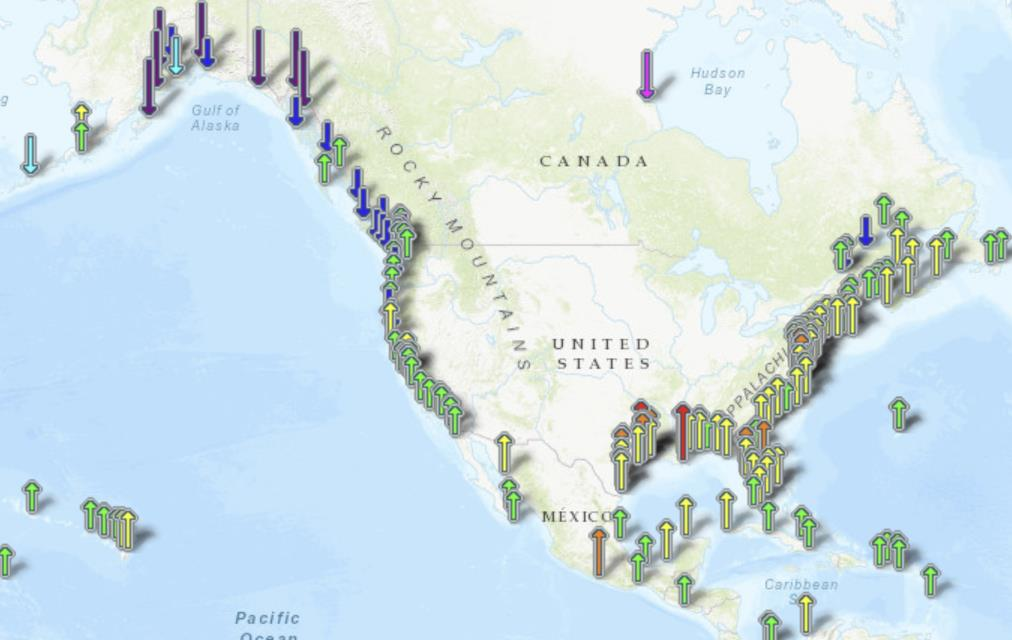
\includegraphics[width=0.9\textwidth]{bilder/bilderKlima-0067.jpg}\\[1cm]
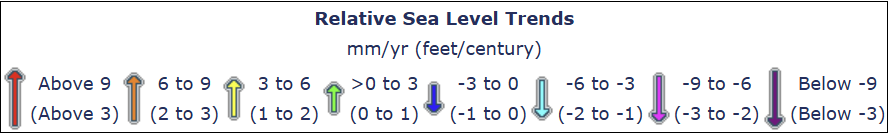
\includegraphics[width=0.9\textwidth]{bilder/bilderKlima-0068.png}\\[1cm]
\end{center}
\caption{Karte der Raten des relativen Meeresspiegelanstiegs entlang der US-Küste (NOAA, https://tidesandcurrents.noaa.gov/sltrends/). Zum Vergleich: 3 mm = 0,12 Zoll.}
\end{figure}

Messungen des relativen Meeresspiegelanstiegs durch Pegel vermischen die klimatologisch relevante Zunahme des Meerwasservolumens mit lokalen vertikalen Landbewegungen. Letztere, die von Ort zu Ort variieren, werden am besten mit einer Global Positioning System (GPS)-Station gemessen, die sich nahe dem Pegel befindet. Sie werden von einer Reihe von Prozessen angetrieben, die mit dem Klimasignal vergleichbar sein können und lokal das Risiko des Meeresspiegelanstiegs verschärfen (Subsidenz/Absinken) oder mildern (Anhebung) können (Wöppelmann und Marcos, 2016). Menschliche Aktivitäten, die Subsidenz auslösen, sind oft bedeutsam. Dazu gehören Bodenentwässerung (z.B. für städtische Entwicklung) und unterirdische Entnahme von Grundwasser oder Kohlenwasserstoffen.

Tabelle 7.1 zeigt den absoluten Meeresspiegelanstieg (ASLR) für ausgewählte Standorte, bestimmt aus der Summe des unkorrigierten relativen Meeresspiegelanstiegs (RSLR), wie er aus Pegelzeitreihen geschätzt wurde (NOAA, 2025), und den Messungen der vertikalen Landbewegung (VLM) (NAS, 2012; Letetrel et al., 2015; Karegar et al., 2016). Der absolute Meeresspiegelanstieg für jeden dieser Standorte ist aufgrund lokaler Subsidenz erheblich kleiner als der gemessene relative Meeresspiegelanstieg. Mehr als die Hälfte des gemessenen relativen Meeresspiegelanstiegs wird dem Landabsinken zugeschrieben für diese Standorte: San Francisco, Galveston, Grand Isle. Zum Vergleich wird die globale durchschnittliche Rate des absoluten Meeresspiegelanstiegs auf 0,12 Zoll/Jahr geschätzt.

%%Tabelle

StandortRSLRVLMASLRSan Francisco, CA+0,08-0,06+0,02Galveston, TX+0,26-0,19+0,07Grand Isle, LA+0,36-0,28+0,08St Petersburg, FL+0,12-0,02+0,10New York City, NY+0,11-0,05+0,06
Tabelle 7.1 Absoluter Meeresspiegelanstieg (Zoll/Jahr) bestehend aus relativem Meeresspiegelanstieg (RSLR) plus vertikaler Landbewegung (VLM)


\subsection{San Francisco Bay}
In den vergangenen 100 Jahren ist der relative Meeresspiegel in der San Francisco Bay-Region um 7,8 Zoll gestiegen, mit einer durchschnittlichen Rate von 0,08 Zoll/Jahr (Abbildung 7.2). Wie in Tabelle 7.1 gezeigt, beträgt San Franciscos vertikale Landbewegung -0,06 Zoll/Jahr (Absinken), was eine jüngste absolute Rate von +0,02 Zoll/Jahr ergibt. Teile von Treasure Island, San Francisco International Airport und Foster City sinken um bis zu 0,4 Zoll/Jahr (Shirzaei und Bürgmann, 2018). Probleme in der San Francisco Bay-Region, einschließlich Bedrohungen für den Flughafen, werden hauptsächlich durch Bodenverdichtung in Aufschüttungszonen verursacht, die früher Feuchtgebiete waren, nicht durch das langsame Kriechen des globalen Meeresspiegelanstiegs.

\begin{figure}[H]
\begin{center}
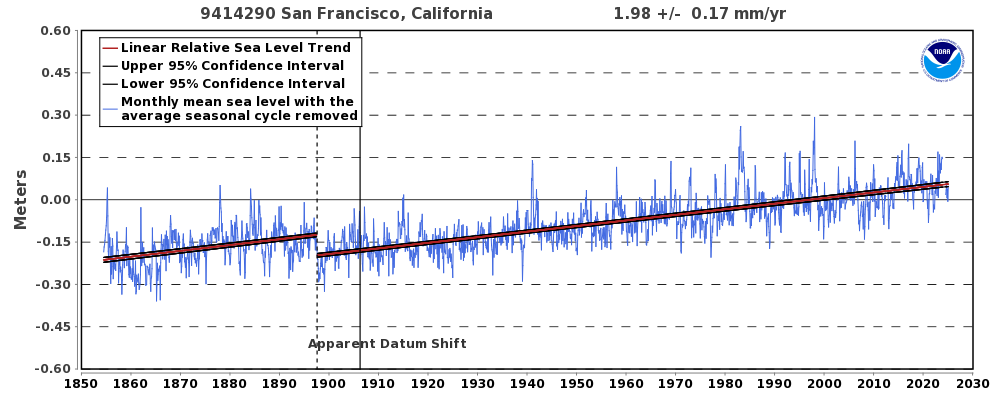
\includegraphics[width=0.9\textwidth]{bilder/bilderKlima-0069.png}\\[1cm]
\end{center}
\caption{Pegelmessungen in San Francisco, Kalifornien, erhalten von NOAA - \url{https://tidesandcurrents.noaa.gov/sltrends/sltrends_station.shtml?id=9414290} (heruntergeladen 4/22/25).}
\end{figure}

\subsection{Galveston - Houston}
Langzeitmessungen des Pegels am Galveston Pier 21 zeigen einen Meeresspiegelanstieg von 2,18 Fuß im vergangenen Jahrhundert oder eine Rate von 0,26 Zoll/Jahr (Abbildung 7.3). Die vertikale Landbewegung (Subsidenz) in Galveston wird auf -0,19 Zoll/Jahr geschätzt, was eine absolute Anstiegsrate von +0,07 Zoll/Jahr ergibt (Tabelle 7.1). Der U.S. Geological Survey fand heraus, dass der größte Teil der Oberflächensubsidenz in der Houston-Galveston-Region ein direktes Ergebnis von Grundwasserentnahmen ist (Kasmarek und Ramage 2017), die eine Verdichtung der Aquifer-Sedimente verursachten, hauptsächlich in den feinkörnigen Schluff- und Tonschichten. Bis 1979 war in Houston eine Subsidenz von bis zu 10 Fuß aufgetreten.

\begin{figure}[H]
\begin{center}
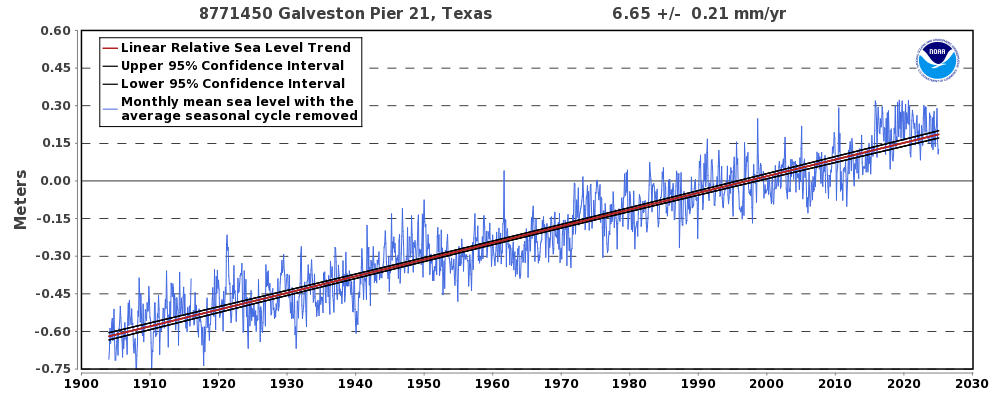
\includegraphics[width=0.9\textwidth]{bilder/bilderKlima-0070.png}\\[1cm]
\end{center}
\caption{Pegelmessungen Galveston Pier, TX, erhalten von NOAA - \url{https://tidesandcurrents.noaa.gov/sltrends/sltrends_station.shtml?id=8771450} (heruntergeladen 4/22/2025).}
\end{figure}

\subsection{New Orleans und das Mississippi-Delta}
Langzeitmessungen des Pegels in Grand Isle, Louisiana, zeigen, dass der Meeresspiegel in den letzten 100 Jahren um etwas mehr als 3 Fuß gestiegen ist, mit einer durchschnittlichen Rate von 0,36 Zoll/Jahr (Abbildung 7.4).
Die vertikale Landbewegung (Subsidenz) wird auf -0,28 Zoll/Jahr geschätzt. Tabelle 7.1 gibt den absoluten Meeresspiegelanstieg mit +0,08 Zoll/Jahr an.

\begin{figure}[H]
\begin{center}
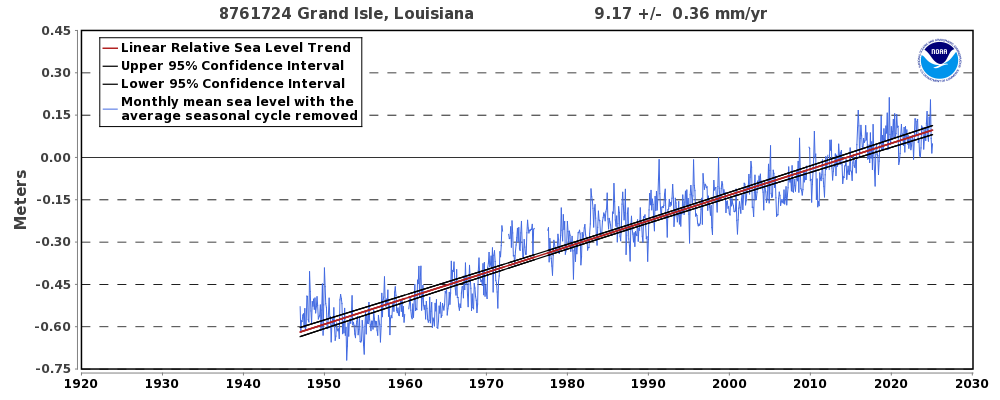
\includegraphics[width=0.9\textwidth]{bilder/bilderKlima-0071.png}\\[1cm]
\end{center}
\caption{Pegelmessungen in Grand Isle, LA, erhalten von NOAA - \url{https://tidesandcurrents.noaa.gov/sltrends/sltrends_station.shtml?id=8761724} (heruntergeladen 4/22/25).}
\end{figure}

Die Probleme des Meeresspiegelanstiegs und Landverlusts in der Mississippi-Delta-Region sind komplex, wobei geologische Subsidenz und der Rückgang der vom Mississippi River transportierten Sedimente die dominierenden Treiber sind. Der Bau von Dämmen im Einzugsgebiet seit den 1950er Jahren hat die Schwebstoff-Fracht des Mississippi um ~50 Prozent verringert (Maloney 2018). Eine neue Subsidenzkarte des Küstengebiets von Louisiana zeigt, dass die Küstenregion um etwa ein Drittel Zoll pro Jahr absinkt (Neinhuis et al. 2017), verbunden mit Grundwasser- und Ressourcenentnahme. Da die Höhenlage der Stadt im Durchschnitt ein bis zwei Fuß unter dem Meeresspiegel liegt, ist der Meeresspiegelanstieg durch anthropogene Erwärmung kaum der dominierende Treiber von New Orleans' Problemen.

\subsection{New York City}
New York City ist besonders verwundbar gegenüber den Auswirkungen des Meeresspiegelanstiegs, weil es hauptsächlich auf Inseln gebaut ist und 520 Meilen Küstenlinie hat. Messungen durch einen Pegel an der Südspitze von Manhattan (The Battery) zeigen, dass der relative Meeresspiegel in den vergangenen Jahrhundert um über 11 Zoll gestiegen ist, mit einer durchschnittlichen Rate von 0,11 Zoll/Jahr (Abbildung 7.5). Aber die vertikale Landbewegung in der New York City-Region beträgt -0,05 Zoll/Jahr (ungefähr 5 Zoll pro Jahrhundert), so dass die absolute Rate des Meeresspiegelanstiegs am Battery 0,06 Zoll/Jahr beträgt, oder etwa 55 Prozent des gemessenen relativen Meeresspiegelanstiegs.

\begin{figure}[H]
\begin{center}
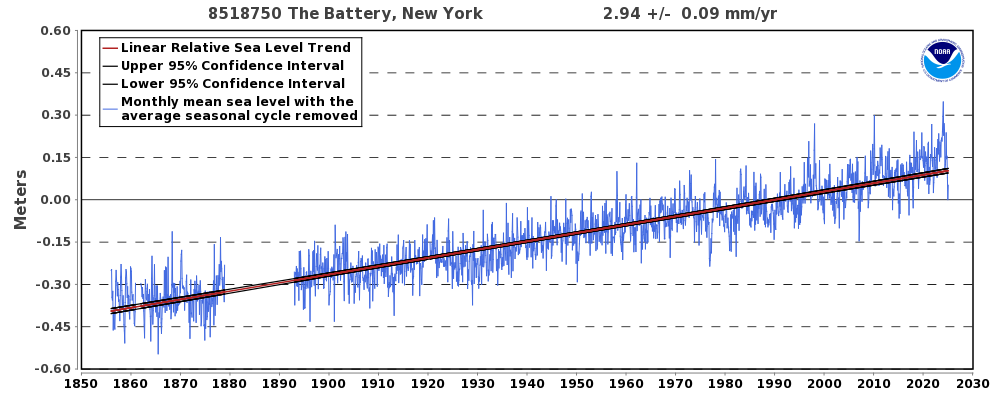
\includegraphics[width=0.9\textwidth]{bilder/bilderKlima-0072.png}\\[1cm]
\end{center}
\caption{Pegelmessungen am Battery, New York, erhalten von NOAA - \url{https://tidesandcurrents.noaa.gov/sltrends/sltrends_station.shtml?id=8518750} (heruntergeladen 4/22/25).}
\end{figure}

\section{Projizierter Meeresspiegelanstieg}
Die Besorgnis über den Meeresspiegelanstieg betrifft nicht die etwa acht Zoll globalen Anstiegs seit 1900. Vielmehr geht es um Projektionen eines beschleunigten Anstiegs basierend auf Simulationen eines sich erwärmenden Klimas durch das 21. Jahrhundert.

AR6 findet hohe Übereinstimmung zwischen veröffentlichten globalen mittleren Meeresspiegelprojektionen für 2050 mit geringer Sensitivität gegenüber Emissionsszenarien. Unter Berücksichtigung nur der Projektionen, die Eisschild-Prozesse einbeziehen, in deren Quantifizierung es mindestens mittleres Vertrauen gibt, fallen die globalen Meeresspiegelprojektionen für 2050 über alle Emissionsszenarien zwischen 3,94 und 15,75 Zoll (5.–95. Perzentil sehr wahrscheinlicher Bereich) relativ zur Referenzperiode 1995–2014 (Fox-Kemper et al., 2021).

Umgekehrt stellt AR6 fest, dass es geringe Übereinstimmung zwischen veröffentlichten globalen mittleren Meeresspiegelprojektionen für 2100 gibt, insbesondere für höhere Emissionsszenarien. Unter Berücksichtigung nur der Projektionen, die Eisschild-Prozesse darstellen, in deren Quantifizierung es mindestens mittleres Vertrauen gibt, liegen die AR6 globalen mittleren Meeresspiegelprojektionen für 2100 zwischen 7,9 und 39,4 Zoll (5.–95. Perzentil sehr wahrscheinlicher Bereich) unter dem mittleren Emissionsszenario SSP2–4.5 (Fox-Kemper et al., 2021). Es besteht tiefe Ungewissheit bezüglich der Projektionen des Meeresspiegelanstiegs bis 2100 aufgrund von Ungewissheiten in Eisschild-Instabilitäten, insbesondere für die höheren Emissionsszenarien.

Im Februar 2022 gab NOAA seine Projektionen des Meeresspiegelanstiegs für verschiedene Standorte entlang der US-Küste heraus (Sweet et al., 2022). Sie behaupten, dass bis 2050 der Meeresspiegel um einen Fuß am Battery in Manhattan gestiegen sein wird (relativ zu 2020). Ein Ein-Fuß-Anstieg in dreißig Jahren wäre mehr als doppelt so hoch wie die aktuelle Rate und etwa dreimal so hoch wie die durchschnittliche Rate über das vergangene Jahrhundert. In diesem historischen Kontext ist NOAAs Projektion bemerkenswert – wie in Abbildung 7.6 gezeigt, würde sie eine dramatische Beschleunigung über alles hinaus erfordern, was seit dem frühen 20. Jahrhundert beobachtet wurde. Aber noch bemerkenswerter ist, dass Sweet et al. (2022) sagen, dass dieser Anstieg „feststeht" – er wird unabhängig davon geschehen, was zukünftige Emissionen sind. Wir sollten in etwa einem Jahrzehnt wissen, ob diese Vorhersage Bestand hat.

\begin{figure}[H]
\begin{center}
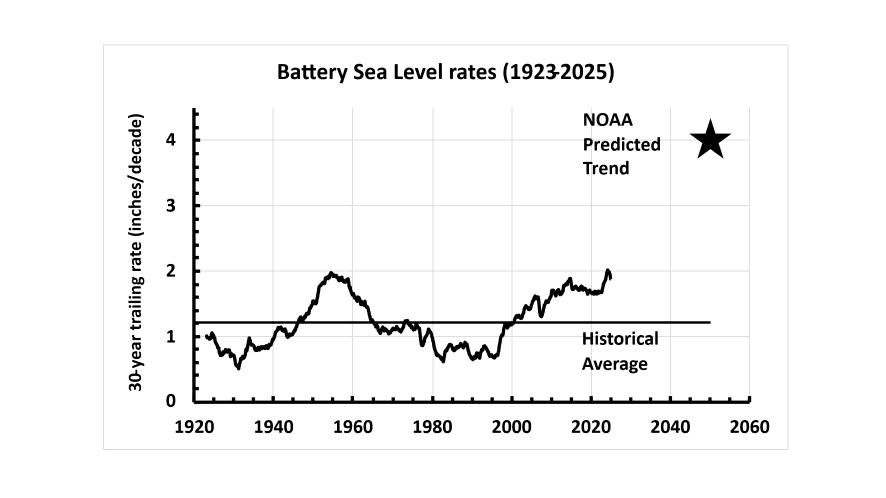
\includegraphics[width=0.9\textwidth]{bilder/bilderKlima-0073.png}\\[1cm]
\end{center}
\caption{Rate des Meeresspiegelanstiegs am Battery in Manhattan. Gezeigt ist der historische dreißigjährige nachlaufende Trend zusammen mit dem angeblich „feststehenden" NOAA-vorhergesagten Trend für 2050. Historische Daten: NOAA Tides and Current.}
\end{figure}

\vfill
\noindent\textbf{Literaturverzeichnis:}

\begingroup
\parindent=0pt
\everypar{\hangindent=2em\hangafter=1\relax}

Fox-Kemper, B., Hewitt, H. T., Xiao, C., Adalgeirsdóttir, G., Drijfhout, S. S., Edwards, T. L., ... \& Yu, Y.
(2021). Ocean, cryosphere and sea level change. In Climate Change 2021: The Physical Science
Basis. Contribution of Working Group I to the Sixth Assessment Report of the Intergovernmental
Panel on Climate Change (pp. 1211–1362). Geneva, Switzerland: Intergovernmental Panel on
Climate Change.

Karegar, M. A., Dixon, T. H., \& Engelhart, S. E. (2016). Subsidence along the Atlantic Coast of North
America: Insights from GPS and late Holocene relative sea level data. Geophysical Research Letters,
43(7), 3126–3133. https://doi.org/10.1002/2016GL068015
80

Kasmarek, M. C., \& Ramage, J. K. (2017). Water-level altitudes 2017 and water-level changes in the
Chicot, Evangeline, and Jasper aquifers and compaction 1973–2016 in the Chicot and Evangeline
aquifers, Houston-Galveston Region, Texas (Scientific Investigations Report 2017–5080). U.S.
Geological Survey. https://doi.org/10.3133/sir20175080

Letetrel, C., Becker, M., Llovel, W., \& Cazenave, A. (2015). Estimation of vertical land movement rates
along the coasts of the Gulf of Mexico over the past decades. Continental Shelf Research, 111(Part
A), 42–51. https://doi.org/10.1016/j.csr.2015.10.018

Maloney, J. M., Bentley, S. J., Xu, K., Obelcz, J., Georgiou, I. Y., \& Miner, M. D. (2018). Mississippi
River subaqueous delta is entering a stage of retrogradation. Marine Geology, 400, 12–23.
https://doi.org/10.1016/j.margeo.2018.03.001

National Academy of Science (NAS, 2012). Sea-level rise for the coasts of California, Oregon and
Washington: Past, present, and future. Appendix A: Vertical land motion and sea-level data along the
West Coast of the United States. National Academies Press.
https://nap.nationalacademies.org/catalog/13389/sea-level-rise-for-the-coasts-of-california-oregon-
and-washington

NASA. (2020). NASA sea level rise portal: 2020 edition. https://www.nasa.gov/specials/sea-level-rise-
2020/

National Oceanic and Atmospheric Administration (NOAA) Center for Operational Oceanographic
Products and Services. (n.d.). Sea level trends. https://tidesandcurrents.noaa.gov/sltrends/

NOAA Tides \& Currents. (n.d.). Relative sea level trends. https://tidesandcurrents.noaa.gov/sltrends/

Nienhuis, J. H., Törnqvist, T. E., Esposito, C. R., Liang, M., \& Ma, H. (2017). A new subsidence map for
coastal Louisiana. GSA Today, 27(6), 28–29. https://doi.org/10.1130/GSATG337GW.1

Shirzaei, M., \& Bürgmann, R. (2018). Global climate change and local land subsidence exacerbate
inundation risk to the San Francisco Bay Area. Science Advances, 4(3), eaap9234.
https://doi.org/10.1126/sciadv.aap9234

Sweet, W. V., Hamlington, B. D., Kopp, R. E., et al. (2022). Global and regional sea level rise scenarios
for the United States (USGS Report 70229139). United States Geological Survey.
https://www.usgs.gov/publications/global-and-regional-sea-level-rise-scenarios-united-states

Wöppelmann, G., \& Marcos, M. (2016). Vertical land motion as a key to understanding sea level change
and variability. Reviews of Geophysics, 54, 64–92. \url{https://doi.org/10.1002/2015RG000502}

\endgroup
\end{document}